% ---------------------------------------------------------------------------------
% Main tex file

\documentclass[
twoside=true,
BCOR10mm,
headsepline,     % Line under page header
headings=normal,
open=right,
numbers=noenddot, % Otherwise there will be a dot after the chapter numbering in case letters are used somewhere e.g. in the appendix
a4paper
]{scrreprt} %report scrreprt
\addtolength{\topmargin}{-0.2cm}
\setlength{\textwidth}{15cm}
\setlength{\textheight}{22.4cm}
\setlength{\oddsidemargin}{0cm}
\setlength{\evensidemargin}{0.85cm} 

\usepackage[automark,headsepline]{scrpage2}
\pagestyle{scrheadings}
\clearscrheadfoot
\ihead{\headmark}
\ohead{\pagemark}
\cfoot{}
\setcounter{secnumdepth}{3}
\setcounter{tocdepth}{3}

\usepackage{todonotes}

% Alter some LaTeX defaults for better treatment of figures,
% from http://mintaka.sdsu.edu/GF/bibliog/latex/floats.html
% See p.105 of "TeX Unbound" for suggested values.
% See pp. 199-200 of Lamport's "LaTeX" book for details.
% General parameters, for ALL pages:
\renewcommand{\topfraction}{0.9}	% max fraction of floats at top
\renewcommand{\bottomfraction}{0.8}	% max fraction of floats at bottom
% Parameters for TEXT pages (not float pages):
%\setcounter{topnumber}{2}
%\setcounter{bottomnumber}{2}
%\setcounter{totalnumber}{4}     % 2 may work better
%\setcounter{dbltopnumber}{2}    % for 2-column pages
\renewcommand{\dbltopfraction}{0.9}	% fit big float above 2-col. text
\renewcommand{\textfraction}{0.07}	% allow minimal text w. figs
% Parameters for FLOAT pages (not text pages):
\renewcommand{\floatpagefraction}{0.7}	% require fuller float pages
% N.B.: floatpagefraction MUST be less than topfraction !!
\renewcommand{\dblfloatpagefraction}{0.7}	% require fuller float pages
% remember to use [htp] or [htpb] for placement

\usepackage{amsfonts}
\usepackage{amsmath}  % Correct size switching in mathmode when using \text{} instead of \textrm{}
\usepackage{amssymb} 
\usepackage{amstext} 
\usepackage{cite}
\usepackage{graphicx}
\usepackage{booktabs}
\usepackage{tabularx}
\usepackage{multirow}
\usepackage{setspace}
\usepackage{rotating}
\usepackage{float}
\usepackage{afterpage}
\usepackage{verbatim}

%\usepackage{setspace}
%\doublespacing

\hyphenation{Super-sym-me-try}
\hyphenation{maximum-like-li-hood}

\input{definitions.tex}

\author{Kristin Goebel}

% pdflatex packages
\usepackage[pdftex]{hyperref}
\hypersetup{bookmarks=true}
\hypersetup{pdfmenubar=true}
\hypersetup{pdffitwindow=true}
\hypersetup{unicode=true}
\hypersetup{colorlinks=true,%
  citecolor=black,%
  filecolor=black,%
  linkcolor=black,%
  urlcolor=black}
\hypersetup{pdftitle={Search for New Physics in Events with Jets and Missing Transverse Momentum}}
\hypersetup{pdfauthor={Kristin Goebel}}

\begin{document}

\pagenumbering{roman}
% ----- Title page ----------------------------------------------------- 
\begin{titlepage}
  \begin{center}
    \thispagestyle{empty}
    \vspace*{1cm}
    \begin{doublespace} 
      \textbf{\LARGE Measurement of the}\\
      \textbf{\LARGE Jet Transverse Momentum Resolution}\\
      \textbf{\LARGE and }\\
      \textbf{\LARGE Searches for New Physics in Events}\\
      \textbf{\LARGE with Jets and Missing Transverse Momentum}\\
      \textbf{\LARGE at the CMS Experiment} \\
      \vskip1.5cm
      \begin{Large} 
        \textbf{Dissertation\\
          zur Erlangung des Doktorgrades\\
          des Fachbereichs Physik\\
          der Universit\"{a}t Hamburg\\}
      \end{Large}
      \vskip2cm
      \begin{large}
        vorgelegt von\\
        {\bf Kristin Goebel geb. Heine}\\
        aus Gifhorn
        \vfill
        \noindent{Hamburg\\2014}
      \end{large}
    \end{doublespace} 
  \end{center}
\end{titlepage}


\newpage 
\thispagestyle{empty}
\quad 
\newpage
\thispagestyle{empty}

\quad
\vfill
\noindent{
\begin{tabular}{ll}
Gutachter der Dissertation:                & Prof.\ Dr.\ bla \\ 
                                           & Prof. \ Dr.\ bla\\
                                           & \\
Gutachter der Disputation:                 & Prof.\ Dr.\ bla\\ 
                                           & Prof.\ Dr.\ bla\\
                                           & \\
Datum der Disputation:                     & ??. ?? 2014\\
                                           & \\
Vorsitzender des Pr\"{u}fungsausschusses:  & Dr.\ bla\\
                                           & \\
Vorsitzender des Promotionsausschusses:    & Prof.\ Dr.\ bla\\ 
                                           & \\
Leiterin des Fachbereichs Physik:          & Prof.\ Dr.\ bla \\
                                           & \\
Dekan der Fakult\"{a}t f\"{u}r Mathematik, & \\
\quad Informatik und Naturwissenschaften:  & Prof.\ Dr.\ bla \\
\end{tabular}
}


\newpage 
\thispagestyle{empty}
\quad 

\newpage
\thispagestyle{empty}
\section*{Abstract}
The search for new physics beyond the standard model of particle physics is one of the main goals of the CMS experiment at the CERN Large Hadron Collider. Many theories, for instance supersymmetry, involve the possible production of new coloured particles which feature jets as their experimental signature. Thus, it is important to have a good understanding of jet-related properties in order to allow such searches.\\
In the first part of this thesis, a measurement of the jet transverse-momentum resolution is presented. This is based on the analysis of proton-proton collision data recorded at a centre-of-mass energy of $\sqrt{s}=8$\tev by the CMS experiment. The measurement utilizes the transverse momentum balance of dijet events at particle level. The main focus is on the determination of the data-to-simulation ratio of the jet transverse-momentum resolution which can be used to correct the jet resolution in simulated events to match the one observed in data. This ratio has been determined with a significantly improved precision compared to previous analyses for the pseudorapidity range $0.0 \leq |\eta| \leq 5.0$. \\ 
The second part of the thesis focuses on searches for supersymmetry in final states with several jets and missing transverse momentum. A search performed with collision data recorded at $\sqrt{s}=8$\tev is presented which is mainly sensitive to the production of light-flavour squarks and gluinos as well as the gluino-mediated production of third generation particles. In this analysis, the main challenge arises from a precise determination of background contributions from standard model processes as the analysis is performed in an extreme kinematic phase space. In this thesis, a method to estimate QCD background contributions relying on the jet-\pt response is presented and necessary modifications for a correct prediction of high jet multiplicity events are introduced. In the analysis, results consistent with standard model expectations have been obtained and the production of light-flavour squarks below 780\gev and that of gluinos up to 1.1--1.2\tev has been excluded at $95\%$ confidence level for a mass of the lightest supersymmetric particle (LSP) not exceeding 100\gev in the context of simplified supersymmetric models. \\
Furthermore, a prospect study investigating different search strategies for the identification of direct pair production of stop quarks is shown. This is based on simulated events at a centre-of-mass energy of $\sqrt{s}=13$\tev. Utilizing algorithms for the identification of boosted hadronically decaying top quarks arising from the decay of heavy stop quarks, a search sensitivity of stop quark masses up to the 1\tev range can be obtained for LSP masses less than approximately 300\gev with the same integrated luminosity as recorded at $\sqrt{s}=8$\tev. This selection could improve the search sensitivity with respect to existing analyses. Moreover, the identified selection is also suitable to study gluino-mediated production of third-generation squarks and provides a complementary approach to existing multijet analyses.      


\newpage
\thispagestyle{empty}
\section*{Kurzfassung}
Die Suche nach neuer Physik jenseits des Standardmodells der Teilchenphysik ist eines der Hauptziele des CMS-Experiments am CERN Large Hadron Collider. Zahlreiche Theorien, beispielsweise Supersymmetrie, beinhalten die Produktion von neuen farbgeladenen Teilchen, welche als experimentelle Signatur Jets aufweisen. Deshalb ist es wichtig, ein gutes Verst\"andnis dieser Objekte zu erlangen, um derartige Suchen zu erm\"oglichen.\\
Im ersten Teil dieser Arbeit wird eine Messung der Jet-Transversalimpuls-Aufl\"osung vorgestellt, welche auf der Analyse von Proton-Proton-Kollisionsdaten basiert, die bei einer Schwerpunktsenergie von $\sqrt{s}=8$\tev vom CMS-Experiment aufgezeichnet wurden. Die Messung basiert auf der Transversalimpulsbalance von Zweijet-Ereignissen auf Teilchenebene. Der Fokus liegt dabei auf der Bestimmung des Verh\"altnisses der Aufl\"osung in Daten zu der Aufl\"osung in simulierten Ereignissen, welches verwendet werden kann, um die Aufl\"osung in simulierten Ereignissen an die in Daten beobachtete anzupassen. Dieses Verh\"altnis wurde mit einer signifikant verbesserten Pr\"azision im Vergleich zu vorherigen Analysen f\"ur einen Pseudorapidit\"atsbereich von $0.0 \leq |\eta| \leq 5.0$ bestimmt. \\
Der zweite Teil der Arbeit konzentriert sich auf Suchen nach Supersymmetrie unter Verwendung von Endzust�nden mit Jets und fehlendem Transversalimpuls. Es wird eine Suche vorgestellt, die auf Kollisionsdaten basiert, welche bei einer Schwerpunktsenergie von $\sqrt{s}=8$\tev aufgezeichnet wurden, und auf Signaturen abzielt, welche haupts\"achlich sensitiv sind auf die Produktion von leichten-flavour Squarks und Gluinos sowie die Produktion von gluino-indizierten Teilchen der dritten Generation. Der Schwerpunkt liegt hier auf der Absch\"atzung des Untergrundbeitrags aus QCD Mulijet Ereignissen. In der Analyse werden Ergebnisse erzielt, die mit der Erwartung aus dem Standardmodell kompatibel sind. Damit wird die Produktion von leichten Squarks unter 780\gev und die von Gluinos unter 1,1--1,2\tev im Kontext von vereinfachten supersymmetrischen Modellen mit 95\% confidence level f\"ur eine Masse des leichtesten supersymmetrischen Teilchens (LSP) unter 100\gev ausgeschlossen. Weiterhin wird eine Studie basierend auf simulierten Ereignissen bei einer Schwerpunktsenergie von $\sqrt{s}=13$\tev vorgestellt, welche unterschiedliche Analysestrategien zur Identifikation von direkt produzierten Top-Squarks untersucht. Unter Verwendung von Algorithmen zur Identifikation von geboosteten hadronisch zerfallenden Top-Quarks aus den Zerf\"allen von Top-Squarks, kann mit derselben integrierten Luminosit\"at wie bei $\sqrt{s}=8$\tev aufgezeichnet wurden, eine Sensitivit\"at der Suche f\"ur Top Squark Massen bis 1\tev f\"ur LSP Massen unter 300\gev erreicht werden.      


\newpage 
\thispagestyle{empty}
\quad 

\newpage
\tableofcontents

\cleardoublepage

\pagenumbering{arabic}
\setcounter{page}{1}

\chapter{Introduction}
The current knowledge and understanding of the fundamental particles and interactions between them are summarized in the standard model (SM) of particle physics. The SM, which has been introduced in the early 1970's, is to date a very successful theory, as it was able to predict new particles in the past and is tested to very high precision. However, there are several fundamental questions still unanswered, like the origin of dark matter or the accommodation of large radiative corrections to the Higgs boson mass. One of such theories, which goes beyond the standard model and could provide solutions to some of these problems, is supersymmetry (SUSY). In general, there are several opportunities to investigate if supersymmetry is realised in nature. However, large parts of the SUSY parameter space can be best explored in collider experiments. \\
The Large Hadron Collider (LHC) located at CERN\footnote{\textit{European Organization for Nuclear Research} near Geneva, Suisse} is currently the most powerful particle accelerator and provides proton-proton collisions at a centre of mass energy of up to $\sqrt{s} = 8$\tev to date. In order to search for supersymmetry and to further investigate the SM, the CMS experiment has been built. The CMS experiment is a particle detector designed to analyse particle collisions delivered by the LHC and in this thesis studies are presented that are based on data recorded by this experiment. \\ 
Many SM and new physics processes, like SUSY, which are subject to the LHC physics program, manifest in final states containing jets -- the experimental signature of quarks and gluons. Thus, it is crucial to have a precise knowledge of jet-related quantities, like the jet transverse-momentum resolution. This can be measured utilizing events with a momentum balance in the transverse plane, like $\gamma$ + jet, $Z$ + jet or dijet events. In this thesis, a measurement of the jet transverse-momentum resolution in proton-proton collisions at $\sqrt{s} = 8$\tev using dijet events is performed. These events are especially suited as they are produced at a high rate and enable a measurement with a good detector coverage. In contrast to previous analyses, which have been carried out at $\sqrt{s} = 7$\tev, the measurement presented here provides an improved estimate of statistical and systematic uncertainties and has been extended such that the resolution in the forward part of the detector can be determined with higher precision. \\
In the second part of the thesis, the detailled knowledge about jets and their resolution is exploited in a search for new physics targeting decays of supersymmetric particles. This analysis is also based on proton-proton collision data recorded at $\sqrt{s} = 8$\tev and makes use of events with missing transverse energy and several hard jets. Previous versions of this analysis have been performed at $\sqrt{s} = 7$\tev and were especially sensitive to supersymmetric models describing the production of gluinos as well as first and second generation squarks. The analysis presented here is extended to final states with high jet multiplicities, in order to be in addition sensitive to gluino-mediated production of third generation squarks. A key feature in this analysis is a precise prediction of standard model background contributions. Due to large theoretical uncertainties, especially background events from QCD multijet processes are difficult to model. These arise from mismeasured jets and decays of heavy-flavour quarks. In this thesis, a method relying on the jet-\pt resolution to estimate QCD background contributions is presented and special considerations to correctly predict high jet multiplicity events are discussed.  \\
Since analyses of $\sqrt{s} = 8$\tev data exclude gluino and light-flavour squark masses below around 1\tev, it is of particular interest to investigate third generation squarks which have weaker mass limits. Especially, the next run period of the LHC starting in 2015 at a centre of mass energy of $\sqrt{s} = 13$\tev provides ideal conditions to further explore direct production of top squarks up to the TeV mass range. In this thesis, various analysis strategies for a search for top squarks at $\sqrt{s} = 13$\tev are discussed. Special emphasis is put on the study of several kinematic variables and the application of jet substructure tools. \\ 
\\
This thesis is organized as follows:
\begin{description}
 \item \textbf{Chapter 2:} A short introduction to the phenomenology of the standard model as well as to supersymmetry is given. Furthermore, current indirect and direct constraints from collider experiments on supersymmetric models are discussed.
 \item \textbf{Chapter 3:} This chapter provides an overview of the CMS experiment at the LHC including a discussion of data taking at the LHC up to date.
 \item \textbf{Chapter 4:} The simulation of events using Monte Carlo techniques is introduced.
 \item \textbf{Chapter 5:} In this chapter, an introduction to the reconstruction of objects recorded in the particle collisions is given. Furthermore, dedicated algorithms to identify specific particle decays are discussed.
 \item \textbf{Chapter 6:} A measurement of the jet transverse-momentum resolution using dijet event topologies is explained. This measurement is performed for \pp collision data at $\sqrt{s} = 8$\tev as well as simulated events.
 \item \textbf{Chapter 7:} A search for supersymmetry in final states containing several hard jets and missing transverse momentum at $\sqrt{s} = 8$\tev is reviewed. Special emphasis is put on the determination of the QCD multijet background.
 \item \textbf{Chapter 8:} Based on simulated events, prospect studies for a search for top squarks at $\sqrt{s} = 13$\tev are discussed.
 \item \textbf{Chapter 9:} This chapter provides a short summary of the thesis and main results.
\end{description}


\chapter{Theoretical Background} \label{chap:Theory}
The standard model of particle physics describes the fundamental particles and interactions between them. It is a theory that successfully predicted the existence of several particles and has been tested extensively, \eg in electroweak precision measurements at LEP. \\
Although the SM is a successful theory, there are also open questions which can not be answered within the SM. Thus, several theories have been developed to address problems which go beyond the SM. One of such extensions is supersymmetry (SUSY) for which, however, no experimental evidence has been found so far. \\
After a short introduction to the phenomenology of the standard model, including a discussion of specific shortcomings, the basic concepts of supersymmetry are introduced in this chapter. In addition, general concepts of searches for supersymmetry at collider experiments are discussed together with a summary of the current status of the results of such searches which have been performed in the past.
\section{The Standard Model of Particle Physics}
\label{sec:sm}
The SM comprises the elementary particles and their interactions~\cite{Agashe:2014kda}. In general, one distinguishes between two types of particles: fermions and bosons. While matter particles are fermions with half-integer spin, the fundamental forces are mediated via bosons carrying integer spin. An overview of the contents of the SM is given in Fig.~\ref{fig:SM} in which the particles are denoted together with their interactions.\footnote{Gravity is not included in the standard model and thus it is not discussed in this thesis.} 
\begin{figure}[!tp]
  \centering 
  \begin{tabular}{c}
    \includegraphics[width=0.85\textwidth]{figures/SM.jpg}
  \end{tabular}
  \caption{Overview of particles contained in the standard model. Blue lines indicate interactions between different particles.}
  \label{fig:SM}
\end{figure}
\\
Mathematically, the standard model is a quantum field theory in which interactions between particles are described via gauge symmetries. The underlying gauge group of the standard model is 
\begin{equation*}
SU(3)_{C} \otimes SU(2)_{L} \otimes U(1)_{Y} 
\end{equation*}
in which $SU(3)$ is the gauge group of the strong force and $C$ indicates that this force acts on the colour charge, $SU(2)$ represents the weak force and $L$ denotes that this force only acts on left-handed fermions while $U(1)$ represents the electromagnetic force acting on the hypercharge $Y$.\\
A brief description of the properties of the particles contained in the SM and the corresponding interactions is given in the following:
\begin{description}

\item \textbf{Matter Constituents:}
In the SM, one distinguishes between twelve different fermions being the elementary constituents of matter. For each fermion there exists also an antiparticle which carries the opposite-signed quantum numbers.
 \begin{description}
  \item \textit{Leptons:} The SM contains, in total, six leptons which are three negatively charged leptons (\lel, \lmu, \ltau) and three neutral leptons (\nue, \numu, \nutau), the neutrinos. In addition to the charge, leptons are also distinguished according to the lepton numbers which are electron number $L_{\lel} = 1$ for electron and electron-neutrino, muon number $L_{\lmu} = 1$ for muon and muon-neutrino and tauon number $L_{\ltau} = 1$ for tauon and tauon-neutrino. Each pair of lepton and neutrino carrying the same lepton number is arranged in a so-called \textit{generation} where \lel and \nue belong to the first generation, \lmu and \numu to the second and \ltau and \nutau to the third, respectively.
  \item \textit{Quarks:} The remaining six fermions in the SM are quarks and can be grouped into generations analogous to the leptons. The first generation comprises the up- and down-quark (\qu, \qd), the second the charm- and strange-quark (\qc, \qs) and the third the top- and bottom-quark (\qt, \qb). All quarks carry electrical charge, but in contrast to leptons, it is not integer, but $+2/3$ for the up-type quarks (\qu, \qc, \qt) and $-1/3$ for down-type quarks (\qd, \qs, \qb). Besides to the electrical charge, quarks also carry colour charge which comes in three types.
 \end{description}
In addition to the attributes described above, fermions are furthermore characterized by the weak isospin. In each generation, left-handed fermions form an isospin-doublet with a weak isospin of $\pm 1/2$ while right-handed components are isospin-singlets with a weak isospin of 0. 
\item \textbf{Fundamental Forces:}
Matter particles interact with each other through fundamental forces mediated via gauge bosons. These bosons arise from the principle of local gauge invariance under symmetry transformations. 
 \begin{description}
  \item \textit{Electromagnetic Force:} The description of the electromagnetic force is based on the theory of \textit{Quantum Electrodynamics} (QED). It is exchanged between electrically charged particles, like the charged leptons and quarks, by the exchange of photons. These are massless and electrically neutral resulting in the property that the electromagnetic force is long ranged.
  \item \textit{Weak Force:} The weak force acts on left-handed fermions, \ie on fermions with non-zero weak isospin, and manifests in charged and neutral currents. Weak interactions preferably take place within one fermion generation. However, since the mass eigenstates in the weak interaction differ from the flavour eigenstates, also transitions between different generations are possible. In the quark-sector, typically a representation is chosen in which the up-type flavour eigenstates correspond to the mass eigenstates and the down-type quarks mix. This mixing is described by the CKM-matrix ~\cite{PhysRevLett.10.531, PTP.49.652}. This is a unitary matrix, described by three mixing angles and one CP-violating phase, which indicates the relative strength between individual transitions. Similarly, also in the neutrino sector a mixing between the weak and the mass eigenstates occurs which leads to the phenomenom of \textit{neutrino oscillation}~\cite{Maki:1962mu, Pontecorvo:1967fh, Fukuda:1998mi}.
  \item \textit{Strong Force:} The theoretical framework describing the strong force is called Quantum Chromodynamics (QCD). It is mediated via eight massless gluons and acts on the colour charge which is carried for instance by quarks. In contrast to the photon, which is electrically neutral and thus can not interact with itself, gluons carry a colour charge and hence couple to themselves. The colour charge exists in three different states commonly denoted as \textit{red}, \textit{green} and \textit{blue}. \\
Regarding the dependence on the distance, the strong force behaves differently than other fundamental forces: the coupling strength increases with rising distance. This is a consequence of the different colour states and the self-coupling property of gluons. It is referred to as \textit{confinement}~\cite{Alkofer:2006fu} and describes the fact that coloured objects can not exist freely. Actually, when separated, coloured objects start to build new coloured particles until only a colour neutral formation is left. Such colourless objects linked by the strong force are named \textit{hadrons}. On the other hand, particles taking part in the strong interaction start to behave quasi-free, \ie the coupling strength is small, when the distance decreases. This feature is known as \textit{asymptotic freedom}~\cite{PhysRevLett.30.1346, PhysRevLett.30.1343}. \\
A typical example for a hadron is the proton. In a simplified picture, it is composed of three quarks: two up quarks and one down quark (\textit{valence quarks}). However, the valence quarks continuously exchange gluons which can exchange further gluons or split into quark-antiquark pairs (\textit{sea quarks}). The constituents of the proton are commonly denoted \textit{partons} and the internal proton structure is described by \textit{parton-distribution functions} (PDFs) specifying the momentum fraction of the proton carried by individual partons.
 \end{description}
First proposed by Salam, Glashow and Weinberg~\cite{Glashow:1961tr, Weinberg:1967tq}, the electromagnetic and the weak force could be successfully unified into the electroweak force. As denoted earlier, the weak force acts on the weak isospin $T_{3}$ while the electromagnetic force acts on the hypercharge $Y$. These two quantities are connected via the following relation to the electric charge $Q$
\begin{equation*}
Q = T_{3} + Y/2 \; .
\end{equation*}
In the electroweak theory, three gauge bosons $W^{1,2,3}_{\mu}$ are introduced for $SU(2)_{L}$ and one gauge boson $B_{\mu}$ for $U(1)_{Y}$. The physical states photon, \Wpm and \Z boson are formed by mixing of these massless states. While the charged $\Wpm$ bosons are superpositions of $W^{1}_{\mu}$ and $W^{2}_{\mu}$, the fields $A_{\mu}$ of the photon and $Z_{\mu}$ of the neutral vector boson are obtained by a mixing of the gauge fields $W^{3}_{\mu}$ and $B_{\mu}$ according to
\begin{equation}
\left(
\begin{matrix}
A_{\mu} \\ Z_{\mu}
\end{matrix}
\right)
=
\left(
\begin{matrix}
\mathrm{cos} \, \theta_{W} & \mathrm{sin} \, \theta_{W} \\
-\mathrm{sin} \, \theta_{W} & \mathrm{cos} \, \theta_{W}
\end{matrix}
\right)
\left(
\begin{matrix}
 B_{\mu} \\ W^{3}_{\mu} 
\end{matrix}
\right)
\end{equation}
with the weak mixing angle $\theta_{W}$. This mixing angle relates also the electromagnetic coupling strength $e$ and the weak coupling strength $g$ according to
\begin{equation}
e = g \, \mathrm{sin} \, \theta_{W} \; .
\end{equation}
The fields $W^{\mu}$ couple only to left-handed fermions such that the same holds also for $W^{\pm}$. Since, however, the $B^{\mu}$ couples to left- and right-handed states, a coupling to left- and right-handed fermions takes place for $\gamma$ and $Z^0$. Unlike the photon, the $W^{\pm}$ and $Z$ vector bosons are massive with masses\footnote{In this thesis, natural units are used, \ie $\hbar = c =1$. Thus, also particle masses and momenta have the dimension of energies.} of $\Wpm = 80.385 \pm 0.015$\gev and $\Z = 91.1876 \pm 0.0021$\gev~\cite{Agashe:2014kda}. As a result, the weak interaction is suppressed with respect to the electromagnetic force. 
\item \textbf{Higgs Boson:} The electroweak theory in the current representation requires that fermions and bosons are massless particles as mass terms violate the gauge invariance under $SU(2)_{L} \otimes U(1)_{Y}$ transformations. This is in contradiction to experimental observations which have shown that all particles, except for photon and gluon, in fact do have mass. \\
An explanation for the generation of particle masses without violation of the principles of the electroweak theory is provided by the \textit{Higgs-mechanism}~\cite{PhysRevLett.13.508, PhysRevLett.13.321, PhysRevLett.13.585} which is based on the concept of spontaneous symmetry breaking. The main idea behind this meachnism is that while in general the principle of local gauge invariance is obeyed, it is explicitly broken by the ground state. \\
In the context of the Higgs-mechanism, this is realized by the introduction of the Higgs field $\Phi$ described by a potential 
\begin{equation*}
\mathcal{V}(\Phi) = \mu^2 \Phi^+\Phi^- \, + \, \lambda (\Phi^+\Phi^-)^2
\end{equation*}
with parameters $\mu$ and $\lambda$. Choosing $\mu^2$ to be negative and $\lambda$ positive, the potential has a non-zero minimum value with the vacuum expectation value
\begin{equation*}
v = \sqrt{\frac{-\mu^2}{2\lambda}} \; .
\end{equation*}
Expansion of the Higgs field around this vacuum expectation value eventually leads to a new spin-0 particle, the scalar \textit{Higgs boson}, which is a quantum excitation of one of the components of the Higgs field. Furthermore, the masses of gauge bosons are generated by the couplings to the Higgs field according to
\begin{equation*}
m_{\gamma} = 0, \;\;\; m_W = \frac{v}{2}g, \;\;\; m_Z = \frac{m_W}{\mathrm{cos}\theta_{W}}, \;\;\; m_H = \sqrt{-2\mu^2} \;.
\end{equation*}
Similarly, the Higgs mechanism introduces mass terms for fermions 
\begin{equation*}
m_{f} = G \frac{v}{\sqrt{2}}
\end{equation*}
resulting from Yukawa couplings to the Higgs field with coupling constants $G_i$. \\
The discovery of a new boson at a mass of around 125\gev has been announced by the ATLAS and CMS collaborations in 2012~\cite{Aad:2012tfa, Chatrchyan:2012ufa}. As all properties of this new boson are consistent with SM predictions for the Higgs boson so far (\cf for instance~\cite{Aad:2013wqa, Aad:2014eva, Aad:2014eha, CMS-PAS-HIG-14-009}), this indicates that the last remaining gap of the SM could finally be closed.   
\end{description}

\subsection{Limitations of the Standard Model}
\label{subsec:sm_shortcomings}
Although the SM has been very successful so far leading to several discoveries while withstanding numerous precision tests, it is known to be an incomplete theory. Some of the shortcomings of the SM are:
\begin{description}
\item \textbf{Gravity:} As stated already earlier, the SM contains no description of gravity. In particular, it is currently not possible to unify general relativity and quantum theory in one common concept.
\item \textbf{Matter-antimatter asymmetry:} According to the SM, matter and anitmatter exist to equal amounts in the universe which is in fact not the case. A theory, which would be able to explain the observed asymmetry, needs some source of $CP$-violation. The only source of $CP$-violation within the SM is arising from the CKM matrix as described in~\ref{sec:sm}. However, this is not enough to be able to explain the degree of matter-antimatter asymmetry in the universe~\cite{bib:CPViolation}.    
\item \textbf{Unification of couplings:} The unification of the electromagnetic and the weak force leads to the question if it is possible to further unify the electroweak force with the strong force in order to build a combined theory, usually referred to as Grand Unified Theory (GUT). This would require that the coupling constants of the SM intersect when extrapolating them from the electroweak to the GUT scale. However, this feature is not observed within the SM.
\item \textbf{Nature of dark matter:} There exist several cosmological observations that indicate that the matter described by the SM makes up only $4.9$\% of the universe~\cite{Ade:2013zuv}. A by far larger part of $26.8$\% is assigned to so-called \textit{dark matter} which is presumably neutral and only weakly interacting. The only particles within the SM possessing such attributes are neutrinos. However, they are not able to account for the whole relic density present in the universe~\cite{Bertone:2004pz}. 
\item \textbf{Hierarchy problem:} The observable mass of the Higgs boson is given by the bare mass of the Higgs boson plus contributions arising from higher order corrections caused by each massive SM particle. For a fermion with mass $m_f$ and Yukawa coupling $\lambda_f$ to the Higgs field, the corrections to $m_H^2$ are
\begin{equation}
\label{eq:hierarchy}
\Delta m_H^2 \propto -\frac{|\lambda_f|^2}{8\pi^2}\Lambda_\mathrm{UV}^2 \propto m_f^2
\end{equation}
 with an ultraviolet cut-off scale $\Lambda_\mathrm{UV}$. Typically, this cut-off scale is interpreted as the energy at which new physics enter. If it is chosen to be the Planck scale, the Higgs mass is several orders of magnitudes larger than the electroweak scale and thus would require an enormous amount of fine-tuning at each order of perturbation theory to yield the expected Higgs mass around $\mathcal{O}(100)$\gev. 
\end{description} 

\section{Supersymmetry}
\label{sec:susy}
In order to overcome the weaknesses of the SM and to provide explanations for so far unsolved problems, several theories have been developed which go beyond the SM. Among those, a favoured extension is \textit{supersymmetry} (SUSY) as it is able to provide several benefits at once. The first supersymmetric four-dimensional quantum field theory has been introduced by Wess and Zumino in 1974~\cite{bib:WessZumino}. \\
In this section, a brief introduction to the general concept of supersymmetry is given with focus on the \textit{Minimal Supersymmetric Standard Model} (MSSM). For detailed reviews see, \eg\cite{Aitchison:2005cf, Martin:1997ns}.\\ 
\\
%The basic idea behind supersymmetry is that each standard model particle gets a supersymmetric partner particle which possesses the same quantum numbers except for the spin which differs by $1/2$. 
The basic idea of a supersymmetric theory is that a fermionic state is converted into a bosonic state and vice versa by the generator of a supersymmetry transformation $Q$ according to
\begin{equation*}
Q \ket{\mathrm{fermion}} \, = \, Q \ket{\mathrm{boson}}, \hspace{20mm} Q \ket{\mathrm{boson}} \, = \, Q \ket{\mathrm{fermion}}.
\end{equation*}
The supersymmetric fermionic and bosonic partner particles are called \textit{superpartners} and form together the irreducible representations of the supersymmetry algebra named \textit{supermultiplets} with the same number of fermionic and bosonic degrees of freedom. In case of unbroken supersymmetry, partner particles within one supermultiplet have the same mass as well as the same quantum numbers, like electric charge, weak isospin and colour degrees of freedom, except for the spin. Commonly, supersymmetric particles are denoted \textit{sparticles}. \\
\\
In a general supersymmetric theory fulfilling the criteria of gauge invariance and renormalisability, processes are allowed which violate either lepton or baryon number conservation. However, a baryon and lepton number violation would imply for instance a rapid decay of protons. The lower limit on the proton lifetime is found to be $5.9 \times 10^{33}$ years at 90\% confidence level~\cite{PhysRevD.90.072005} and indicates that such processes must be suppressed. In order to achieve this, a new quantum number called \textit{R-parity} is introduced according to  
\begin{equation*}
R = (-1)^{3(B-L) + 2S}
\end{equation*}
with baryon number $B$, lepton number $L$ and spin $S$. It is a multiplicative quantum number and amounts to $R= +1$ for SM particles while it is $R = -1$ for supersymmetric particles. Assuming $R$-parity conservation, no baryon or lepton number violation processes occur.\footnote{There exist also several $R$-parity violating SUSY models which are not in contradiction to the observed proton lifetime (\cf for instance~\cite{Martin:1997ns}). However, these models are not subject of this thesis and thus not discussed.} In addition, the assumption of $R$-parity conservation leads to further phenomenological implications:
\begin{itemize}
\item SUSY particles can only be produced in pairs at collider experiments as only even numbers of supersymmetric particles can occur at an interaction vertex.
\item The lightest supersymmetric particle (LSP) is stable and thus any decay chain of a supersymmetric particle finally ends in a state containing an odd number of LSPs.
\end{itemize}
A $R$-parity conserving supersymmetric theory provides some elegant solutions to open questions as raised in Sec.~\ref{subsec:sm_shortcomings}:
\begin{itemize}
 \item The Higgs mass suffers from quadratically divergent contributions arising from higher-order corrections caused by SM particles. However, since in SUSY each SM particle gets a supersymmetric partner, these higher order corrections cancel. For instance for the fermion contributions described in Eq.~\ref{eq:hierarchy}, the quadratically divergent terms are canceled by contributions with opposite sign that arise from a scalar with same mass and thus the same coupling strength to the Higgs field. Since the same cancelation occurs for bosons vice versa, SUSY is able to provide a solution to the hierarchy problem. However, no observation of such kind of supersymmetric particles with exact same masses as their SM correpondents has been made such that supersymmetry in fact has to be a broken symmetry. In order to still be able to provide a solution to the hierarchy problem, supersymmetric particles are expected to be not heavier than $\mathcal{O}(\mathrm{1\tev})$, which is typically referred to as \textit{natural supersymmetry}. This is the main argument why one would expect masses of supersymmetric particles to be in the TeV range, well within the reach of the LHC. Some more considerations about natural SUSY follow in Sec.~\ref{subsec:natural_susy}.
 \item Considering the existence of low scale supersymmetric particles, the coupling constants of the forces meet in one point when extrapolating the couplings from the electroweak to the GUT scale. This effect is illustrated in Fig.~\ref{fig:couplings}. It is visible that the evolution of the couplings is modified with respect to the SM at that energy scale where the supersymmetric particles enter. In general, this hints to the possibility of a grand unification.
\begin{figure}[!t]
  \centering
  \begin{tabular}{c}
    \includegraphics[width=0.55\textwidth]{figures/Couplings.jpg}
  \end{tabular}
  \caption{Comparison of the renormalization group evolution of the couplings $\alpha_{a}^{-1}$ in the SM (dashed lines) and the MSSM (solid lines) including two-loop effects. The masses of the supersymmetric particles in the MSSM are considered as a common threshold changing between 500\gev and 1.5\tev while the strong coupling constant $\alpha_{3}(m_{Z})$ is varied between 0.117 and 0.121. Taken from~\cite{Martin:1997ns}.}
  \label{fig:couplings}
\end{figure}
 \item $R$-parity conserving SUSY models provide a suitable dark matter candidate. As discussed previously, each decay of supersymmetric particles finally leads to the existence of an LSP which is stable. Thus, it is an adequate DM candidate when it is only weakly interacting.
 \item Supersymmetry is in principal also suited to explain the observed matter-antimatter asymmetry in the universe as especially the description of supersymmetry breaking can involve $CP$-violating phases. However, these phases are strongly constraint by experimental results (\cf for instance~\cite{Ibrahim:2007fb} for a comprehensive review).
 \item SUSY might also provide an indication of the nature of gravity. As denoted in Sec.~\ref{subsec:sm_shortcomings}, it is currently not possible to unify general relativity and quantum theory. However, supersymmetry is a crucial requirement for \textit{string theories} which are the only suited candidates for a quantum field theory of gravity to date (see, \eg\cite{RevModPhys.47.123}). 
\end{itemize} 

\subsection{Natural Supersymmetry}
\label{subsec:natural_susy}
As introduced above, SUSY models are considered natural if they provide a solution to the hierarchy problem. Commonly, certain measures are introduced to estimate the naturalness of a supersymmetric model. \\
One example is the Veltman definition of naturalness~\cite{veltman1981infrared}. This states that radiative contributions should not exceed tree-level effects in size, regarding the mass of a scalar particle. Another definition is given by Babieri and Giudice~\cite{Barbieri198863} which do not restrict the magnitude of the radiative corrections, but the sensitivity of the physical mass of a scalar $m$ to small changes in the bare couplings $\lambda_0$. This constraint is often imposed by quantifying the amount of necessary fine-tuning $\Delta$ according to
\begin{equation}
\left| \frac{\lambda_0}{m^2}\frac{\partial m^2}{\partial \lambda_0} \right| < \Delta \; .
\end{equation}
While the value of $\Delta$ has been set to $\sim10$ in the past, it increased over the years such that also values of $\sim100$ or even $\sim1000$ are often considered as reasonable values~\cite{Craig:2013cxa}. \\
Such conditions can be used in order to derive constraints on the spectrum of superpartners which regulate the hierarchy problem. Here, it turns out that not all sparticles are equally important and thus not all have to be situated at the same mass scale. Some typical mass ranges for sparticles considered as natural are given in Sec.~\ref{subsec:mssm}. 

\subsection{The MSSM}
\label{subsec:mssm}
In general, it is possible to have theories with more than one supersymmetry transformation $N$. However, the smallest possible supersymmetric extension of the SM including the full particle spectrum and interactions, \ie a $N = 1$ supersymmetry, is realised in the MSSM. An overview of the respective particle content is given in Tab.~\ref{tab:particle_content}. 
\begin{table}[!t] 
  \centering
%   \makebox[\linewidth]{
    \begin{tabular}{cccc}
%      \hline
      \toprule
      Type & Spin & Gauge eigenstates & Mass eigenstates \\
      \midrule
      \midrule
      Higgs bosons & 0 & $H_{u}^{0}$ $H_{d}^{0}$ $H_{u}^{+}$ $H_{d}^{-}$ & $h^{0}$ $H^{0}$ $A^{0}$ $H^{\pm}$  \\
      \midrule
      & & $\tilde{u}_{L}$ $\tilde{u}_{R}$ $\tilde{d}_{L}$ $\tilde{d}_{R}$ &  see left \\
      Squarks & 0 & $\tilde{s}_{L}$ $\tilde{s}_{R}$ $\tilde{c}_{L}$ $\tilde{c}_{R}$  & see left \\
      & & $\tilde{t}_{L}$ $\tilde{t}_{R}$ $\tilde{b}_{L}$ $\tilde{b}_{R}$ & $\tilde{t}_{1}$ $\tilde{t}_{2}$ $\tilde{b}_{1}$ $\tilde{b}_{2}$ \\
      \midrule
      & & $\tilde{e}_{L}$ $\tilde{e}_{R}$ $\tilde{\nu}_{e}$ &  see left \\
      Sleptons  & 0 & $\tilde{\mu}_{L}$ $\tilde{\mu}_{R}$ $\tilde{\nu}_{\mu}$ & see left \\
      & & $\tilde{\tau}_{L}$ $\tilde{\tau}_{R}$ $\tilde{\nu}_{\tau}$ & $\tilde{\tau_{1}}$ $\tilde{\tau_{2}}$ $\tilde{\nu_{\tau}}$ \\
      \midrule
      Neutralinos  & 1/2 & $\tilde{B}^{0}$ $\tilde{W}^{0}$ $\tilde{H}_{u}^{0}$ $\tilde{H}_{d}^{0}$ & $\tilde{\chi}_{1}^{0}$ $\tilde{\chi}_{2}^{0}$ $\tilde{\chi}_{3}^{0}$ $\tilde{\chi}_{4}^{0}$ \\
      \midrule
      Charginos & 1/2 & $\tilde{W}^{\pm}$ $\tilde{H}_{u}^{+}$ $\tilde{H}_{d}^{-}$ & $\tilde{\chi}_{1}^{\pm}$ $\tilde{\chi}_{2}^{\pm}$ \\
      \midrule
      Gluino & 1/2 & $\tilde{g}$ & see left \\
      \midrule
      Gravitino & 3/2 & $\tilde{G}$ & see left \\
      \bottomrule
    \end{tabular}%}
 \caption{Supersymmetric particles contained in the MSSM neglecting mixing in the first two sfermion generations. Adapted from~\cite{Martin:1997ns}.} 
  \label{tab:particle_content}
\end{table}
This extension is minimal in the sense that it introduces the least feasible number of additional particles to the existing SM particles meaning that each SM fermion gets one superpartner. The interactions and couplings of the supersymmetric particles are the same as for the SM counterparts. The different transformation of left- and right-handed fermions under the gauge groups implies the necessity to introduce separate superpartners for left- and right-handed states as well. These are arranged with their bosonic (spin 0) superpartner in a \textit{chiral} supermultiplet. The labels indicating the left- and right-handed states refer to the helicity of the respective SM particle. These supersymmetric partners of fermions are named \textit{sfermions} distinguishing between \textit{sleptons} and \textit{squarks}, the supersymmetric partners of leptons and quarks. In a similar manner, the SM gauge bosons are arranged in \textit{gauge} supermultiplets together with their fermionic (spin 1/2) supersymmetric correspondents. The SUSY partners of the gauge bosons are named \textit{gauginos} so that the superpartners in the gauge supermultiplets are the \textit{gluino}, \textit{wino} and \textit{bino}. The corresponding gaugino mixtures of the neutral wino and the bino are the \textit{photino} and the \textit{zino}. Furthermore, the supersymmetric particle spectrum is extended by another supermultiplet containing the graviton (spin 2) and the respective supersymmetric partner -- the \textit{gravitino} (spin 3/2). \\
As described in Sec.~\ref{sec:sm}, masses arise in the SM from the concept of spontaneous symmetry breaking implying the existence of the Higgs boson. The supersymmetric partner of the Higgs boson is named \textit{higgsino}. While in the SM one Higgs doublet is sufficient to give mass to all particles, the Higgs sector needs to be extended in the MSSM. Here, two Higgs doublets are needed with one doublet $H_u$ giving mass to the up-type quarks and the other one $H_d$ to the down-type quarks, respectively. These two doublets have together eight degrees of freedom of which three are needed to give mass to the gauge bosons of the weak interaction as in the SM. This results in five physical Higgs bosons which are the two scalar Higgs particles $h^0, H^0$, the pseudoscalar $A^0$ as well as the charged Higgs bosons $H^{\pm}$. As further consequence, there are two vacuum expectation values $v_u$ and $v_d$ present, each assigned to one Higgs doublet, whose ratio $\mathrm{tan} \, \beta = v_u/v_d$ is a free parameter of the model. Within the MSSM, the mass of the lightest Higgs boson is restricted to be smaller than the $Z$-boson mass at tree level. However, due to radiative corrections, which mainly arise from the top sector, this limit is enhanced and results in an upper bound of~\cite{Martin:1997ns} 
\begin{equation*}
m_{h^0} \lesssim 135 \gev \; .
\end{equation*}
Consequently, significant contributions from the top squark mass are required to push the mass of the lightest Higgs boson up to a value of around 125\gev. This is somewhat in tension to the requirement of having a top squark mass close to the top mass in order to solve the hierarchy problem. However, it is still possible to accommodate a Higgs mass of 125\gev without the necessity to decouple the top squark or add new dynamics to the MSSM. These scenarios are referred to as \textit{maximal mixing}~\cite{Djouadi:2005gj}. \\
Similar to the SM, the gauge eigenstates of the SUSY theory are not necessarily equal to the mass eigenstates. A mixing occurs especially in the gaugino sector. Here, the neutral components of the bino and wino mix with the neutral higgsinos and form four mass eigenstates called \textit{neutralinos} $\tilde{\chi}^0$. Similarly, also the charged gauginos and higgsinos mix to the four \textit{charginos} $\tilde{\chi}^{\pm}$. Furthermore, mixing can also appear in the third squark and slepton generation. The mixing is supposed to be significant only for fermions of the third generation as the off-diagonal elements of the sfermion mass matrix are proportional to the mass of the respective SM partner. \\
In order to obtain a natural realization of the MSSM, it is important that certain particles have a particular mass scale~\cite{Craig:2013cxa}. Especially the superpartner of the top quark is expected to be not too heavy in order to be able to cancel the contributions from top loops to the Higgs mass. These give typically the largest contributions since the top quark is the heaviest particle in the SM. Assuming a maximal accepted fine-tuning of $\Delta \lesssim 10$, the top squark mass is supposed to be around 400\gev. Given these conditions, also light higgsinos are expected with a typical mass scale around 200\gev. Since gluinos yield loop corrections to the top squark mass, they are expected to not significantly exceed the 1\tev range as a second order effect. 

\subsection{SUSY-Breaking}
\label{subsec:susy_breaking}
\begin{figure}[!t]
  \centering 
  \begin{tabular}{c}
    \includegraphics[width=0.6\textwidth]{figures/MSSMrun.png}
  \end{tabular}
  \caption{Evolution of scalar and gaugino mass parameters in the MSSM with mSUGRA boundary conditions imposed at $Q_0 = 2 \times 10^{16}$\gev. The parameter $\mu^2 + m^2_{H_{u}}$ runs negative, provoking electroweak symmetry breaking~\cite{Martin:1997ns}.}
  \label{fig:MSSMrun}
\end{figure}
As discussed above, SUSY particles are in general expected to have the same mass as their corresponding SM partner particle. Since, however, none of such particles has been observed so far, this implies that supersymmetry in fact must be broken and that sparticles are actually heavier than the SM counterparts. \\%If SUSY is expected to provide a solution to the hierarchy problem, the mass difference to the SM particles should consequently not be too large and the characteristic mass scale needs to be around 1\tev~\cite{Martin:1997ns}. \\
Typically, SUSY breaking is introduced such that so-called \textit{soft breaking} terms, \ie of positive mass dimension, are added to the theory in addition to the terms determining the gauge and Yukawa couplings. The SUSY breaking is assumed to take place in a hidden sector which does not couple directly to the visible sector represented by the supermultiplets. In this case, no specific breaking mechanism must be assumed, but only a mechanism to describe the mediation of the supersymmetry breaking from the hidden to the visible sector. In total, the MSSM, including soft SUSY breaking, features several new phases, mixing angles and masses which add another 105 free parameters to the already existing parameters of the SM~\cite{Dimopoulos:1995ju}.  \\
Two SUSY breaking scenarios, that are often studied, are either based on gravity-mediated or gauge-mediated interactions and known as \textit{minimal supergravity} (mSUGRA)~\cite{Chamseddine:1982jx, AlvarezGaume:1983gj} or \textit{constrained MSSM} (CMSSM)~\cite{Kane:1993td, Baer:2002gm} and \textit{gauge-mediated supersymmetry breaking} (GMSB)~\cite{Dine:1981gu, AlvarezGaume:1981wy}. Assuming a specific breaking scenario usually allows to drastically reduce the number of free parameters in the theory and determines the phenomenology of the respective model. In case of mSUGRA/CMSSM, the whole model can be described by five parameters, which are the common scalar mass $m_0$ and the common mass of the gauginos and higgsinos $m_{1/2}$ at the GUT scale, the common trilinear coupling $A_0$, $\mathrm{tan} \, \beta = v_u/v_d$ and the sign of the higgsino mass parameter $\mu$. In Fig.~\ref{fig:MSSMrun}, the evolution of the corresponding mass parameters to the electroweak scale is illustrated.  

\section{Searches for Supersymmetry and Current Constraints}
\label{sec:susy_status}
The appealing attributes of supersymmetry, which have been discussed above, initiated a couple of indirect and direct searches looking for hints of supersymmetric particles. Although no sign for SUSY has been observed in nature so far, several results have been used in order to constrain the allowed parameter space. %%%%%This section gives a short introduction to general search strategies for supersymmetry with main focus on collider experiments and provides a short overview of the status of experimental results. Results of direct searches at the LHC discussed in this section are restricted to results from searches performed previous to the analysis presented in this thesis. Further discussion of the status of supersymmetry after LHC Run-I follows in Sec.~\ref{sec:susy_status}.  

\subsection{Indirect Constraints}
\label{subsec:susy_indirect}
The existence of supersymmetric particles can show up in manifold ways. For instance, higher-order contributions to SM processes could be induced from SUSY. Such contributions might impact for instance electroweak precision data, rare decays of $B$ mesons or the anomalous magnetic moment of the muon. However, global fits to electroweak precision data using several precision measurements of SM parameters and particle masses, like $m_W$ and $m_t$, together with theoretical calculations have found no evidence for any inconsistency of the SM-only hypothesis so far~\cite{LEP-2, Erler:2012wz, Ciuchini:2013pca, Baak:2014ora}. Furthermore, precise measurements of rare processes in $B$-meson decays, like $B_s^0 \rightarrow \mu^+ \mu^-$, are in good agreement with expectations from the SM~\cite{Chatrchyan:2013bka, Aaij:2013aka, CMS-PAS-BPH-13-007}. The most compelling difference between experimental results and SM prediction is currently observed for the anomalous magnetic moment of the muon~\cite{Bennett:2006fi, Hagiwara:2011af, Agashe:2014kda}. Here, deviations at the level of $3.6\sigma$ occur. However, discussions about the accuracy of the SM calculation are ongoing~\cite{Davier:2010nc}. \\  
Further constraints arise from astrophysical and cosmological studies. Several observations suggest that a considerable amount of cold dark matter contributes to the composition of the universe~\cite{wmap, Ade:2013zuv}. Good candidates are weakly interacting massive particles (WIMPs) which could be the neutralino in SUSY models where it is the LSP. Consequently, also the observed cold dark matter relic density can put constraints on the MSSM parameter space assuming that it is caused by a neutralino LSP. Thus, constraints on supersymmetry can be derived in particular from direct and indirect dark matter searches (\cf for instance~\cite{cerdeno2010direct, Cirelli:2010xx, PhysRevLett.109.181301, Ackermann:2013uma, Agnese:2013jaa, Angloher:2014myn, PhysRevLett.113.121101, Abramowski:2014tra}). 

\subsection{Searches at pre-LHC Collider Experiments}
\label{subsec:susy_collider_pre-lhc}
Although the exploitation of indirect searches for supersymmetry is very useful in order to constrain the allowed SUSY parameter space, the most stringent exclusion limits are derived from direct searches at collider experiments. Typically, searches for SUSY at colliders make use of the specific production and decay properties assuming $R$-parity conservation. As discussed in Sec.~\ref{sec:susy}, $R$-parity conservation implies that sparticles are only produced in pairs and decay via cascades into the lightest supersymmetric particle which is often assumed to be the lightest neutralino. This leaves the experiment undetected and manifests in missing energy or missing momentum. Such missing energy signatures are thus a key-feature of searches for supersymmetry in collider experiments. Depending on the type of supersymmetric particle produced, the missing energy can be accompanied by several leptons, photons or jets. Usually, searches are classified according to their targeted final state and aim at a specific kind of supersymmetric particle. If searches are designed to be sensitive to various types of particles and models, they are called \textit{inclusive} searches. \\  
Extensive searches resulting in the tightest exclusion limits in the pre-LHC era have been realised by the experiments performed at \hera, \lep and \tevatron.

\subsubsection*{HERA}
The main focus of SUSY searches at \hera has been on $R$-parity violating models~\cite{Aktas:2004ij, Aktas:2004tm, Zeus:2006je}. However, also searches for $R$-parity conserving supersymmetric models have been performed~\cite{Aid:1996es, Breitweg:1998gk} and in these models the excluded region extends to around 60--70\gev for squark masses and around 40\gev for the LSP mass, depending on the specific assumptions made to contrain the MSSM parameter space. % processes involving the production of a selectron and a squark. The dominant MSSM process at \hera is the production of a selectron and a squark via the exchange of a neutralino where $\tilde{e}$ and $\tilde{q}$ subsequently decay into any lighter gaugino and their respective SM partner. Thus, a distinct experimental signature is given by an electron, hadrons and missing energy and momentum. Since no excess of such events over the SM expectation has been observed, exclusion limits for the masses of the selectron and squark in the context of the MSSM have been derived. Depending on the specific assumptions made to contrain the MSSM parameter space, the excluded region extends to around 60--70\gev for squark masses and around 40\gev for the LSP mass~\cite{Aid:1996es, Breitweg:1998gk}. \\

\subsubsection*{LEP}
At \lep, various searches for supersymmetry were performed targeting different species of supersymmetric particles in $R$-parity conserving models~\cite{LEPLimits}. Scalar leptons and quarks are mainly pair-produced in the $s$-channel via $Z$ bosons and photons. In case of selectrons, also the $t$-channel exchange of neutralinos yields important contributions. The energy scale at \lep opens a parameter space where sparticles with quite high masses are produced such that they predominantly decay into the respective SM partner particles (except for the scalar top, since the top quark is too heavy) and the lightest neutralino. Furthermore, also cascade decays are possible. Typical final states contain missing energy and a pair of acoplanar leptons (jets) where the direction of the first lepton (jet) is not in the plane defined by the direction of the second lepton (jet) and the beam direction. \\
Similarly, neutralinos and charginos are expected to be pair-produced via $Z/\gamma$ $s$-channel exchange or $t$-channel selectron or sneutrino exchange, respectively. Typically, charginos decay into $\tilde{\chi}_{1}^{0}l\nu$ or $\tilde{\chi}_{1}^{0} qq'$ while in neutralino pairs ($\tilde{\chi}_{1}^{0}\tilde{\chi}_{2}^{0}$) the $\tilde{\chi}_{2}^{0}$ decays into $\tilde{\chi}_{1}^{0} \nu \bar{\nu}, \tilde{\chi}_{1}^{0} l^+ l^-$ or $\tilde{\chi}_{1}^{0} qq'$. Hence, the final state in case of chargino production is characterized by missing energy accompanied by four jets, two jets and one lepton or only leptons, depending on the specific decay mode of the chargino while the most important signatures for neutralino production are acoplanar pairs of jets or leptons coming along with large missing momentum. However, the exact decay topologies strongly depend on the particular mass spectrum of the supersymmetric particles so that the above mentioned topologies could also be accompanied by photons or manifest in multiple jets or leptons in cascade decays. \\
Interpretations of combined results from all four experiments in the mSUGRA model lead to exclusion limits showing that $m_{1/2}$ has to be greater than about 100--200\gev over a range of $m_{0}$ up to the\tev-region for specific fixed other parameters. The lower limit on the LSP mass is found to be around 50\gev~\cite{LEPLimits}. 

\subsubsection*{Tevatron} 
The \tevatron accelerator made another SUSY parameter space accessible for searches as the centre-of-mass energy exceeded that of \hera and \lep by at least one order of magnitude. A rich program of supersymmetric searches was enabled covering various final states of different lepton, photon or jet multiplicities. Of special interest is the search for coloured sparticles, like squarks and gluinos, as \tevatron is a hadron collider. The expected decay topologies are very similar to those at the LHC and thus discussed in Sec.~\ref{subsec:susy_LHC_searches}. \\
Results from SUSY searches at the Tevatron have been interpreted in the context of mSUGRA and extended the LEP results in the parameter region of $m_{0} =$ 70--300\gev and $m_{1/2} =$ 125--165\gev. This allows to exclude gluinos below around 280--300\gev for all squark masses and squarks below $380$\gev independent of the gluino mass~\cite{CDFLimits, D0Limits, Abazov200934}. 

\subsection{Searches at the LHC}
\label{subsec:susy_LHC_searches}
The absence of SUSY-like signals at any collider experiment performed previously to the start of the LHC and exclusion limits at the order of a few hundred GeV on sparticle masses activated a variety of searches for supersymmetry at the LHC. These are targeting the various different production and decay modes of supersymmetric partices and can be classified into searches for squarks and gluinos, third generation sfermions and electroweakinos. Of particular interest are searches for coloured particles, as the LHC is, as well as the \tevatron, a hadron collider. In this thesis, searches for supersymmetry are presented that are based on all-jet final states accompanied by missing transverse energy and no leptons. Thus, these so-called \textit{hadronic signatures} are discussed in the following.

\subsubsection*{Production Modes}
\label{subsubsec:susy_prod}
\begin{figure}[!tp]
  \centering 
  \begin{tabular}{cc}
    \includegraphics[width=0.8\textwidth]{figures/Susy_Feynman.jpg} 
  \end{tabular}
  \caption{Example diagrams for the production of supersymmetric particles in hadron collisions at parton level.}
  \label{fig:susy_feynman}
\end{figure}
At leading order, sparticles in $R$-parity conserving models are predominantly produced in processes like~\cite{Kane:1982hw, Harrison:1982yi, Reya:1984yz, Dawson:1983fw, Baer:1985xz}
\begin{equation}
 pp \rightarrow \tilde{g}\tilde{g}, \tilde{g}\tilde{q}, \tilde{q}\tilde{q} \, .
\end{equation}
Some example diagrams for the production modes of such processes at parton level are shown in Fig.~\ref{fig:susy_feynman}. Typically, squarks are assumed to be mass-degenerate and refer to the partners of the light-flavour $(u, d, s, c)$ quarks with suppressed chiralities of the squarks $\tilde{q} = (\tilde{q}_L, \tilde{q}_R)$. Supersymmetric partners of the bottom and top quark are considered separately due to a potentially large mixing affecting the mass splitting.
\begin{figure}[!t]
  \centering
  % \makebox[\linewidth]{
  \begin{minipage}[c]{1.\textwidth}
    \begin{center}
      \includegraphics[width=0.495\textwidth]{figures/gluino_xsec.pdf}  
      \includegraphics[width=0.495\textwidth]{figures/squark_xsec.pdf} \\
      \includegraphics[width=0.495\textwidth]{figures/stop_xsec.pdf}
    \end{center}
  \end{minipage}
  \caption{SUSY production cross sections of processes $pp \rightarrow \tilde{g}\tilde{g}$ (\textit{top left}), $pp \rightarrow \tilde{q}\tilde{q}$ (\textit{top right}) and $pp \rightarrow \tilde{t}\tilde{t}$ (\textit{bottom}) displayed for different sparticle masses shown as a function of the centre-of-mass energy~\cite{Kramer:2012bx, Borschensky:2014cia}.}
  \label{fig:susy_cross_sec}
\end{figure}
\\
Most recent SUSY cross section calculations consider higher order corrections, caused for instance by quark radiation or gluon loops, typically up to next-to-leading order (NLO). Production cross sections for the processes $pp \rightarrow \tilde{g}\tilde{g}$, $pp \rightarrow \tilde{q}\tilde{q}$ and $pp \rightarrow \tilde{t}\tilde{t}$ are illustrated in Fig.~\ref{fig:susy_cross_sec} for various sparticle masses as a function of the centre-of-mass energy. For instance, for a gluino with a mass of 1.5\tev the gluino pair-production cross section is expected to be at the order of $10^{-4}$\pb at $\sqrt{s} = 7$\tev. Typically, the relative size of the different channels depends on the respective squark and gluino masses as well as the energy of the collider. While for small masses of SUSY particles or large collider energies the cross sections of gluinos are dominant, squark-pair production (and also associated squark-gluino production) are favoured in case of large SUSY masses and low collider energies. 

\subsubsection*{Decay Channels}
\label{subsubsec:susy_decay}
In addition to various different production channels, also the decay of supersymmetric particles offers a rich variety of different modes depending on the specific mass hierarchy. In Fig.~\ref{fig:susy_decay}, some example diagrams for possible decay modes of squarks and gluinos are illustrated. Here, the three-body decays of the gluinos in the upper two diagrams denote effective couplings. These occur in case squark masses are decoupled from the rest of the particle spectrum, \ie that their masses are significantly larger than that of the gluinos. \\
Gluinos decay preferrably into the LSP and a quark pair. This quark pair can for instance either be a pair of light-flavour quarks or a pair of top quarks. The latter represents the case of gluino-mediated top squark production. In case of squarks, a preferred decay to the LSP and one quark is expected. While a light-flavour quark is expected from the decay of a light-flavour squark, the final state of direct production of top squarks is made up of the LSP and a top quark.\\
In all such cases, a multijet final state accompanied by missing transverse momentum with no isolated leptons is expected as experimental signature.\footnote{In general, final state topologies including leptons can occur as well, for instance in cascade decays or semi-leptonic decays of final state top quarks. However, since the analyses presented in this thesis concentrate on all-jet final states, final states including leptons are not discussed.}  
\begin{figure}[!t]
  \centering
  % \makebox[\linewidth]{
 % \begin{minipage}[c]{1.\textwidth}
  %  \begin{center}
      \begin{tabular}{cc}
       \includegraphics[width=0.49\textwidth]{figures/T1qqqq.pdf}  &
       \includegraphics[width=0.49\textwidth]{figures/T1tttt_feyn.pdf} \\
       \includegraphics[width=0.49\textwidth]{figures/T2qq.pdf} &
       \includegraphics[width=0.49\textwidth]{figures/T2tt_v2.pdf} 
      \end{tabular}
 % \end{minipage}
  \caption{Example diagrams of different SUSY decay channels showing $\tilde{g} \rightarrow q\bar{q} \tilde{\chi}_1^0$ (\textit{top left}), $\tilde{g} \rightarrow t\bar{t}\tilde{\chi}_1^0$ (\textit{top right}), $\tilde{q} \rightarrow q\tilde{\chi}_1^0$ (\textit{bottom left}) and $\tilde{t} \rightarrow t\tilde{\chi}_1^0$ (\textit{bottom right})~\cite{bib:CMS:PhysicsResultsSUS}.}
  \label{fig:susy_decay}
\end{figure}

\subsubsection*{Background Processes in Hadronic SUSY Searches}
\label{subsubsec:susy_backgrounds}
Final states containing multiple jets accompanied by large values of missing transverse energy do not only arise from SUSY events, but are also realised for several SM processes. For any new physics search, such SM processes have to be considered as background which is a crucial task in each SUSY analysis. In case of multijet + \met searches these are typically \ZInvJets events in which large genuine \met is caused by the neutrinos. This background is denoted \textit{invisible Z background} in this thesis. Furthermore, events with intrinsic missing energy stem from \WJets and \ttbar events. 
%The top quark is the heaviest quark in the SM with a mass of $173.34 \pm 0.76$\gev~\cite{ATLAS:2014wva}. Since its lifetime is smaller than the hadronisation timescale, it decays before it forms colour-neutral hadrons. The decay takes place via the weak interaction and as denoted in Sec.~\ref{sec:sm}, the quark mixing is parametrized by the CKM-matrix. Since the corresponding matrix element $V_{\mathrm{tb}} \approx 1$, 
The top quark decays almost exclusively into a $W$ boson and a $b$ quark. Experimentally, the decay of the top-quark is characterized by the decay of the $W$ boson which can decay into a charged lepton and its corresponding neutrino or a pair of light quarks of the first two generations. Taking into account the three possible colour states for each quark pair, this gives rise to nine different $W$ decay modes and actually two thirds of top quark decays result exclusively in hadrons. However, since the targeted final state is assumed to contain a significant amount of missing energy only the semi-leptonic top quark decays relevantly contribute as background events. Thus, \WJets and \ttbar events featuring a decay containing an electron or muon that is not reconstructed, not isolated or falling out of the detector acceptance have to be considered as possible background. This source of background events is referred to as \textit{lost-lepton background}. Furthermore, also \WJets and \ttbar in which the lepton is a hadronically decaying $\tau$ lepton have to be accounted for. This background is known as \textit{hadronic-tau background}. Another source of background events is arising from QCD multijet events. Although these contain no intrinsic missing energy, severly mismeasured jets can give rise to large amounts of \met for instance because of instrumental effects or semi-leptonically decaying heavy-flavour quarks. This background process is denoted \textit{QCD background} in the following. Contributions from other SM processes are found to be negligible~\cite{springerlink:10.1007/JHEP08(2011)155, Chatrchyan:2012lia}.  

\subsubsection*{Results at $\mathbf{\sqrt{s} = 7}$\tev}
\label{subsubsec:susy_7tev_results}
As soon as first collision data have been obtained at the LHC at a centre-of-mass energy of $\sqrt{s} = 7$\tev, searches for supersymmetry were carried out based on various final states. Like for previous collider experiments, however, no hints of new physics have been found and the results were interpreted in various SUSY models by setting exclusion limits~\cite{bib:ATLAS:PhysicsResultsSUS, bib:CMS:PhysicsResultsSUS}. In Fig.~\ref{fig:CMSSM_7TeV}, interpretations of CMS searches for supersymmetry, based on various different hadronic and leptonic final states, are summarized in the context of the CMSSM. 
\begin{figure}[!tp]
  \centering 
  \begin{tabular}{cc}
    \includegraphics[width=0.7\textwidth]{figures/CMS_SUSY_2011Limits5fb_tanb10.pdf} 
  \end{tabular}
  \caption{Interpretation of searches for supersymmetry at the CMS experiment within the CMSSM. Shown are the 95\% C.L. exclusion limits in the $m_0$ and $m_{1/2}$ plane for various searches performed using different final state topologies~\cite{bib:CMS:PhysicsResultsSUS}.}
  \label{fig:CMSSM_7TeV}
\end{figure}
For comparison, also the exclusion curves from the LEP experiments~\cite{LEPLimits} are illustrated in the $m_0/m_{1/2}$-plane which have been widely exceeded already with those early searches performed at the LHC. In general, the exclusions in the CMSSM $m_0/m_{1/2}$-plane translate into constraints on the respective sparticle masses of around 1.3\tev in case of $m_{\tilde{g}} = m_{\tilde{q}}$ obtained from searches based on hadronic states as described above. However, interpreting search results only in the context of the CMSSM carries some risks. The simplified assumption of universal gaugino masses at the GUT scale does not allow all mass patterns and signatures that are in general possible within the MSSM. Consequently, the CMSSM imposes for some SUSY topologies too strong constraints. \\
Thus, results of SUSY searches are, in addition to interpretations in the CMSSM, also interpreted in the context of \textit{simplified models}~\cite{ArkaniHamed:2007fw, Alwall:2008ag, Alwall:2008va, Chatrchyan:2013sza}. Since often, many SUSY models predict a similar phenomenology, simplified models do not rely on detailed descriptions of specific model parameters, but moreover characterize the dominant features of SUSY events that are common for several SUSY and SUSY-like models. The characterization of basic properties allows a comparison of search results to any (more complex) model and provides a suitable framework for reinterpretations of results from SUSY searches. A simplified model is described by a set of particles, their masses and a certain sequence of the particle production and decay. Typical benchmark scenarios are for instance those illustrated in Fig.~\ref{fig:susy_decay} in which the only free parameters are the two sparticle masses. The branching ratios of the pair-produced initial particles into the final state particles are assumed to be 100\%. Interpretations of SUSY searches at the CMS experiment within the context of these simplified models are shown in Fig.~\ref{fig:SMS_7TeV} for $\tilde{g} \rightarrow qq\tilde{\chi}^0$ and $\tilde{q} \rightarrow q \tilde{\chi}^0$. These illustrate the 95\% confidence level upper limit on the product of the cross section and branching fraction as a function of the sparticles masses. Hence, the values of cross section times branching ratio can be compared to any theoretical prediction in order to determine whether the specific model is compatible with data. The exclusion curves shown in Fig.~\ref{fig:SMS_7TeV} indicate that, in the context of these specific simplified models, gluinos with masses up to around 1\tev and light-flavour squarks around 800\gev are excluded in case of LSP masses up to around 100\gev.
\begin{figure}[!t]
  \centering 
  \begin{tabular}{cc}
    \includegraphics[width=0.49\textwidth]{figures/T1_7TeV.pdf} &
    \includegraphics[width=0.49\textwidth]{figures/T2_7TeV.pdf}
  \end{tabular}
  \caption{Interpretation of searches for supersymmetry at the CMS experiment with simplified models in $\tilde{g} \rightarrow qq\tilde{\chi}^0$ (\textit{left}) and $\tilde{q} \rightarrow q \tilde{\chi}^0$ (\textit{right}) topologies. Shown are the 95\% C.L. upper limits on the produced particle and LSP masses. The grey area represents the region where the respective decay mode is forbidden~\cite{Chatrchyan:2013sza}.}
  \label{fig:SMS_7TeV}
\end{figure}
 \\
However, interpretations in simplified models typically target only well-defined isolated SUSY topologies and thus do not account for all possible decay patterns in the MSSM. Consequently, also interpretations in more general models are desirable. One such example of a more generic SUSY model is the pMSSM~\cite{Djouadi:1998di}. The pMSSM is a 19-parameter realization of the MSSM and captures most of the features of general $R$-parity conserving SUSY models and covers a wide diversity of possible SUSY topologies. The MSSM is constrained by assuming that there is no new source of $CP$-violation, that no flavour changing neutral currents occur and that the first two sfermion generations are degenerate. Interpretations of CMS SUSY searches performed at $\sqrt{s} = 7$\tev within the pMSSM are published in~\cite{CMS-PAS-SUS-12-030}. A discussion of updated results follows in Sec.~\ref{sec:susy_status}.
\\
Although the SUSY parameter space has been investigated already extensively with the LHC data obtained at $\sqrt{s} = 7$\tev and exclusion limits on sparticle masses enter the TeV range, searches for supersymmetry stay a very important field within the CMS experiment also for $\sqrt{s} = 8$\tev. As seen already in Fig.~\ref{fig:susy_cross_sec}, production cross sections are expected to largely increase for increasing centre-of-mass energies. In particular, gluino and light-flavour squark production cross sections profit a lot from the collider energy increase such that a new parameter space is accessible. Thus, in particular searches for those sparticles based on final states containing several hard jets and high values of missing transverse momentum are of major interest for analyses of the LHC $\sqrt{s} = 8$\tev data.   








\chapter{Experimental Setup} \label{chap:Detector}
In order to probe the various aspects of the well-established standard model or search for hints of new physics beyond the SM, particle physics experiments preferentially make use of powerful particle accelerators where particles of a certain type are collided in order to probe the constituents of matter and interactions between them. The analyses presented in this thesis are all performed in the context of the CMS experiment located at the Large Hadron Collider (LHC) at CERN near Geneva. \\ 
The first part of this chapter provides an introduction to the LHC. This is followed by an overview of the detector system of the CMS experiment. Afterwards the hitherto periods of collision data taking at the LHC are discussed together with an introduction to the generation of simulated events which are used in the analysis of real data events.  
\section{The Large Hadron Collider}
\label{sec:lhc}
The Large Hadron Collider~\cite{Bruning:782076, 1748-0221-3-08-S08001} is a ring-accelerator designed to provide particle collisions of hadrons. It is built in the tunnel of the former LEP~\cite{LEPdesign} collider 45 -- 170\,m below the ground and has a circumference of 26.7\,km. The LHC is a particle-particle collider and thus composed of two rings with counter-rotating beams. The operation can be performed in different modes with either proton beams or heavy ions like e.g. lead~\footnote{All studies presented in this thesis are based on proton-proton collisions. Thus the operation with heavy ions is not discussed.}. \\
In each beam, protons are grouped together in bunches and accelerated in two evacuated beam pipes using superconducting radio-frequency cavities. With a nominal bunch spacing of 25\,ns the bunch revolution frequency is 40\,MHz. Each of the 2808 individual bunches per beam contains at design conditions $1.15 \times 10^{11}$ protons. In order to bend the beams around the LHC ring superconducting dipole magnets are used with an operation temperature of 1.9\,K. They provide a magnetic field of up to 8.33\,T while additional quadrupole and sextupole magnets are utilized to squeeze and focus the beams.\\  
Before the protons are injected into the LHC they are already pre-accelerated in various smaller accelerators up to a beam energy of 450\,GeV while passing through the injector chain Linac2 -- Proton Synchrotron Booster (PSB) -- Proton Synchrotron (PS) -- Super Proton Synchrotron (SPS). An overview of the accelerator complex at CERN is given in Fig.~\ref{fig:AccComplex}.
\begin{figure}[!tp]
  \centering
  \begin{tabular}{c}
    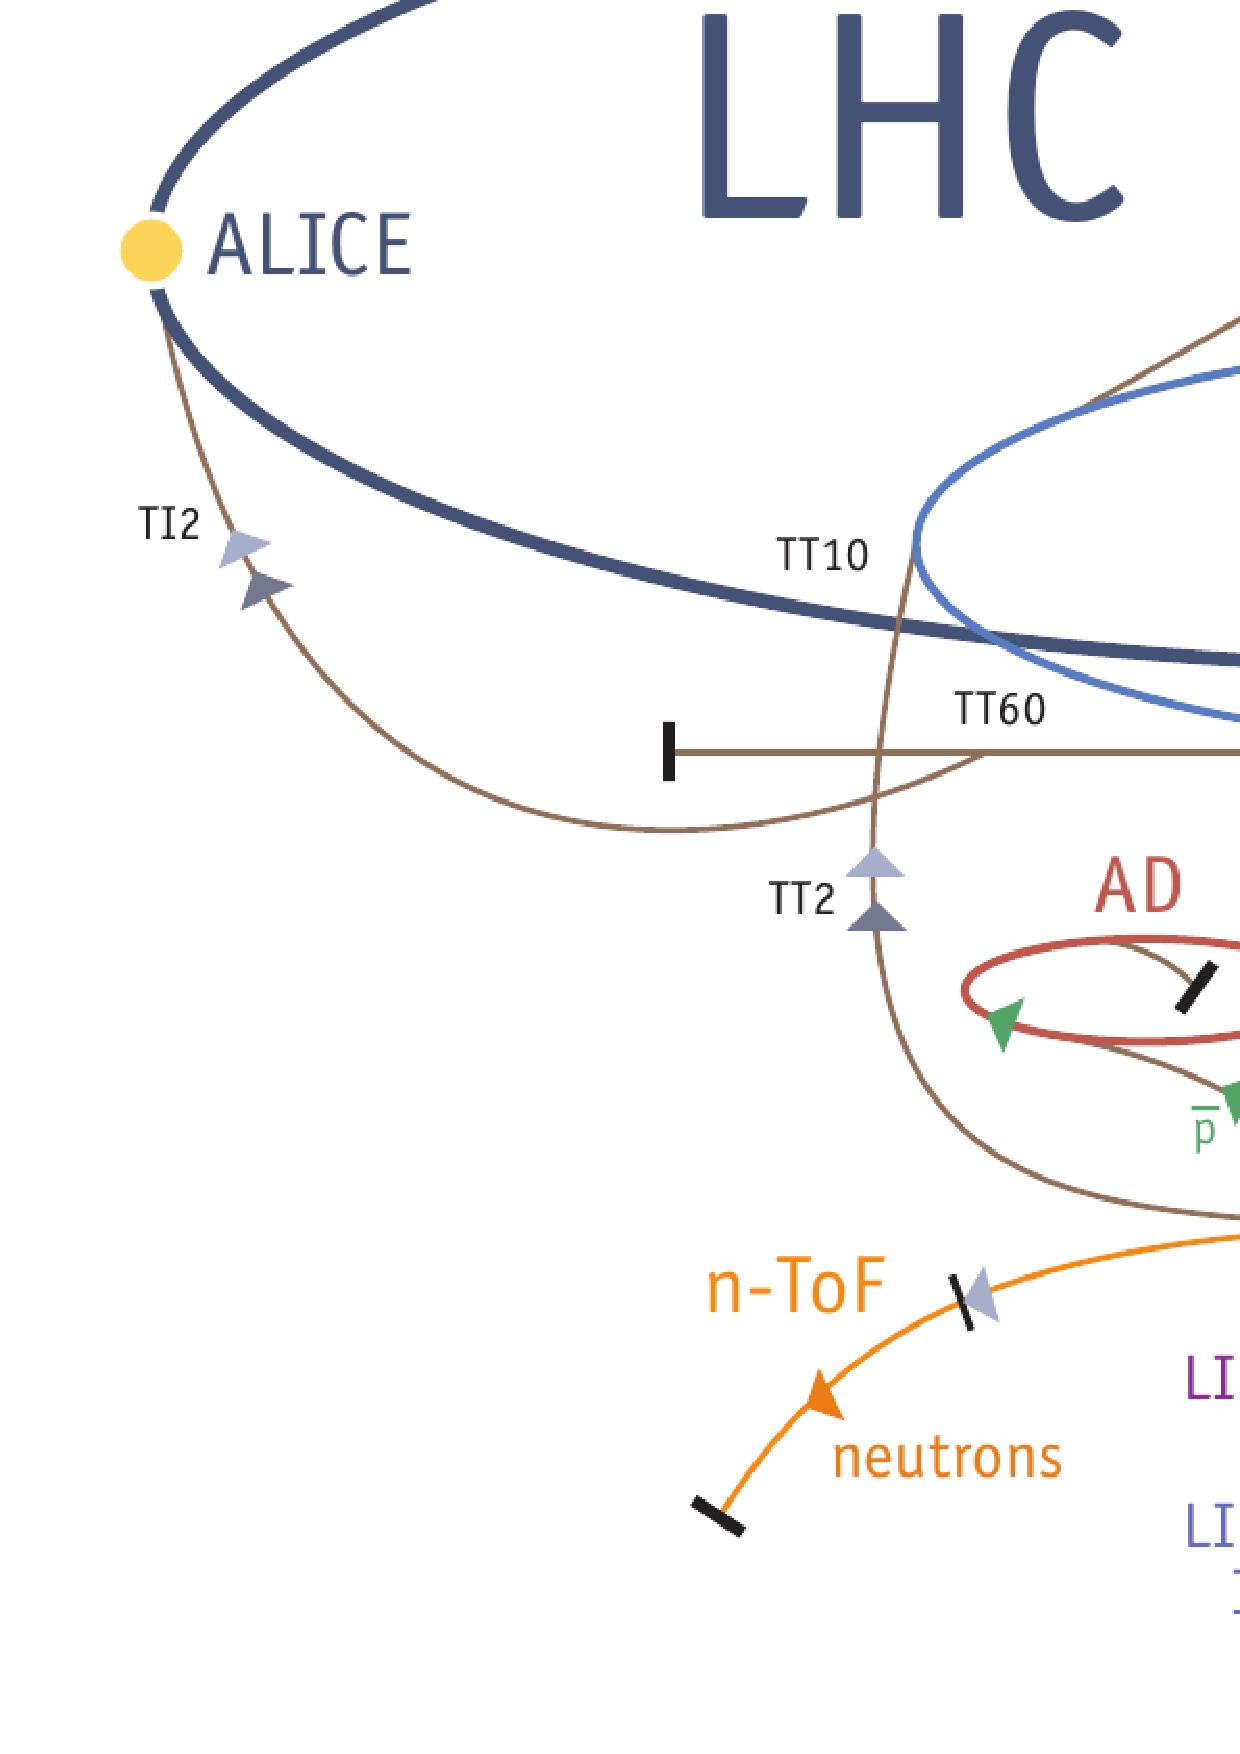
\includegraphics[width=0.9\textwidth]{figures/lhc.jpg}
  \end{tabular}
  \caption{Illustration of the CERN accelerator complex including the injector chain of the LHC ring. Taken from~\cite{CERNaccelerators}.}
  \label{fig:AccComplex}
\end{figure}
\\
\\
The main goal of the LHC is to provide proton-proton collisions to the experiments with center of mass energies up to 14\,TeV in order to explore physics processes at novel energy regimes. The expected number of events $N$ for a certain type of process is given by the product of the specific cross section $\sigma$ of that process and the integral $L = \int \mathcal{L}  \, dt$ of the instantaneous luminosity $\cal L$ over time such that
\begin{equation}
  N = \sigma \cdot L . 
  \label{eq:lumi}
\end{equation}
The luminosity is a machine parameter and can be expressed for beams with Gaussian-shaped profiles as  
\begin{equation}
  \mathcal{L} = \frac{f n_{1} n_{2}}{4 \pi \sigma_{x} \sigma{y}} \cdot F
  \label{eq:lumi}
\end{equation}
with the revolution frequency $f$, the number of particles $n_1$ and $n_2$ contained in the two colliding bunches and the transverse beam sizes $\sigma_{x}$ ($\sigma_{y}$) in the horizontal (vertical) directions. In order to take the inclination of the two beams into account, the geomatrical correction factor $F$ is introduced. The nominal peak luminosity of the LHC is $10^{34} \, \mathrm{cm}^{-2} \, \mathrm{s}^{-1}$. Since the total inelastic proton-proton cross-section at a center of mass energy of 14~TeV is close to 100\,mb as indicated in Fig.~\ref{fig:CrossSections}, the expected event rate is approximately $10^9$ events per second. This is resulting in high technical challenges for the experiments. \\
\begin{figure}[!tp]
  \centering
  \begin{tabular}{c}
    \includegraphics[width=0.60\textwidth]{figures/crosssections2012_v5-1.pdf}
  \end{tabular}
  \caption{Summary of cross sections for various standard model processes in proton-proton and proton-antiproton collisions as function of the centre of mass energy. The right axis displays the correponding event rate at a luminosity of $\mathrm{10^{33}\,cm^{-2} s^{-1}}$. Taken from~\cite{bib:stirling:pcom}.}
  \label{fig:CrossSections}
\end{figure}
\\
The four main experiments are located at the four locations along the LHC ring where the beams cross in order to measure the delivered particle collisions. The two high luminosity experiments ATLAS~\cite{det::ATLAS} and CMS~\cite{Chatrchyan:2008zzk, bib:cmsptdr1} are designed for multiple purposes like precision measurements of SM quantities, search for the standard model Higgs Boson or searches for signals indicating new physics processes. The LHCb detector~\cite{det::LHCb} however is a specialised experiment focusing on the measurement of CP violation in the interactions of hadrons containing b-quarks. The only experiment designed especially for the analysis of heavy ion collisions is the ALICE~\cite{det::ALICE} detector with the main emphasis on the physics of strongly interacting matter at extreme energy densities like for instance quark-gluon plasma.

\section{The CMS Experiment}
\label{sec:cms}
The CMS detector is one of the two experiments at the LHC designed to address a multitude of physics questions. In addition to tests of the SM at the TeV scale, studies of the nature of elektroweak symmetry breaking which might show up in the presence of a Higgs boson and searches for so far unknown particles pointing to e.g. new symmetries in nature are the primary targets of these experiments. These ambitious physics goals can only be achieved by fully exploiting the by now unprecedented collision energy and luminosity.\\
\\
The CMS detector with its typical cylindrical design of different sub-detector components around the beam line is designed to perfectly meet these particular conditions. A sketch of the CMS detector and the different sub-detectors is shown in Fig.~\ref{fig:CMS}.
\begin{figure}[!tp]
  \centering
  \begin{tabular}{c}
    \includegraphics[width=1.0\textwidth]{figures/Figures_Experimental_Apparatus_CMS_perspective.png}
  \end{tabular}
  \caption{A perspective view of the CMS detector~\cite{Chatrchyan:2008zzk}.}
  \label{fig:CMS}
\end{figure}
As a typical high-energy particle experiment the CMS detector makes mainly use of tracking detectors and calorimeters to measure particles' momenta, energy depositions and flight directions in order to identify the objects emerging from the particle collisions. The entire CMS detector with a length of 21.6\,m and a diameter of 14.6\,m results in a total weight of 12500\,t. \\  
The following sections comprise a description of the CMS detector and individual sub-detector components focusing on the detector parts most relevant for the analyses presented in this thesis. A detailed discussion of the detector design can be found in~\cite{Chatrchyan:2008zzk, bib:cmsptdr1}.

\subsection{Coordinate Conventions and Kinematic Variables}
\label{subsec:cms_coordinates}
In order to describe the particle collisions, the CMS experiment makes use of a right-handed coordinate system with its origin at the center of the detector at the nominal interaction point. While the z-axis is defined along the direction of the beam, the x-axis points to the center of the LHC ring and the y-axis vertically upwards. In this xy-plane the azimuthal angle $\phi$ is measured where $\phi = 0$ coincides with the x-axis. The polar angle $\theta$ however is defined with respect to the z-axis. A quantity closely related to the polar angle is the pseudorapidity $\eta$ defined as
\begin{equation}
\eta = \mathrm{-ln} \left[\mathrm{tan} \left(\frac{\theta}{2} \right)\right]
\end{equation}
which is widely used in experimental particle physics as rapidity differences are Lorentz invariant. A pseudorapidity $\eta = 0$ corresponds to the direction perpendicular to the beam while $|\eta| \rightarrow \infty$ points along the beam. Based on the pseudorapidity the Lorentz invariant distance between two objects $\Delta$R can be written as
\begin{equation}
\Delta \mathrm{R} = \sqrt{(\Delta \eta)^2 + (\Delta \phi)^2} \, .
\end{equation}
At the LHC the initial conditions of the primary collisions are not known as the specific energy fraction of the proton which each parton carries can not be identified. Thus conservation of the total momentum can not be utilized directly to describe the momentum balance in the final state. However, it is known that the initial particles have no significant momentum orthogonal to the beam axis which is referred to as transverse momentum 
\begin{equation}
\pt = p \cdot \mathrm{sin}\theta \, .
\end{equation}
Thus, momentum conservation in the transverse plane is used to describe the final state conditions. Any difference between the total sum of all transverse momenta and zero is considered as missing energy \met and often exploited to describe undetected particles.

\subsection{Superconducting Magnet}
\label{subsec:cms_magnet}
The CMS experiment makes use of a large superconducting solenoid magnet which is a crucial component of the whole detector design and provides a magnetic field of up to 4\,T. It allows to precisely determine the momenta and charge of charged particles from the bended tracks that they follow in the magnetic field.\\
With a length of 12.5\,m and a diameter of the free bore of 6.3\,m the total cold mass reaches 220\,t. It is made up of a niobium-titanium coil which is winded in 4-layers. This configuration allows a storage of 2.6\,GJ energy at full current. A 10000\,t heavy-weight iron yoke is responsible for the return of the magnetic flux.

\subsection{Inner Tracking System}
\label{subsec:cms_tracker}
The tracking system of the CMS experiment is the innermost part of the detector and installed directly around the interaction point completely contained in the bore of the magnet system. Its' purpose is to precisely measure the trajectories of charged particles arising from the collisions as well as to reconstruct secondary vertices. Due to the location close to the interaction point the tracking system has to cope with a high particle flux crossing the tracker associated with each bunch crossing. Hence high requirements on response time and granularity are set in order to properly identify the particles' tracks. \\
In order to fulfill these tasks the CMS experiment makes use of a tracker design based on silicon detectors. It consists of mainly two components: the innermost part is made of silicon pixel detectors while these are surrounded by silicon strip modules. In total they add up to an active area of 200\,$\mathrm{m}^2$ with a length of 5.8\,m and a diameter of 2.5\,m covering the detector up to $|\eta| = 2.5$. A schematic overview of the whole tracking system is shown in Fig.~\ref{fig:CMS_tracker}. 
\begin{figure}[!tp]
  \centering
  \begin{tabular}{c}
    \includegraphics[width=0.9\textwidth]{figures/Figures_Experimental_Apparatus_Tracker.png}
  \end{tabular}
  \caption{Sketch of the CMS tracking system in a $rz$-view. Each tracker module is represented by one line. Taken from~\cite{Chatrchyan:2008zzk}.}
  \label{fig:CMS_tracker}
\end{figure}
\begin{description}
 \item \textbf{Pixel Detector:} The pixel detector consists of three barrel layers which extend from 4.4\,cm to 10.2\,cm and two endcap disks on each side. In total there are 1440 pixel modules installed. The size of one pixel cell is 100 x 150 $\mu m^2$ providing similar track resolution quality in $r-\phi$ and $z$ direction. This configuration provides for almost the whole range up to $|\eta| = 2.5$ three precise tracking hits. This is especially important for the reconstruction of secondary vertices.
 \item \textbf{Silicon Strip Tracker:} The silicon strip detector which extends to a radius of 1.1\,m comprises the pixel tracker. The more than 15000 individual strip detector modules are arranged in an inner and an outer detector part. The inner part of the strip tracker is build by the four Tracker Inner Barrel (TIB) layers which are accompanied by the three Tracker Inner Disks (TID) at the end sides. This inner part provides up to four track measurements in the $r-\phi$ plane. The TIB/TID system lies within the Tracker Outer Barrel (TOB) consisting of another six barrel layers while it is complemented by the Tracker EndCaps (TEC) which add another nine disks at each side of the tracking system. This layout provides at least around nine hits within the silicon strip system. 
\end{description}
The tracking system with the desgin described above provides a very good impact parameter resolution and tracking efficiency~\cite{bib:cmstdr:tracker}. The impact parameter resolution is of the order of $<$ 35\,$\mu$m in the plane perpendicular to the beam (for particles with \pt $>$ 10\,GeV) and reaches 75\,$\mu$m in the longitudinal direction. Also the track reconstruction efficiency is expected to show a very good performance. The track reconstruction efficiency of high energetic electrons is above 90\%, that of charged hadrons up to 95\% (for \pt $>$ 10\,GeV) and that for muons even better than 98\% in the whole covered region up to $|\eta| = 2.5$ already for muons with very low transverse momenta around 1\,GeV. Altogether, the relative transverse momentum resolution reaches a level of 1-2\% for high momentum tracks ($\approx$ 100\,GeV) in the central barrel for $|\eta| < 1.6$.
 

\subsection{Electromagnetic Calorimeter}
\label{subsec:cms_ecal}
The CMS experiment makes use of a homogeneous electromagnetic calorimeter (ECAL) in order to precisely measure the energy deposits of electrons and photons. It is installed around the inner tracking system covering a range up to $|\eta| = 3.0$ and consists of lead tungstate (PbW$\mathrm{O}_4$) crystals. These have been chosen as they provide a high density, short radiation length and a small Moli\`{e}re radius and hence allow to build a compact calorimeter with a fine granularity. As 80\% of the scintillation light is emitted within 25\,ns, this matches well the bunch crossing rate of the LHC machine. In order to collect the radiated light photodiodes are glued to the back of each crystal. \\
An overview of the ECAL layout is shown in Fig.~\ref{fig:CMS_ecal}. The individual sub-components are the following:
\begin{figure}[!tp]
  \centering
  \begin{tabular}{c}
    \includegraphics[width=0.9\textwidth]{figures/Figures_Experimental_Apparatus_ECALRapidity.png}
  \end{tabular}
  \caption{View of one quarter section of the CMS electromagnetic calorimeter in a yz-view. Taken from~\cite{bib:cmsptdr1}.}
  \label{fig:CMS_ecal}
\end{figure}
\begin{description}
 \item \textbf{Barrel ECAL (EB):} The barrel detector of the ECAL covers the pseudorapidity region up to $|\eta| = 1.479$. Within a radius of about 1.3\,m a total number of 61200 crystals are installed. Each of them has a length of 230\,mm resulting in a radiation length of 25.8 $\mathrm{X_0}$. The crystal cross-section in $(\eta, \phi)$ is $(0.0174, 0.0174)$. Avalanche photodiodes are used to detect the emitted scintillation light.
 \item \textbf{Endcap ECAL (EE):} The EB is complemented on each side by an endcap which consists of two d-shaped halfs. The ECAL endcaps extend from $|\eta| = 1.479$ to $|\eta| = 3.0$. In total they contain another 14648 crystals with an individual length of 220\,mm corresponding to 24.7 $\mathrm{X}_0$. For the collection of scintillation light vacuum phototriodes are used in the endcaps.
 \item \textbf{Preshower (ES):} In front of the endcap crystals a preshower detector is placed. It covers the pseudorapidity range of $|\eta| = 1.653 - 2.6$. The main purpose is to identify photons emerging from the decay of neutral pions. It is a two-layer sampling calorimeter with lead as absorber material and silicon strip sensors measuring the deposited energy. The total thickness of the preshower is 20\,cm (3 $\mathrm{X_0}$).
\end{description}
In order to achieve a stable and uniform energy measurement across the whole ECAL an accurate calibration is of crucial importance. In addition to the calibration of the absolute energy scale especially channel-to-channel effects -- referred to as intercalibration -- have to be accounted for which is mainly done based on physics events. Changes in the transparency of the ECAL crystals during operation caused by irradiation are monitored by a dedicated laser system based on the injection of reference laser pulses into the crystals. The typical achievable relative energy resolution for 120 GeV electrons with this calorimeter configuration is of the order of 0.5\%.

\subsection{Hadron Calorimeter}
\label{subsec:cms_hcal}
In addition to the previously described electromagnetic calorimeter, the calorimetry of the CMS experiment is completed by the hadron calorimeter (HCAL). It is designed to provide an accurate energy measurement of hadron jets and indirectly also of invisible particles like e.g. neutrinos by the determination of missing transverse energy. In order to obtain a measure of the missing transverse energy it is important that the calorimeter is hermetic in the sense that it provides a large geometric coverage to potentially measure all particles emerging from an interaction. Thus the HCAL is build such that a pseudorapidity range up to $|\eta| = 5.2$ is comprised. \\ 
The hadron calorimeter completely surrounds the inner tracking system and the electromagnetic barrel calorimeter while it is mainly contained within the magnet system. Hence its radial dimensions are limited on the one hand by the outer circumference of the barrel ECAL and on the other hand by the inner border of the magnet coil. To ensure that the complete hadronic showers are contained in the HCAL, an additional calorimeter component is installed outside the solenoid in the barrel part. \\
An overview of the layout of the CMS hadron calorimeter is shown in Fig.~\ref{fig:CMS_hcal}. It is a typical sampling calorimeter with alternating layers of absorber material and active scintillator layers. The individual sub-components are the following:
\begin{figure}[!tp]
  \centering
  \begin{tabular}{c}
    \includegraphics[width=0.9\textwidth]{figures/Figures_Experimental_Apparatus_HCAL.png}
  \end{tabular}
  \caption{Longitudinal view of one quarter of the CMS detector showing the location of the individual HCAL sub-detector parts. Taken from~\cite{Chatrchyan:2008zzk}.}
  \label{fig:CMS_hcal}
\end{figure}
\begin{description}
 \item \textbf{Hadron barrel (HB):} The barrel part of the CMS hadron calorimeter covers the pseudorapidity range up to $|\eta| = 1.3$ and is composed of two half barrels each containing 36 identical azimuthal wegdes. These wedges hold the absorber plates which are flat brass plates arranged parallel to the axis of the beam. For reasons of stability the first and last layers are made of stainless steel. The total thickness of the absorber material ranges from 5.82 interactions lengths ($\lambda_I$) at $|\eta| = 0.0$ to 10.6\,$\lambda_I$ at $|\eta| = 1.3$. The 17 active plastic scintillator layers alternate with the absorber plates and have a segmentation in $(\Delta \eta, \Delta \phi)$ of (0.087, 0.087).\\
Each half barrel is divided into 16 $\eta$-regions for which the individual tiles are optically linked together using wavelength shiftig fibres and thus form so-called \textit{HCAL towers}. The read-out of each longitudinal tower is carried out using pixelated hybrid photodiodes.
 \item \textbf{Hadron outer (HO):} The calorimeters in the central pseudorapidity region do not provide a sufficient depth in order to fully contain all hadronic showers. Therefore the HB is complemented by the outer hadron barrel part which is placed outside the solenoid covering $|\eta| \le 1.26$. The HO makes use of the solenoid as additional absorber material and adds another one or even two layers in the most central part of scintillators to the barrel region. Thus the total depth is extended to 11.8\,$\lambda_I$.
 \item \textbf{Hadron endcap (HE):} The hadron barrel calorimeter is supplemented by the hadron endcap. It is mounted on the endcap iron yoke and covers the pseudorapidity region of $1.3 \le |\eta| \le 3.0$ using 18 scintillator layers inserted into brass absorber plates. The granularity of the endcap calorimeter is the same as for the barrel up to $|\eta| = 1.6$ and gets coarser for larger pseudorapidities with $(\Delta \eta, \Delta \phi) \approx (0.17, 0.17)$.
 \item \textbf{Hadron forward (HF):} The forward hadron calorimeter extends the pseudorapidity coverage from $|\eta| = 2.9$ (slightly overlapping with the HE) up to $|\eta| = 5.2$. It is located 11.2\,m from the nominal interaction point and has to be in particular radiation hard to cope with the vast particle flux. Thus the HF is made of steel absorber plates with radiation hard quartz fibres integrated as active material. These fibres are arranged parallel to the beam line and form towers with a size in $(\Delta \eta, \Delta \phi)$ of $\approx$ (0.175, 0.175). The signal is detected as Cerenkov light originating from the quartz fibres.
\end{description}
Similar to the ECAL also the performance of the HCAL has to be well calibrated and further monitored during operation. Thus an initial calibration using a radioactive source is combined with test beam data to derive the absolute energy scale. A continous update of this calibrations is performed using isolated energetic particles e.g. from decays of W or Z bosons. 

\subsection{Muon System}
\label{subsec:cms_muon}
The outermost part of the CMS detector -- as seen from the interaction point -- is made up of the muon system. This important component of the detector is assembled in the return yoke of the CMS magnet and consists of a central barrel cylinder which is complemented by endcap disks in the forward region. This results in a coverage of the pseudorapidity range up to $|\eta| = 2.4$. In the barrel part four layers of detectors are installed alternating with the iron yoke while the detectors in the endcap are mounted on four discs perpendicular to the beam. In total about 25000\,$\mathrm{m}^2$ detection planes are employed. The layout of the muon system is illustrated in Fig.~\ref{fig:CMS_muon}. \\
In order to feature a good muon momentum resolution given the different radiation conditions and variations in the homogenity of the magnetic field depending on the pseudorapidity region it is made use of three different types of gaseous detectors. These different types of tracking chambers are described in the following:
\begin{figure}[!tp]
  \centering
  \begin{tabular}{c}
    \includegraphics[width=0.9\textwidth]{figures/Figures_Experimental_Apparatus_MuonDetector.png}
  \end{tabular}
  \caption{Taken from~\cite{bib:cmsptdr1}.}
  \label{fig:CMS_muon}
\end{figure}

\begin{description}
 \item \textbf{Drift tube (DT) chambers:} In the barrel region for $|\eta| < 1.2$ where the background due to neutrons is low and residual effects from the magnetic field likewise the muon system is equipped with drift tube chambers. While in all four stations in the barrel the muon coordinates in the $r\phi$-plane are measured, only the first three layers provide also a measurement of the $z$-direction. The maximum drift length was chosen to be 21\,mm resulting in a negligible occupancy while keeping the number of active channels at an acceptable level. Furthermore, a technology based on tubes was chosen avoiding the issue of possibly broken wires. The resolution in $r\phi$ is designed to reach a precision of 100\,$\mu$m.
 \item \textbf{Cathode strip chambers (CSC):} The endcap regions are equipped with cathode strip chambers and cover the pseudorapidity range $0.9 < |\eta| < 2.4$. These are chosen as they provide a fast response time and fine segmentation while they are resistant against radiation. Thus they are well suited for the forward region where the muon and background rates are largely increased and the magnetic field is high and non-uniform. The CSCs which are multiwire proportional chambers where anode wires are interlaced with cathode panels perform a precise position measurement in the $r\phi$ bending plane with a spatial resolution of 75-150\,$\mu$m. 
 \item \textbf{Resistive plate chambers (RPC):} Resistive plate chambers are used to complement the drift tube and cathode strip chambers in the range $|\eta| < 1.6$. These are gaseous parallel-plate detectors with a spacial resolution coarser than the DTs and CSCs but usable at high particle rates while providing a very fast response and good time resolution. Thus they are able to very efficiently detect the correct bunch-crossing a muon track is associated to. 
\end{description}
The global muon reconstruction efficiency is in general about $95-99\%$ and only drops for some $|\eta|$ regions like e.g. in the transition region between the barrel and endcap part around $|\eta|=1.2$. Since muons reaching the muon system are affected by multiple scattering the resolution for muons with low transverse momenta below $\approx$ 200\,GeV is in general better based on the inner tracking system than for the muon system alone. For highly energetic muons it is comparable. In general, the muon momentum resolution can be improved by combining the information from the inner tracker and the muon system due to an improved fault finding. This combined approach results in a relative muon momentum resolution for muons with high momenta around 1\,TeV of about 5\%.

\subsection{Trigger System}
\label{subsec:cms_trigger}
The LHC operating at design conditions provides particle collisions with an interaction rate of 40\,MHz. This results in an enormous amount of data events which have to be processed and stored for later offline analyses. With an approximate event size of 1 MB it is technically impossible to record all such events. However, as illustrated in Fig.~\ref{fig:CrossSections} the event rate of interesting potentially new physics events is orders of magnitudes smaller than the proton-proton cross section. Thus, this allows to already perform online a suitable event preselection in order to reduce the amount of data to a storable size still containing the information of interest. Hence, the trigger system also makes up the first step in the physics analysis process.\\
In order to achieve the necessary rate reduction, the CMS experiment makes use of a two-stage trigger system. This is described in the following.
\begin{description}
\item \textbf{Level-1 (L1) Trigger:} The L1 Trigger consists of custom-made fast programmable hardware. It makes use of data received from fast detector components -- namely the calorimeters and the muon system -- at reduced granularity. For instance at L1 the calorimeter is divided into so-called \textit{trigger towers} which cover an area in $(\eta, \phi)$ of $(0.087, 0.087)$ up to $|\eta| = 1.74$ and get even coarser for higher $|\eta|$. At L1 the trigger decision is based on energy deposits in those trigger towers or certain hit patterns in the muon chambers forming trigger primitive objects as electrons/photons, muons or jets and global quantities like sums of \et or \met. Events are accepted, if these trigger objects pass some predefined criteria like certain \pt thresholds. The L1 trigger latency between the actual bunch crossing and the delivery of the L1 trigger decision to the front-end electronics is 3.2\,$\mu s$. During this period the high resolution data is pipelined in readout buffers for further processing. Following this procedure the L1 trigger reduces the event rate to 100\,kHz.
\item \textbf{High-Level Trigger (HLT):} Events that are accepted by the L1 are transferred to the High-Level trigger for further processing. The HLT is a software system running on several thousand commercial processors. It has access to the full information from all sub-detectors and performs an event reconstruction similar to the later offline reconstruction. Thus it allows a further rate reduction to the final output rate of a few hundred Hz of events that are finally stored for analyses. Since the HLT is software based, it allows to continously adjust the used algorithms in order to perfectly meet changing conditions during operation.
\end{description}

\section{LHC Operation and Data Taking}
\label{sec:data}
\begin{figure}[!tp]
  \centering
  \begin{tabular}{c}
    \includegraphics[width=0.7\textwidth]{figures/int_lumi_cumulative_pp_2.pdf}
  \end{tabular}
  \caption{Cumulative integrated luminosity versus day delivered to CMS during stable beams for pp collisions. Different data-taking periods are indicated as follows: green for 2010, red for 2011 and blue for 2012. Taken from~\cite{bib:lhc:lumi12}.}
  \label{fig:lhc_data}
\end{figure}
The LHC was put into operation the first time in September 2008. After a major cooling incident only a few days later requiring a longer technical stop, beams were circulated again in November 2009. The first collisions at a center of mass energy of 7\tev finally took place end of March 2010~\cite{bib:lhcmachineoutreach}. In the following running period in 2010, data corresponding to an integrated luminosity of 44.2\pbinv were delivered to the experiments with a maximum peak instantaneous luminosity of $2.05 \times 10^{32} \cm^{-2} \second^{-1}$. These data allowed intense studies of the detector performance and made first searches for new physics possible. The next data taking period performed during 2011 at the same center of mass energy even lead to much more pp collision data provided to the experiments with a total amount of 6.1\fbinv reaching a peak instantaneous luminosity of $3.5 \times 10^{33} \cm^{-2} \second^{-1}$. Following another technical shutdown during winter, the center of mass energy was finally increased to 8\tev for the running period during 2012 and the peak luminosity reached with values of up to $7.7 \times 10^{33} \cm^{-2} \second^{-1}$ already almost design conditions. In total, 23.3\fbinv of integrated luminosity pp collisions were produced by the LHC operating at stable beam conditions. The evolution of the integrated luminosity versus days is also illustrated in Fig.~\ref{fig:lhc_data}. \\
\begin{figure}[!tp]
  \centering
  \begin{tabular}{c}
    \includegraphics[width=0.7\textwidth]{figures/pileup_pp_2012.pdf} 
  \end{tabular}
  \caption{Mean number of interactions per bunch crossing in pp collisions at $\sqrt{s} = 8$\tev. Taken from~\cite{bib:lhc:lumi12}.}
  \label{fig:lhc_pileup}
\end{figure}
During most of the operation in 2012, the LHC was circulating 1380 bunches per beam with a distance of 50\,ns. The average bunch intensity, \ie the number of protons per bunch, was varying from $1.6$ to $1.7 \times 10^{11}$ extending already the design value~\cite{bib:lhc:lumi12, Lamont:2013cma}. This was on average resulting in 21 pp collisions per bunch crossing. This process of multiple interactions per bunch crossing is known as \textit{pileup}. An overview of the pileup profile observed in collision data taken in 2012 is given in Fig.~\ref{fig:lhc_pileup}. The maximum number of pileup events even reached a value of $\approx 40$. This effect caused by the required high luminosity generates challenging conditions for the experiments as many objects arising from such multiple interactions have to be asigned to the correct process and particular collision objects have to be filtered. Dedicated techniques in order to cope with this problem have been developed of which some are discussed in Chapter~\ref{chap:Objects}.

\section{Event Simulation}
\label{sec:simulation}
An important tool in high energy physics is the use of simulation in order to acquire a good understanding of the behaviour of particle collisions and related collision products observed in the detector. Thus, simulated events often serve as benchmark for the development of new detector concepts. Moreover, they are heavily exploited in the validation and interpretation of the results of actual collision experiments, likewise for the LHC. For instance simulated events are used to derive expectations for certain physics properties or the detector performance. In particular they allow to estimate how signals of new physics events would look like in the experiment. \\
This section provides a brief introduction to the principles of event simulation in hadron collisions and introduces some event generators including different approaches for the simulation of the detector. A broader overview of event simulation and respective generators for LHC physics can be e.g. found in~\cite{Seymour:2013ega, Buckley:2011ms}. \\
\\
The simulation of high energy collisions is a quite challenging task as each collision involves typically several hundreds of particles with momenta ranging over some orders of magnitude. Furthermore, the collisions being subject to quantum chromodynamics are only calculable within approximation schemes where also numerical methods do not provide solutions within a reasonable amount of time. Thus, event simulation is primarily utilizing \textit{Monte Carlo} (MC) techniques which rely on the repeated sampling of random numbers, \cf e.g.~\cite{bib:MCMethod}. For convenience events obtained from simulation are often denoted by the label 'MC' in this thesis. \\
Typically, the generation of an event follows several subsequent steps which are illustrated in Fig.~\ref{fig:mc_gen} and described in the following: 
\begin{figure}[!tp]
  \centering
  \begin{tabular}{c}
    \includegraphics[width=0.9\textwidth]{figures/MCGeneration.pdf} 
  \end{tabular}
  \caption{Sketch of individual steps in the generation process of simulated events.}
  \label{fig:mc_gen}
\end{figure}
\begin{description} 
 \item \textbf{Hard process:} The first step in the simulation of collision events is the description of the nominal proton-proton interaction which is typically referred to as \textit{hard process}. The proton itself is not a fundamental particle but exhibits an internal structure \todo{Quelle: Proton Struktur}. The constituents of which a proton is made off are known as \textit{partons}. Thus two protons interact when there is a momentum transfer \textit{Q} taking place between two individual partons. The probability for individual partons to take part in the hard interaction is parametrized by the \textit{parton-distribution functions} (PDFs) which have been determined experimentally \todo{Quelle:PDFs}. The value of $x$ denotes the fraction of the longitudinal momentum carried by an individual parton. Consequently, the initial state of a proton-proton collision is not exactly known. Nevertheless, the cross section of a specific process can be calculated following the \textit{factorization theorem}~\cite{Collins:1987pm, Collins:1989gx}. Here, the hard interaction is described via perturbation theory and low-energy processes are considered in the phenomenological models of the respective PDFs. Thus the cross section for a process $ab \rightarrow n$ is given according to
\begin{equation}
 \sigma = \sum_{a,b} \int_{0}^{1} dx_{a} \, dx_{b} \int f_{a}(x_{a}, \mu_{F}) f_{b}(x_{b}, \mu_{F}) \, d\hat{\sigma}_{ab \rightarrow n} (\mu_{F}, \mu_{R}). 
\end{equation}
Here, $f(x, \mu_{F})$ are the PDFs of the interacting protons which depend on the factorization scale $\mu_{F}$ whereas $\sigma_{ab \rightarrow n}$ indicates the parton-level cross section for the production of a final state $n$ from partons $a$ and $b$. This parton-level cross section depends on the final-state phase space, the factorization scale and the renormalisation scale $\mu_{R}$ as well as the corresponding matrix element. The factorization and renormalization scale are unphysical and have to be chosen for the generation process. Often the process possesses a typical hard scale $Q^{2}$ so that the choice $\mu_{F} = \mu_{R} = Q^{2}$ is made. However, this choice is not fixed by first principles.
\item \textbf{Parton shower:} After the production in the hard interaction the outgoing partons start to form a shower, \ie cascades of further partons emerge. Typically, this happens with descending amounts of momentum transfer from the high scales down to low scales around 1\gev. This evolution is typically described by a probabilistic shower algorithm. In addition to a parton shower related to the outgoing partons which is referred to as \textit{final-state radiation} (FSR), partons can already radiate off other partons before the actual hard process takes place. This effect is known as \textit{initial-state radiation} and can be described by similar principles as FSR. However, in the case of ISR it is inevitable to consider that not all partons from the ISR shower necessarily take part in any hard process and thus have to be related to the proton remnant.  
 \item \textbf{Hadronization:} \textit{fragmentation functions}
 \item \textbf{Decay:}
 \item \textbf{Underlying event:}
\end{description}
These processes are the basis of various event generators which differ in some aspects concerning the treatment of individual sub-processes in the event simulation. Some of such generators, which are used in this thesis, are the following:  
\begin{description}
 \item \textbf{\pythia:}
 \item \textbf{\madgraph:}
 \item \textbf{\herwig:}
\end{description}
In order to evaluate the interaction of the generated particles with the detector material the passage of the particles through the detector is simulated with a model of the CMS apparatus. Depending on the details of the detector model this is referred to as \textit{full simulation} or \textit{fast simulation} \todo{Quellen}. Some of the differences are described in the following: 
\begin{description}
 \item \textbf{Full simulation:} 
 \item \textbf{Fast simulation:} 
\end{description}
Finally, recorded collision data as well as simulated events are present in the same data format. This allows to use the same reconstruction techniques in order to build the event and derive physics objects from the obtained detector signals.




\chapter{Object Reconstruction and Particle Identification} \label{chap:Objects}
Particles produced in the pp collisions traverse through the detector and interact with the detector sub-components in a characteristic manner. Thus, it is possible to reconstruct the corresponding event and identify the types of particles which actually emerged from the collision. \\
The approach for the event reconstruction and identification of specific particles used in CMS is discussed in this Chapter. First, the \textit{Particle-Flow (PF) algorithm} used for a global description of the collision event is introduced. Beyond that, in particular the reconstruction of jets is discussed in Section~\ref{sec:jets_reco}. Furthermore, the identification of decays from b-hadrons and boosted top quarks is reviewed in Sections~\ref{sec:btagging} and~\ref{sec:boosted_tops}, respectively.
\section{Global Event Description with the Particle-Flow Algorithm at CMS}
\label{sec:pf_algo}
The CMS experiment introduced the Particle-Flow algorithm for the reconstruction of collision events. This algorithm is designed to identify all stable particles in an event and can be applied to data events as well as to simulated events in an identical manner. Electrons and photons, charged and neutral hadrons as well as muons are thereby distinguishable and all sub-components of the detector are used by the PF algorithm to reconstruct the particles four-momenta. The CMS detector is very well suited for this task. The silicon tracker enclosed by the uniform magnetic field enables a very efficient track reconstruction yielding only a small track fake rate down to small transverse momenta of $150$\,MeV/c. Furthermore, the strength of the magnetic field together with a high ECAL granularity allows photons to be separated from charged-particle energy deposits. A detailed introduction to the PF algorithm can be found in~\cite{CMS-PAS-PFT-09-001}. \\ 
The event reconstruction starts with the identification of fundamental objects in the sub-detectors which are charged-particle tracks, calorimeter clusters and muon tracks. Tracks emerging from charged particles are formed following an iterative tracking algorithm~\cite{Adam:934067}. Starting from an initial seed trajectory, tracks are extrapolated to further tracker layers by taking into account multiple scattering and energy loss in the material following the equations of motion of a charged particle in a constant magnetic field. Each step proceeds with a removal of unambiguously allocated hits from the previous iteration. With this approach a high tracking efficiency as well as a low fake track rate can be achieved which is a crucial requirement for a successful particle-flow event reconstruction. Furthermore, calorimeter clusters are formed in each sub-detector separately based on adjacent calorimeter cells. Neighbouring cells are combined to form clusters when their energy exceeds a pre-defined threshold. \\
A particle traversing through the detector gives typically rise to several of such elementary components so that a dedicated link algorithm is applied in order to connect these elements and form blocks while removing a potential double-counting of the same object in different detector parts. First, charged-tracks are associated to calorimeter clusters, if the extrapolated trajectory matches the cluster within the cluster boundaries. This is done considering effects like gaps and cracks between detector components, uncertainty on the shower position or multiple-scattering. Photons from Bremsstrahlung are considered by extrapolating also tangents of the tracks to the respective energy clusters. In a similar manner ECAL and HCAL clusters can be connected to each other as well by linking clusters in the more granular calorimeter to clusters in the less granular one. At last global muons can be defined by associating charged-tracks from the tracker with muon tracks reconstructed in the muon system. \\
After the identification of such blocks of elements the PF algorithm proceeds to finally create a list of all particles contained in the event applying dedicated quality criteria interpreting the blocks in terms of particles. The identification of muons and a removal of their tracks from the blocks is followed by an assignment of electrons and associated Bremsstrahlung from tracks and linked ECAL clusters. After these have been removed from the list of blocks as well, remaining good quality tracks are considered to be charged hadrons. Their momenta are determined from combining the track momentum and the respective energy in the calorimeter cluster. If the cluster energy largely exceeds the measured momentum from the track beyond the detector resolution, it constitutes a photon and if the excess is larger than the total ECAL energy also a neutral hadron. Finally, remaining ECAL and HCAL clusters not linked to any track give rise to photons and neutral hadrons. \\
The complete set of particles can then be used to derive further objects and quantities like e.g. jets as discussed in Section~\ref{sec:jets_reco}, missing transverse energy $E_{T}^{\mathrm{miss}}$ which is the magnitude of the vector momentum imbalance perpendicular to the beam direction or decay products of tau leptons. More detailled information on the specific quality criteria required for the identification of certain particles is given in the Chapters~\ref{chap:Resolution},~\ref{chap:RA2} and~\ref{chap:Stop} for each analysis presented in this thesis, individually.

\section{Reconstruction of Jets}
\label{sec:jets_reco}
As stated already earlier jets are the experimental signatures of quarks and gluons and constitute of a collimated spray of hadrons. However, in order to identify a particular jet and relate its properties to the original parton a proper jet definition is needed. Typically, a \textit{jet algorithm} determines how to cluster particles into a jet. Furthermore, it has to be defined how to assign a momentum to the jet. At CMS, the standard procedure is to assign the four-momentum sum of all jet constituents to the jet. \\
Different jet algorithms are introduced in Section~\ref{subsec:jets_algos} followed by a discussion of different jet types used at CMS in Section~\ref{subsec:jets_types}. Furthermore, the jet transverse-momentum response is defined in Section~\ref{subsec:jets_response} and the calibration of jet energies is reviewed in Section~\ref{subsec:jets_calib}.
\subsection{Jet Algorithms}
\label{subsec:jets_algos}
\begin{figure}[!tp]
  \centering 
  \begin{tabular}{cc}
    \includegraphics[width=0.49\textwidth]{figures/herwig-parton-level-ev-kt.png} &
    \includegraphics[width=0.49\textwidth]{figures/herwig-parton-level-ev-cam.png} \\
    \includegraphics[width=0.49\textwidth]{figures/herwig-parton-level-ev-antikt.png} &
    \includegraphics[width=0.49\textwidth]{figures/herwig-parton-level-ev-siscone.png}   
  \end{tabular}
  \caption{Sample parton-level event generated with \herwig, adding many random soft particles, that is clustered with the $\mathrm{k_T}$ -algorithm (\textit{top left}), the C/A-algorithm (\textit{top right}), the SISCone-algorithm (\textit{bottom left}) and the $anti-\mathrm{k_{T}}$-algorithm (\textit{bottom right}). Colours illustrate the active areas of the resulting hard jets. Taken from~\cite{Salam:2009jx}.}
  \label{fig:jet_algos}
\end{figure}
A jet algorithm usually provides a prescription how to combine individual particles into a single jet based on some distance criterium. Good jet algorithms though should be able to identify jets that are neither sensitive to the emission of soft particles (\textit{infrared safety}) nor to the collinear splitting of particles (\textit{collinear safety}). These features named \textit{IRC safety} are desirable as otherwise e.g. cross sections would be dependent on particular effects of hadronisation involving random collinear splittings and soft emissions making it difficult to compare the results from experiments to theroretical predictions. This effect is even enforced because detectors intrinsically provide regularisation of IRC effects to some extent due to a finite resolution. Furthermore, calculations in QCD perturbation theory rely on the cancellation of divergences related to IRC processes. Thus, if jets are sensitive to such effects cancellations are not ensured and can lead to inifinite cross sections. \\
An introduction to the most commonly used jet algorithms known as \textit{cone algorithms} and \textit{sequential recombination algorithms} is given in the following. A comprehensive overview of jet algorithms and properties can be found in~\cite{Salam:2009jx}.
\begin{description}
 \item \textbf{Cone Algorithms:} Cone algorithms were the first developed jet algorithms. They are based on the general idea that the main kinematics in an event are not changed by specific effects from hadronisation and thus a jet is defined by a set of particles within a stable cone around their centre of mass. Typically, separate angular or energy parameters are used to perform the jet finding. A very common approach is implemented in \textit{iterative cone} (IC) algorithms. Here, a seed constituent $i$ which is for instance the constituent with the highest transverse momentum defines the initial direction and momenta of all constituents $j$ within a cone defined by
\begin{equation}
 \Delta R_{i,j}^2 = (\eta_i - \eta_j)^2 + (\phi_i - \phi_j)^2 < R^2
\end{equation}
are added to the momentum of the seed. The resulting direction is used as new seed direction and the whole procedure is repeated until a stable cone is achieved. The dimensionless parameter $R$ hence defines the jet radius. After the finding of such a jet, all constituents are removed from the input list and further jets are clustered from the remaining objects. This progressive removal approach avoids to form jets with overlapping cones. However, such a procedure is not IRC safe as collinear splittings can lead to different final ensembles of jets. \\
The issue with IRC safety in cone algorithms can be avoided by instead of iteratively forming stable cones one after the other identifying all stable cone solutions at once. This procedure is denoted \textit{seedless cone} (SC) algorithm. The usage of such algorithms though is typically impractical as the computation time increases exponentially with the number of particles to be considered so that even for 100 particles it is not solveable at any reasonable timescale. A feasible implementation of a seedless cone algorithm featuring only a logarithmic time-dependence is given by the SISCone algorithm~\cite{Salam:2007xv}. As it is usually nonetheless still more time consuming than sequential algorithms as described in the next part, the SISCone algorithm is not used by CMS.
 \item \textbf{Sequential Recombination Algorithms:} The basic concept of sequential clustering algorithms is to group in an iterative procedure pairs of particles together based on some distance measure and thus reconstructs to some extent the evolution of a parton shower. A suitable metric to be used at hadron colliders where the total energy of a collision is unknown based on variables invariant under longitudinal boosts is 
\begin{equation*}
d_{ij} = \mathrm{min}(k_{T,i}^{2p}, k_{T,j}^{2p}) \frac{\Delta R_{ij}^2}{R^2}
\end{equation*}
\begin{equation*}
d_{iB} = k_{T,i}^{2p}
\end{equation*}
with the distance $d_{ij}$ between final state objects $i$ and $j$ carrying transverse momentum $k_T$ and the distance of the object to the beam $d_{iB}$. While $\Delta R_{ij}$ denotes the spatial separation in the $(\eta, \phi)$-plane, $R$ and $p$ are free parameters of the algorithm. The recombination is done by first calculating $d_{ij}$ and $d_{iB}$ for all objects in the final state by identifying the minimum value. If the minimum is $d_{ij}$, the two objects $i$ and $j$ are combined and all distances are computed again. However, if the minimum is $d_{iB}$, object $i$ is declared a jet and removed from the input list. This procedure is repeated until all objects are assigned. In this context the parameter $R$ acts as an angular cut-off and thus has a similar role as the jet radius in cone algorithms. Depending on the choice of the parameter $p$ different types of algorithms are distinguished which are all IRC safe.  \\
\todo{kT algorithm} \todo{anti-kT algorithm} \todo{C/A algorithm}
An illustration of an arbitrary example event where jets are clustered with the different jet algorithms is shown in Fig~\ref{fig:jet_algos}.
\end{description}

\subsection{Jet Types at CMS}
\label{subsec:jets_types}

\subsection{Jet Transverse-Momentum Response}
\label{subsec:jets_response}

\subsection{Jet Energy Calibration}
\label{subsec:jets_calib}

\section{Identification of b-Quark Jets}
\label{sec:btagging}
Jets arising from the hadronization of bottom quarks are usually referred to as \textit{b-jets}. As these are existent in many physics processes as e.g. the decay of top quarks, it is of essential importance to be able to identify b jets and distinguish them from jets initiated by gluons or light-flavour quarks. Typically, the identification of b-jets is denoted \textit{b-tagging} and the distinct properties of b quarks are exploited for the identification of the respective jets. In general, hadronic jets arising from the fragmentation of b quarks possess quite large masses, long lifetimes and daughter particles featuring hard momentum spectra. The CMS experiment with the ability to perform a precise charged-particle tracking and lepton identification exploits the specific b jet properties in dedicated b-tagging algorithms for an efficient b-jet identification~\cite{Chatrchyan:2012jua}:
\begin{description}
 \item \textbf{Track Counting (TC) algorithm:} A powerful discriminator for the decay products of a b hadron from prompt tracks is the \textit{impact parameter} (IP) of a track with respect to the primary vertex. Its significance can be computed by taking the ratio of the IP to its respective uncertainty. Tracks in a jet are sorted by decreasing values of the IP significance by the TC algorithm. Depending on whether the IP significance of the second or the third ranked track is chosen as discriminator value the algorithm is denoted \textit{Track Counting High Efficiency} (TCHE) or \textit{Track Counting High Purity} (TCHP) algorithm. 
 \item \textbf{Jet Probability (JP) algorithm:} The JP algorithm extends the simple TC algorithm by connecting the information about the IP from a couple of tracks in the jet. A likelihood is calculated that all tracks of the jet stem actually from the primary vertex. This appraoch can be varied by giving more weight to tracks with the highest IP significance. The maximum of such tracks is four and matches the average number of reconstructed charged particles from the decay of b hadrons. This version is called \textit{Jet B Probability} (JBP) algorithm.
 \item \textbf{Simple Secondary Vertex (SSV) algorithm:} A further useful discriminating feature for b tagging is the presence of a secondary vertex and related kinematic variables like the flight distance and direction which can be determined from the vector between the primary and secondary vertex. The SSV exploits the significance of the flight distance which is given by the flight distance divided by the associated uncertainty. Two different versions of this algorithm exist targeting on the one hand a \textit{High Efficiency} (SSVHE) and on the other hand a \textit{High Purity} (SSVHP). While the SSVHE is based on vertices with at least two associated tracks, the SSVHP uses vertices with more than three tracks. Typically, the efficiency of the algorithm is limited by the reconstruction efficiency of secondary vertices which amounts to about 65\%.  
 \item \textbf{Combined Secondary Vertex (CSV) algorithm:} The CSV algorithm provides an efficient identification of b jets also in cases when no secondary vertex could be recosntructed. It utilizes an approach combining information from secondary vertices as well as track-based lifetime information and thus is able to exceed the efficiency of SSV algorithms. Often, pseudo-vertices can be formed from tracks even when failing the reconstruction of an actual secondary vertex which allows to derive some secondary vertex related quantities. Variables used in the CSV algorithm are e.g. flight distance significance, vertex mass, number of tracks at the vertex, number of tracks in the jet or the IP sigificances for the tracks in the jet. These variables are used to compute two likelihood ratios which can be used to distinguish either c and b jets or light-parton and b jets. 
\end{description}  
Each algorithm determines a discriminator value per jet indicating how b-jet-like a jet behaves. Based on that, working points are defined corresponding to a specific minimum threshold of the discriminator value. These working points are named \textit{loose}, \textit{medium} and \textit{tight} and correspond to a misidentification probability, \ie the probability to identify a non-b jet as b jet, of $10\%$, $1\%$ and $0.1\%$ for an average jet momentum of $80$\gev, respectively. \\
\begin{figure}[!tp]
  \centering 
  \begin{tabular}{cc}
    \includegraphics[width=0.49\textwidth]{figures/figAlgo_Combined_udsgvsb_Efficienies.png} &
    \includegraphics[width=0.49\textwidth]{figures/figAlgo_Combined_cvsb_Efficienies.png} 
  \end{tabular}
  \caption{Performance curves obtained from simulation for the algorithms described in the text. (a) light-parton- and (b) c-jet misidentification probabilities as a function of the b-jet efficiency. Taken from~\cite{Chatrchyan:2012jua}.}
  \label{fig:btagging}
\end{figure}
In order to determine the quality of a particular b-tagging algorithm, typically the misidentification probability as function of the b-tag efficiency is compared for various taggers. Such a performance comparison is illustrated in Fig~\ref{fig:btagging} for the tagging algorithms described above. The misidentification probability is derived separately for light-flavour and gluon initiated jets as well as c-jets. The curves are derived from simulated multijet events using jets with $\pt > 60$\,\gev. For loose working points the b-tag efficiency is around $\approx 80-85\%$ and the JBP algorithm shows the best performance. In case of medium and tight selections, the b-tag efficiency drops to $\approx 45-55\%$ and the CSV algorithm performs best. \\
B-tagging algorithms used for analyses of data obtained at $\sqrt{s} = 8$\tev in 2012 where the TCHP, JP and CSV algorithm~\cite{CMS-PAS-BTV-13-001}. In order to compare the b-tagging performance in data and simulation two different event samples have been selected. On the one hand, an inclusive multijet sample is selected requiring at least one jet with $\pt = 60 - 500$\gev which is dominated by jets from light-flavour quarks and gluons. On the other hand, a sample dominated by top-pair production is selected requiring an electron, a muon and at least two jets with $\pt>30$\gev such that this sample is enriched in b-jets. These samples allow to compare quantities relevant for b-tagging in data and simulation like e.g. the number of secondary vertices or b-tag discriminator values. In general, quantities relevant for b-tagging show a good agreement between data and simulation with deviations within 20\%. Typically, efficiencies and misidentification probabilities are measured as function of jet transverse momentum and pseudorapidity. A potential disagreement between data and simulation can be expressed in terms of \textit{scale factors} and corrected for in analyses such that b-tagging efficiency and misidentification probability in data and simulation match. 

\section{Identification of Boosted t-Quark Jets }
\label{sec:boosted_tops}
Supersymmetric models or other scenarios describing physics beyond the Standard Model predict the extistence of new massive particles. Often, the coupling of these particles especially to quarks belonging to the third generation is sizeable like e.g. in decays of top squarks which predominantly are expected to decay into top quarks. Consequently, such processes lead to highly-energetic top-quarks in the final state which can be identified exploiting the specific properties of the top-quark. \\
\begin{figure}[!tp]
  \centering 
  \begin{tabular}{c}
    \includegraphics[width=1.0\textwidth]{figures/BoostedTops.jpg} 
  \end{tabular}
  \caption{Schematic diagrams of the decay of a top-quark in the resolved case (\textit{left}) and the boosted scenario (\textit{right}).}
  \label{fig:boosted_top}
\end{figure}
The top-quark is the heaviest quark with a mass of $173.34 \pm 0.76$\gev~\cite{ATLAS:2014wva} resulting in a rapid decay. This decay happens even faster than the hadronisation timescale is such that the top-quark behaves in the detector as a bare quark without forming color-neutral hadrons. The decay takes place via the weak interaction and as denoted in Sec.~\ref{sec:sm}, the quark mixing is parametrized by the CKM-matrix. Since the corresponding matrix element $V_{\mathrm{tb}} \approx 1$, the top quark decays thus almost exclusively into a W boson and a b-quark. Therefore, the decay of the top-quark is strongly characterized by the decay of the W boson. In general, the W boson can decay into a charged lepton and its corresponding neutrino or a pair of light quarks which are up, down, charm and strange. Taking into account the three possible colour states for eack quark pair this results in nine different W decay modes. Consequently, two thirds of top quark decays result exclusively in hadrons which is typically referred to as \textit{hadronic top}. If top quarks are produced with low energy ($< 2 m_{t}$), the decay will predominantly occur at rest and the top decay products show up as three distinct signatures in the detector. In the case of hadronic tops these are three well separated jets. However, if the top transverse momentum is high, the decay products are \textit{boosted} and thus collimated in the forward direction. Consequently, they might overlap and merge into a single large jet (\textit{fat jet}). The opening angle of the decay products $\Delta R$ is expected to scale as
\begin{equation}
 \Delta R \approx 2\,m /p_{T}
\end{equation}  
where m and \pt are the mass and the transverse momentum of the decaying particle, respectively. Schematic diagrams of resolved and boosted top quark decays are illustrated in Fig.~\ref{fig:boosted_top}. The identification of boosted top-quark decays -- here restricted to hadronic tops -- is typically known as \textit{top tagging} and aims at the determination of the decay
\begin{equation}
 t \rightarrow W + b \rightarrow qq' + b 
\end{equation} 
by analysing the substructure of fat jets and applying kinematic selections\todo{jet grooming}. \\ 
Within the CMS experiment several top tagging algorithms (or short \textit{taggers}) are commissioned~\cite{CMS:2014fya} \todo{Ref DP note}. Two of them are described in some detail in the following:
\begin{description}
\begin{figure}[!tp]
  \centering 
  \begin{tabular}{cc}
    \includegraphics[width=0.49\textwidth]{figures/Draw2HistogramsFrom1File_QQ_MASS_CUT_PT_TT_MASS_CUT_PT_JetPt500.pdf} & 
    \includegraphics[width=0.49\textwidth]{figures/Draw2HistogramsFrom1File_QQ_MINM_CUT_PT_MASS_NSUB_TT_MINM_CUT_PT_MASS_NSUB_JetPt500.pdf}
  \end{tabular}
  \caption{Jet mass (\textit{left}) and minimum pairwise subjet mass (\textit{right}) for CA8 jets with $\pt > 500$\gev from a simulated $t\bar{t}$ POWHEG sample (red) and from a simulated QCD PYTHIA sample (black). Taken from~\cite{CMS:2014fya}.}
  \label{fig:boosted_top_cms_variables}
\end{figure}
 \item \textbf{CMS Top Tagger:} The CMS Top Tagger~\cite{CMS-PAS-JME-09-001} is based on the Top Tagger developed by Kaplan et al.~\cite{Kaplan:2008ie} and acts on jets clustered by the Cambrigde-Aachen algorithm with distance parameter $\mathrm{R} = 0.8$ (CA8 jet). These jets used as input for the algorithm are denoted as \textit{hard jets}. Since the decay products of the hadronic top are not expected to be all collimated in one jet with $\mathrm{R} = 0.8$ for low transverse momenta, only jets with $\pt^{jet} > 350$\gev are considered. In order to identify subjets within the hard jets, a two stage decomposition procedure is applied. First, the algorithm aims at splitting the hard jet into two subclusters (\textit{primary decomposition}) and second, it is attempted to further split the clusters emerging from the first step (\textit{secondary decomposition}). Hence, the pairwise clustering sequence used to form the hard jet is performed in reverse order to identify subclusters. Typically, subjets are found when they are spatially well separated and carry a significant fraction of the momentum of the hard jet. Details on the actual splitting criteria can be found in~\cite{CMS:2014fya}. With this approach up to four individual subjets are identified within the hard jet. After a successful decomposition procedure kinematic criteria can be applied to the identified subjets in order to tag top jets. In the CMS top-tagging algorithm -- as employed in this thesis -- the following selections are used:
\begin{description}
 \item -- Number of subjets $\ge$ 3
 \item -- The jet mass $m_{\mathrm{jet}}$, i.e. the mass of the four-vector sum of the constituents of the hard jet, has to be close to the top-mass: $m_{\mathrm{jet}} = 140-250$\gev.
 \item -- The invariant mass of each pair of the three subjets highest in \pt is calculated. The minimum of the pairwise masses $m_{\mathrm{min}}$ has to be close to the W mass: $m_{\mathrm{min}} > 50$\gev.
\end{description}
In Fig.~\ref{fig:boosted_top_cms_variables}, the distributions for jet mass and minimum pairwise mass are illustrated for a simulated $t\bar{t}$ (red) and QCD multijet (black) sample at $\sqrt{s} = 8$\tev. 
 \item \textbf{HEP Top Tagger:} The HEP Top Tagger~\cite{Plehn:2010st} uses jets with an even larger distance parameter than the CMS Top Tagger of $R = 1.5$ (CA15 jets). This makes the HEP top-tagging algorithm especially suitable for tops with moderate boost. Fat jets with a transverse momentum greater than 200\gev are used as input for the algorithm. Since a larger jet size is in principle more prone to disturbing effects from the underlying event or pile-up, a sophisticated decomposition procedure is applied to distinuigh hard subjets from soft components. Similar to the decomposition done for the CMS tagger, the identification of subjets is based on going through the cluster history of a jet in reversed order. First, the jet is decomposed into subclusters applying a \textit{mass drop condition} discarding too soft components. Afterwards, all combinations of three clusters resulting from the mass drop decomposition are reclustered into subjets. For each combination the subjets are filterd by keeping only the five subjets highest in \pt. Finally, the combination with the mass determined from the filtered subjets closest to the top mass is kept and reclustered to force three subjets. Details on the mass drop decomposition and reclustering criteria can be found in~\cite{CMS:2014fya}. Kinematic selections are applied to these three final subjets in order to identify the top jets. The following quantities are used based on the invariant mass of combinations of subjets:
\begin{figure}[!tp]
  \centering 
  \begin{tabular}{cc}
    \includegraphics[width=0.49\textwidth]{figures/Pheno2DPlot_HTT2D_NOheptoptag_NOmasscut_hists_Signal_Add.pdf} & 
    \includegraphics[width=0.49\textwidth]{figures/Pheno2DPlot_HTT2D_NOheptoptag_NOmasscut_hists_Background_Add.pdf}
  \end{tabular}
  \caption{Two-dimensional distributons of $m_{\mathrm{23}}/m_{\mathrm{123}}$ versus $\mathrm{atan}(m_{\mathrm{13}}/m_{\mathrm{12}})$ for HEP Top Tagger subjets from CA15 jets with $\pt > 200$\gev for a simulated $t\bar{t}$ MADGRAPH sample (\textit{left}) and for a simulated background sample composed of cross-section weighted boson + jets, diboson, single-top, $t\bar{t}$ all-hadronic and $t\bar{t}$ leptonic events (\textit{right}). The A-shaped region indicates the selected region by the HEP Top Tagger. Taken from~\cite{CMS:2014fya}.}
  \label{fig:boosted_top_hep_variables}
\end{figure}
\begin{description}
 \item -- The invariant mass of the sum of the four-vectors of the three subjets is required to be in the top mass window: $m_{\mathrm{123}} = 140 - 250$\gev.
 \item -- In order to select the W mass the jet has to satisfy at least one of the following conditions based on the subjet pairwise masses
\begin{description}
 \item \begin{equation*}
0.2 < \mathrm{atan} \frac{m_{\mathrm{13}}}{m_{\mathrm{12}}} < 1.3 \; \; \mathrm{and} \; \; R_{\mathrm{min}} < \frac{m_{\mathrm{23}}}{m_{\mathrm{123}}} < R_{\mathrm{max}}
\end{equation*}
 \item \begin{equation*}
R^2_{\mathrm{min}}(1+(\frac{m_{\mathrm{13}}}{m_{\mathrm{12}}})^2) < 1 - (\frac{m_{\mathrm{23}}}{m_{\mathrm{123}}})^2) < R^2_{\mathrm{max}}(1+(\frac{m_{\mathrm{13}}}{m_{\mathrm{12}}})^2) \; \; \mathrm{and} \; \; \frac{m_{\mathrm{23}}}{m_{\mathrm{123}}} > 0.35
\end{equation*}
 \item \begin{equation*}
R^2_{\mathrm{min}}(1+(\frac{m_{\mathrm{12}}}{m_{\mathrm{13}}})^2) < 1 - (\frac{m_{\mathrm{23}}}{m_{\mathrm{123}}})^2) < R^2_{\mathrm{max}}(1+(\frac{m_{\mathrm{12}}}{m_{\mathrm{13}}})^2) \; \; \mathrm{and} \; \; \frac{m_{\mathrm{23}}}{m_{\mathrm{123}}} > 0.35
\end{equation*}
\end{description}
where the indices of $m$ indicate the rank of the considered subjets with respect to the transverse momentum, $R_{\mathrm{min}} = (1 - f_{W}) \times m_W/m_t$ and $R_{\mathrm{max}} = (1 + f_{W}) \times m_W/m_t$ for the W mass width chosen to be $f_W = 0.495$.  
\end{description}
The criteria related to the selection of the W mass are illustrated in Fig.~\ref{fig:boosted_top_hep_variables} for signal events as well as background events and indicated by the black solid lines resulting in an A-shaped region.
\end{description}
In analogy to the b-tagging algorithms, different working points for each top tagger can be defined characterized by a specific top-tag efficiency and misidentification rate. Typically, the working points are chosen such that they have a minimum mistag rate for a given signal efficiency. Commonly, the top-tag efficiency for simulated events is defined as the number of jets passing the top-tagging selection divided by the number of jets spatially matched to a simulated hadronic top or anti-top passing a certain \pt selection. Similarly, the mistag rate is defined as the number of jets passing the top-tagging selection divided by the number of jets spatially matched to a simulated quark or gluon from the hard process passing the \pt selection. The top-tag efficiency determined from simulated $t\bar{t}$ POWHEG events for the selection criteria described above amounts to 35.3\% for a matched parton-\pt of $> 200$\gev for the HEP Top Tagger and 38.3\% for a matched parton-\pt of $> 400$\gev for the CMS Top Tagger while the mistag rates as determined from simulated PYTHIA QCD multijet events are 2.6\% and 2.5\%, respectively. However, these efficiencies and mistag rates show a moderate dependence on pile-up such that in high pile-up environments a performance degradation is expected. For instance, in the case of the CMS Top Tagger the efficiency decreases as function of the number of primary vertices with a slope of $0.031\% \pm 0.034\%$ while the mistag rate increases with a slope of $0.095\% \pm 0.006\%$.      

%\subsection{Subjet B-Tagging}
%\label{sec:boosted_tops_subjet_b}

%\subsection{N-subjettiness}
%\label{sec:boosted_tops_n_subjettiness}


\chapter{Measurement of the Jet Transverse-Momentum Resolution} \label{chap:Resolution}
Many measurements of standard model properties or searches for new physics beyond the standard model performed within the CMS experiment rely on events with jets in the final state. Hence a good understanding of jet properties, like for instance the resolution of the jet transverse momentum is of major importance and a crucial ingredient for such kind of analyses. For example, many new physics searches are carried out based on jet final states. Here, QCD multijet events can fake the signature of possible new physics events and constitue a background process, since a mismeasurement of the jet momenta due to the limited detector resolution or the decay of heavy flavour quarks leads to a momentum imbalance in the event and consequently to measurable missing energy. The knowledge of the jet resolution is a hence keypoint in the prediction of such background contributions, as discussed in Chapter~\ref{chap:RA2}. \\
In this chapter, an analysis is presented where the jet-\pt resolution in data and in simulated events is derived. The method is based on momentum conservation in the transverse plane of dijet events and offers the possibility to cover a large phase space in \pt and $\eta$. A similar approach was already used in previous studies at $\sqrt{s}=7$\tev~\cite{1748-0221-6-11-P11002, thesis:Schroeder} while a complementary approach utilizes $\gamma +\rm{jet}$ events~\cite{CMS-AN-2010-141, CMS-AN-2011-004, CMS-AN-2013-179}. The measurement shown here is based on collision data corresponding to an integrated luminosity of $19.7$~\fbinv recorded at $\sqrt{s}=8$\tev in 2012.
\section{Components of the Jet Response}
\label{sec:jer_response}
As introduced in Section~\ref{subsec:jets_response} the transverse momentum of a jet at detector level does not equal the momentum of the corresponding particle-level jet which is typically expressed in the jet response. In simulated events the transverse momentum of the particle-level jet is given by the \pt of the generated jet which is clustered from all stable particles after hadronisation including neutrinos. Thus, the \textit{MC-truth response} can be determined as
\begin{equation}
\mathrm{R} = \frac{\pt}{\pt^{\mathrm{gen}}} \; .
\end{equation}
 In Fig.~\ref{fig:response} an example for a jet response distribution derived from simulation is shown. It is obtained from a QCD multijet sample generated with \pythia 6 tune Z2~\cite{Chatrchyan:2011id} using the CTEQ6L1 PDF set~\cite{Pumplin:2002vw} and processed with the full detector simulation. Since the cross-section of the process has been scaled by $\hat{\pt}^{4.5}$ with the scale parameter $\hat{\pt}$ describing the momentum transfer in the hard process, the sample is reweighted with the inverse in order to regain the physical spectrum. For the calculation of the truth response, the two generated jets in the event with highest transverse momentum are selected. The event is rejected, if one of these two generator jets does not have a corresponding reconstructed jet within a distance of $\Delta R < 0.25$. Otherwise the response is calculated in intervals of $\pt^{gen}$ and $|\eta^{gen}|$  since a dependence on the momentum and the respective detector region is expected, as discussed in Section~\ref{subsec:jets_response}. This is done after applying the jet energy corrections discussed in Section~\ref{subsec:jets_calib} to the detector-level jet momenta. \\
Apparently the jet response consists generally of two components -- the Gaussian-shaped core around the mean referred to as jet resolution and non-Gaussian components referred to as \textit{tails}. The core of the response is mainly caused by the intrinsic resolution of the various sub-detector components and the precision of the PF and jet clustering algorithms. The response tails however are predominantly caused by severe jet-momentum mismeasurements. These can be due to detector effects like shower leakage and detector noise or also to real physics processes. For instance the lower response tails get populated by semi-leptonic decays of heavy-flavour quarks. These contain neutrinos that carry a certain amount of the momentum and leave the detector unnoticed \todo{more info on intrinsic resolution}. 
\begin{figure}[!tp]
  \centering
  \begin{tabular}{c}
                \includegraphics[width=0.49\textwidth]{figures/TruthResponse_example_final_nominal_v4.pdf}
  \end{tabular}
  \caption{Jet response function for one example $|\eta_\mathrm{gen}|$ and $p_\mathrm{T, gen}$ interval derived from simulation.}
  \label{fig:response}
\end{figure}
\section{Basic Concept of the Dijet Asymmetry Method}
\label{sec:jer_method}
As introduced in Section~\ref{subsec:jets_response} and~\ref{sec:jer_response} the jet transverse momentum resolution corresponds to the Gaussian-shaped core part of the jet response. In simulated events the particle-level jet momenta are given by the generator-level jet momenta. In data events however,  no such equivalent is present so that the jet resolution is not accessible directly. \\
One possibility to measure the resolution of the jet transverse momenta in data as well as in simulated events is to utilize the dijet asymmetry A. For events with at least two jets it is defined as
\begin{equation}
\label{eq:asymmdef}
  \mathrm{A} = \frac{p_{T,1} - p_{T,2}}{p_{T,1} + p_{T,2}} \, .
 \end{equation}
 In this equation $p_{T,1}$ and $p_{T,2}$ correspond to the randomly ordered transverse momenta of the two leading jets. \\
 For a sufficient number of events the asymmetry is approximately normally distributed and the standard deviation is given as
 \begin{equation}
 \label{eq:asymm_first}
  {\sigma_{\mathrm{A}}} = \left\lvert \frac{\partial A}{\partial p_{T,1}} \right\rvert \cdot \sigma(p_{T,1}) \oplus  \left\lvert \frac{\partial A}{\partial p_{T,2}} \right\rvert \cdot \sigma(p_{T,2})
 \end{equation}
 In an ideal dijet topology the two jets are exactly balanced at particle level. If they belong in addition to the same $\eta$ region, then $\langle p_{T,1} \rangle = \langle p_{T,2} \rangle = \langle \pt \rangle$ and $\sigma (p_{T,1}) = \sigma (p_{T,2}) = \sigma (\pt)$. This allows the simplification of Eq.~\ref{eq:asymm_first} and provides the following important relation between the width of the asymmetry $\sigma_{A}$ and the jet-\pt resolution $\sigma (\pt)$
 \begin{equation}
 \label{eq:asymm}
  \frac{\sigma (p_{T})}{\langle p_{T} \rangle} = \sqrt{2} \cdot \sigma_{A}
 \end{equation}
Already at the Tevatron experiments~\cite{oai:arXiv.org:hep-ex/0012046, JetsD0}, the ATLAS experiment~\cite{Aad:2012ag} or in previous CMS analyses as stated above this relationship was utilized to measure the jet resolution from dijet events.  

\section{Application to Realistic Collision Events}
\label{sec:jer_application}
The measurement of the jet transverse momentum resolution in collision events is based on Eq.~\ref{eq:asymm}. As discussed in Section~\ref{subsec:jets_response} the resolution is a function of \pt and $\eta$. Consequently, the asymmetry distribution is a function of \pt and $\eta$ as well. Typically, the jet-\pt spectrum is affected by migration effects. Due to the limited resolution a particular interval of reconstructed jet momenta is populated not only by jets whose true momentum belongs to that bin, but also from jets outside. In case of a steeply falling spectrum, as this is the case for the jet momenta, more jets are supposed to migrate into a specific interval than out. Consequently, the measured response is systematically higher and the measured relative response gets biased in favor of the object with the worse resolution. In order to reduce this resolution bias in the analysis, the measurement is performed in intervals of the average momentum of the two leading jets in the event
\begin{equation}
\ptave = \frac{1}{2}(p_{T.1} + p_{T,2}) \; .
\end{equation}
Beyond that the ideal dijet topology with exactly two jets being perfectly balanced is interferred with additional effects in realistic collision events. Very often further jet activity is occuring as momentum of the hard scattering process is transferred to soft-particles or jets arising from initial or final state radiation leading to momentum imbalance in the event. This additional jet activity can in good approximation be described by the variable $\alpha$ which is defined as the ratio of the transverse momentum of the third jet to the average momentum according to
 \begin{equation}
\label{eq:alpha}
\alpha = \frac{p_{T,3}}{\pt^{ave}} \, .
\end{equation}
The presence of further jets is neglected in the parametrization of the additional activity in the event, as these have consecutively less and less high momentum due to the strongly decreasing jet production cross section versus jet-\pt~\cite{CMS-PAS-QCD-11-004}. The presence of additional jets and the thereby introduced imbalance leads to a broadening of the observed asymmetry distribution. This effect is also illustrated later in Section~\ref{subsec:jer_sel_cuts}. In order to determine the intrinsic resolution from such events the measured resolution has to be corrected for this bias. \\
A further source of momentum differences between the particle-level and the detector-level jet leading to an overall momentum imbalance in an event is arising from out-of-cone showering effects in the jet-clustering procedure. Typically, some particles might be too soft to be included in the clustered jet. Furthermore, additional contributions from pile-up or the underlying event might be wrongly asscociated to a jet. Such effects require a correction to the resolution measurement as well. The actual procedure how to determine and apply the required corrections is discussed in Section~\ref{sec:jer_corrections}.

\section{Samples and Event Selection}
\label{sec:jer_selection}
%In this section the data samples used for the analysis are specified (Section~\ref{subsec:jer_samples_and_trigger}). Furthermore, selection criteria applied on data and simulated events in order to select events with a dijet-like topology are discussed (Section~\ref{subsec:jer_sel_cuts}). 

\subsection{Datasets and Triggers}
\label{subsec:jer_samples_and_trigger}
\begin{table}[!tp]
\centering
\caption{Trigger paths with offline \ptave thresholds at which the trigger efficiency reaches the $99\%$ efficiency plateau. Thresholds are given for PFCHS jets.}
\label{tab:trigger}
 \makebox[\linewidth]{
\begin{tabular}{lccc}
\multicolumn{4}{c}{} \\
\toprule
 Trigger & & \ptave threshold [GeV] \\
\midrule
 HltDiPFJetAve40 & & 62 \\
 & & & \\
 HltDiPFJetAve80 & & 107 \\
 & & & \\
 HltDiPFJetAve140 & & 175 \\
 & & & \\
 HltDiPFJetAve200 & & 242 \\
 & & & \\
 HltDiPFJetAve260 & & 310 \\
 & & & \\
 HltDiPFJetAve320 & & 379 \\
 & & & \\
 HltDiPFJetAve400 & & 467 \\
\bottomrule
\end{tabular}}
\end{table}  
In this analysis, multijet events from pp collisions are considered which have been recorded in 2012 with the CMS detector at $\sqrt{s}=8$\tev. From these data only those are considered where all subdetectors have been reliably operating. The collected data sample used in this analysis corresponds to an integrated luminosity of $19.7$~\fbinv with an uncertainty of $2.5\%$ (syst.) + $0.5\%$ (stat.)~\cite{CMS-PAS-LUM-13-001}. \\
Multijet events are pre-selected by a set of triggers based on the average transverse momentum of the two leading jets in the event. In order to obtain a good coverage of the \ptave spectrum, different trigger paths are combined. Since they have different minimum $\pt^{ave}$ thresholds, a broad range in \ptave is considered. In Tab.~\ref{tab:trigger} the different trigger paths used for this analysis are listed and the particular offline $\pt^{ave}$ value for which the respective trigger reaches $99\%$ of the efficiency plateau is given (taken from~\cite{website:HamburgCalib}). \\
The simulated event sample is generated with \pythia, as discussed in Section~\ref{sec:jer_response} \todo{details trigger selection + eff}.  

\subsection{Selection Criteria}
\label{subsec:jer_sel_cuts}
The physics objects used in the analysis are reconstructed with the PF algorithm including charged-hadron subtraction, as described in Sec.~\ref{sec:pf_algo}. Jets are clustered with the anti-$k_T$ algorithm using a distance parameter of $R=0.5$. They are calibrated up to residual correction factors for data. \\
The event selection described in the following is designed to enhance the dataset with events featuring a typical dijet-like event topology. This is characterized by two hard jets being back-to-back in the $\phi$-plane. Thus, only events with at least two jets are considered for the analysis. These two leading jets in the event have to fulfill loose jet identification criteria which remove fake jets originating from detector noise while maintaining an efficiency of more than $99\%$ for real jets~\cite{CMS-PAS-JME-09-008, CMS-PAS-JME-10-003}. In order to mitigate effects from pile-up only jets with $\pt > 10$\gev are considered for the analysis. As discussed in Section~\ref{sec:jer_application} events with a topology of exactly two high-\pt jets and no further jet activity are almost not existent in realistic collisions. Thus, events with additional jets have to be selected to perform the measurement. Since very soft jets do not necessarily have to belong to the hard interaction, but could arise from pile-up or the underlying event activity, it is required that each event has a third jet passing the \pt threshold of 01\gev while fulfilling also loose jet identification criteria. Furthermore, the additional jet activity has to be restricted to a maximal amount in order to maintain a dijet-like structure of the event. Thus, a maximum threshold for the relative third jet momentum of 
\begin{equation*}
\alpha_\mathrm{max} < 0.25 
\end{equation*}
is introduced.\\
In order to enrich the sample with events close to the ideal dijet topology where two jets point into opposite directions in the transverse plane and to reject events with very large asymmetries the two leading jets have to fulfill 
\begin{equation}
|\Delta \phi| > 2.7 \; \mathrm{with} \; \Delta \phi = \Delta \phi(\vec{p_{T,1}}, \vec{p_{T,2}}) \, .
\end{equation}
This requirement keeps most of the well-balanced events, but suppresses those which feature a strong imbalance. \\
The selection criteria described above are applied to data and simulation in an identical manner. However, a further adjustment is necessary for the simulated sample. Typically, the simulation is performed before the actual data-taking takes place. Thus, it is unknown which specific pile-up conditions will be present in data and the simulation is performed with an estimated pile-up scenario. Hence, it is necessary to adapt the observed pile-up scenario in data for the simulated events. This is done by reweighting the simulated events to match the pileup conditions in data. However, the pileup distribution in data differs for each individual trigger. Since the running conditions changed throughout the data taking in 2012, the pile-up conditions changed accordingly. The trigger paths utilized in this analysis have been mainly operated with pre-scale factors applied. In order to meet the changing running conditions over time, the pre-scales changed accordingly. Thus, each trigger path collected different amounts of data and consequently also the observed amount of pile-up differs per trigger. Hence, the reweighting of the pile-up scheme is done for each trigger path individually. Depending on the offline \ptave, a simulated event can be unambigously assigned to the corresponding trigger path, which is fully efficient for that particular \pt range, and reweighted to that particular pile-up scenario. Since the number of primary vertices in the event is a measure for the pile-up activity, the success of the reweighting procedure can be checked by comparing the distribution of the number of primary vertices in data and simulation before and after reweighting, respectively. Such a comparison is shown in Fig.~\ref{fig:pu_reweight} for the trigger path with the highest \ptave threshold. The primary vertex distributions show a good agreement after the application of the reweighting procedure; especially in the bulk of the distribution. Corresponding distributions of other trigger paths used in the analysis are shown in Appendix \todo{app:pu reweight}. The pileup weight is considered as a multiplicative factor for each simulated event. \\
\begin{figure}[!tp]
  \centering
  \begin{tabular}{cc}
                \includegraphics[width=0.49\textwidth]{figures/NVtx_HltDiPFJetAve400_AfterTriggerSelection.pdf} &
                \includegraphics[width=0.49\textwidth]{figures/NVtx_HltDiPFJetAve400_AfterPUReweighting.pdf}
  \end{tabular}
  \caption{Distribution of number of primary vertices in data (black dots) and simulation (blue hisogram) before (\textit{left}) and after (\textit{right}) reweighting of the pile-up scenario in simulation for trigger path HltDiPFJetAve400.}
  \label{fig:pu_reweight}
\end{figure}
In order to account for the dependence of the resolution on the transverse momentum and $\eta$, the asymmetry distributions are derived for various intervals of $|\eta|$ and $\pt^{ave}$. These are summarized in Tab.~\ref{tab:binning}. The \ptave intervals are chosen in correspondence to the \ptave values for which the different triggers become fully efficienct. If a trigger path provides enough statistical precision, the interval is separated into two. This definition of \ptave intervals ensures that all events in one \ptave interval are selected by the same trigger. The same interval boundaries are chosen for simulated events as well. The $|\eta|$ intervals are chosen to reflect the actual detector geometry. The most central part of the detector is covered by $|\eta| = 0.0 - 0.5, 0.5 - 1.1$ while the transition region, where the ECAL ends, is separated into an individiual bin $|\eta| = 2.8 - 3.2$. The forward detector is summarized into one large bin $|\eta| = 3.2 - 5.0$ mainly due to the small number of available events. In order to allow the application of Eq.~\ref{eq:asymm} for the determination of the resolution, both leading jets are required to belong to the same $|\eta|$ interval
\begin{equation}
|\eta_{\mathrm{jet},1}| = |\eta_{\mathrm{jet},2}| \; .
\end{equation}
\begin{table}[!tp]
\centering
\caption{Overview of the $|\eta|$ and $\pt^{ave}$ interval boundaries used for the resolution measurement.}
\label{tab:binning}
\makebox[\linewidth]{
\begin{tabular}{c}
\multicolumn{1}{c}{} \\
\toprule
 $|\eta|$ \\
 0.0, 0.5, 1.1, 1.7, 2.3, 2.8, 3.2, 5.0 \\
\midrule
$\pt^{ave}$ [GeV] \\
62, 107, 175, 205, 242, 270, 310, 335, 379, 410, 467, 600, 1000, 2000 \\
\bottomrule
\end{tabular}}
\end{table} 
To account for the $\alpha$-dependence of the measured asymmetry distributions, the \ptave and $|\eta|$ intervals are further subdivided in various $\alpha$ intervals. These are chosen such that each $\alpha$ interval ranges from $\alpha = 0.0$ to a particular upper boundary $\alpha_\mathrm{max}$. The respective upper boundaries of the $\alpha_\mathrm{max}$ intervals are $0.1, 0.125, 0.15, 0.175, 0.2, 0.225, 0.25$. This inclusive definition of the $\alpha$ intervals implicates that one specific event might be assigned to more than one $\alpha$ bin. It is discussed in Section~\ref{subsec:jer_corrections_alpha} how this effect is treated during the analysis. \\
The resulting inclusive $\pt^{ave}$ spectrum after applying the the described selection is shown for data and simulationin Fig.~\ref{fig:ptave_spec}. The \pt spectra of the first three leading jets are shown as well. The number of simulated events in each trigger $\pt^{ave}$ interval is normalized to the respective integral in data. It is visible that the shapes of the spectra in data and simulation agree well. Furthermore, the effect of the pre-scales applied to the low-\ptave-threshold triggers is nicely visible resulting in the sawtooth-shaped in the \ptave-spectrum. \\ 
\begin{figure}[!tp]
  \centering
  \begin{tabular}{cc}
                \includegraphics[width=0.49\textwidth]{figures/PtAve__AfterAsymmHistos.pdf} &
                \includegraphics[width=0.49\textwidth]{figures/Jet1Pt__AfterAsymmHistos.pdf} \\
                \includegraphics[width=0.49\textwidth]{figures/Jet2Pt__AfterAsymmHistos.pdf} &
                \includegraphics[width=0.49\textwidth]{figures/Jet3Pt__AfterAsymmHistos.pdf}

  \end{tabular}
  \caption{Inclusive $\pt^{ave}$ spectrum of events after the total selection in data and in simulation (top left), leading jet-\pt (top right), subleading jet-\pt (bottom left) and third jet-\pt (bottom right).}
  \label{fig:ptave_spec}
\end{figure}
Finally, some exemplary asymmetry distributions obtained after the described selection are depicted in Fig.~\ref{fig:asymm_dists} for data and simulated events. They have been obtained using Eq.~\ref{eq:asymmdef}. Instead of randomly assigning the first and second jet, the absolute value of the asymmetry has been taken. For corrected jet momenta both definitions are equivalent and the mean of the distribution is located at zero. The effect that the asymmetry distribution gets broadened for larger values of $\alpha$ is nicely visible when comparing the distributions in the top and the bottom row. Since the relation between resolution and width of the asymmetry distribution, as expressed in Eq.~\ref{eq:asymm}, is based on the assumption that the asymmetry is normally distributed, only asymmetry distributions with at least 100 events in the specified \ptave,$\eta$ and $\alpha$ intervals are considered for the analysis. 
\begin{figure}[!tp]
  \centering
  \begin{tabular}{cc}
                \includegraphics[width=0.49\textwidth]{figures/AsymmHistos_Eta0_pt4_alpha1_final_nominal_v4.pdf} &
                \includegraphics[width=0.49\textwidth]{figures/AsymmHistos_Eta0_pt9_alpha1_final_nominal_v4.pdf} \\ 
                \includegraphics[width=0.49\textwidth]{figures/AsymmHistos_Eta0_pt4_alpha5_final_nominal_v4.pdf} &
                \includegraphics[width=0.49\textwidth]{figures/AsymmHistos_Eta0_pt9_alpha5_final_nominal_v4.pdf}
  \end{tabular}
  \caption{Some example asymmetry distributions for the lowest $|\eta|$ region, two medium $\pt^{ave}$ intervals and for a low (top row) and a high (bottom row) $\alpha$ interval.}
  \label{fig:asymm_dists}
\end{figure}

\section{Definition of the Asymmetry Width}
\label{sec:jer_asymm_width_def}
As the measurement of the resolution in collision data is based on the width of the dijet asymmetry distribution, a proper definition of the asymmetry width is of major importance.\\
From the tails of the detector response events with large asymmetries can emerge leading to non-gaussian tails in the asymmetry distributions. These tails have to be rejected in the calculation of the asymmetry width in order to avoid a bias of the measurement. Hence, the asymmetry width has to be defined such that the central part of the distribution is described reasonably well by separating the core part from the tails. Since the core of the asymmetry distribution is expected to be Gaussian-shaped, a proper description of the asymmetry core can be tested by comparing the actual asymmetry histogram to a Gaussian function. The standard deviation of the Gaussian function can be chosen according to different definitions of the width of the asymmetry distribution and so the definition of the asymmetry width can be identified which features a good description of the asymmetry distribution by a corresponding Gaussian function. \\
\begin{figure}[!htp]   
  \centering
  \begin{tabular}{cc}
                \includegraphics[width=0.49\textwidth]{figures/AsymmHistosDataWithRatio_Eta0_pt5_alpha2_final_nominal_NoTruncation_v4.pdf} &
                \includegraphics[width=0.49\textwidth]{figures/AsymmHistosSimWithRatio_Eta0_pt5_alpha2_final_nominal_NoTruncation_v4.pdf} \\ 
                \includegraphics[width=0.49\textwidth]{figures/AsymmHistosDataWithRatio_Eta0_pt5_alpha2_final_nominal_v4.pdf} &
                \includegraphics[width=0.49\textwidth]{figures/AsymmHistosSimWithRatio_Eta0_pt5_alpha2_final_nominal_v4.pdf} \\
                \includegraphics[width=0.49\textwidth]{figures/AsymmHistosDataWithRatio_Eta0_pt5_alpha2_final_nominal_95Truncation_v4.pdf} &
                \includegraphics[width=0.49\textwidth]{figures/AsymmHistosSimWithRatio_Eta0_pt5_alpha2_final_nominal_95Truncation_v4.pdf} \\
  \end{tabular}
  \caption{Asymmetry distributions for data (\textit{left}) and simulation (\textit{right}) compared to gaussian distributions obtained with standard deviations corresponding to 0\% truncation (\textit{top}), 1.5\% truncation (\textit{middle}) and 5\% truncation (\textit{bottom}) of the tail regions.}
  \label{fig:asymm_width}
\end{figure}
The width of the asymmetry is determined by taking the whole distribution into account or by truncating a certain percentage of the tail regions. Thus, the asymmetry width is calculated as truncated root-mean-square
\begin{equation}
 \sigma_A = \mathrm{RMS}_{t\%} = \sqrt{\frac{1}{\sum_{i} y_i} \sum_{i} y_i \cdot A_i^2}  
\end{equation} 
where $y_i$ denotes the frequency of the asymmetry value $A_i$ and the sum over i includes all values such that a percentage $t$ of the total asymmetry distribution is covered. The statistical uncertainty is hence given by
\begin{equation}
\Delta \sigma_A = \Delta \mathrm{RMS}_{t\%} = \frac{\mathrm{RMS}_{t\%}}{\sqrt{\, 2 \cdot \mathrm{n_\mathrm{eff}}}} \,
\end{equation} 
with the number of effective entries $n_\mathrm{eff}$ in the specified ($\pt^{ave}$, $|\eta|$, $\alpha$)-interval. The truncation is chosen such that the whole distribution, $98.5\%$ or only $95\%$ are considered. A comparison of the asymmetry distributions and Gaussian functions where the standard deviation has been set to the value of the determined asymmetry width is illustrated in Fig.~\ref{fig:asymm_width} for a certain $|\eta|$, $\pt^{ave}$ and $\alpha$ interval. It is visible that the core part of the asymmetry distribution can in good approximation be described by a Gaussian function when choosing $\mathrm{RMS}_{98.5\%}$ as the asymmetry width (cf. middle row in Fig.~\ref{fig:asymm_width}). Hence, this is the default definition of the asymmetry width used for this measurement. It is chosen to be the same for data events as well as for simulated events.  

\section{Corrections to the Dijet Asymmetry}
\label{sec:jer_corrections}
The fundamental relation between the width of the asymmetry distribution and the jet energy resolution as expressed in Eq.~\ref{eq:asymm} holds in this form only for the case of an ideal dijet topology. In real collision events various effects can occur that disturb the exact balance of the two jets as discussed in Section~\ref{sec:jer_application}. Such effects can be soft radiation or additional jets originating from the hard scattering. They lead to momentum imbalance in the event and hence broaden the oberserved asymmetry distribution resulting in an increased measured resolution. In order to determine the intrinsic resolution, the measured asymmetry width has to be corrected for such effects. These corrections are explained in the following Sections~\ref{subsec:jer_corrections_alpha} and~\ref{subsec:jer_corrections_pli}.

\subsection{Correction for Additional Jet Activity}
\label{subsec:jer_corrections_alpha}
In addition to the two jets originating from the hard interaction, further jets can occur in an event from the emission of additional partons. The additional jet activity in the event is quantified by $\alpha$ introduced in Eq.~\ref{eq:alpha} which is the fractional \pt of the third jet. The impact from jets beyond the third one is neglected since there impact is expected to be small due to the strongly decreasing jet-production cross-section. \\
The imbalance contribution arising from additional jet activity is taken care of by an extrapolation procedure. As described in Section~\ref{subsec:jer_sel_cuts} the asymmetry distribution is calculated for several intervals in $|\eta|$ and $\pt^{ave}$ with different selections on the maximum value of $\alpha$ ($=\alpha_{max}$). For each of these individual selections the width of the asymmetry is determined as stated in Section~\ref{sec:jer_asymm_width_def}. The measured values of $\sigma_{A}(\alpha_{max})$ are extrapolated to $\alpha_{max} \rightarrow 0$ assuming a linear behaviour. Thus, the measured asymmetry widths in one particular ($\pt^{ave}$, $|\eta|$, $\alpha$)-interval are fitted with a linear function. The y-intercept of the fitted linear function represents the resolution without further jet activity in the event while the statistical uncertainty is given by the respective fit uncertainty for the intercept. \\
The extrapolation procedure for two exemplary $|\eta|$ and $\pt^{ave}$ intervals is illustrated in Fig.~\ref{fig:extrapol}. The performed extrapolation fits for all other non-empty intervals are shown in Appendix \todo{appendix: extrapol}). \\
\begin{figure}[!tp]
  \centering
  \begin{tabular}{cc}
                \includegraphics[width=0.49\textwidth]{figures/Extrapol_Eta0_pt4_final_nominal_v4.pdf} &
                \includegraphics[width=0.49\textwidth]{figures/Extrapol_Eta0_pt9_final_nominal_v4.pdf}
  \end{tabular}
  \caption{Two examplary extrapolations of measured values for $\sigma_\mathrm{A}$ in data (black) and simulation (red) to obtain the asymmetry for zero additional jet activity.}
  \label{fig:extrapol}
\end{figure}
As stated in Section~\ref{subsec:jer_sel_cuts}, the selection is performed in inclusive intervals of $\alpha < \alpha_{max}$. This results in a correlation of the measured values of $\sigma_\mathrm{A}$ for a particular ($\pt^{ave}$, $|\eta|$)-interval. In order to obtain a realistic estimate of the statistical uncertainty the correlation is propagated to the extrapolation fit. This approach is new with respect to previous analyses where such correlations have not been considered in the extrapolation~\cite{1748-0221-6-11-P11002, thesis:Schroeder, Aad:2012ag}. \\
In some more detail this means that the measured data points are described by a linear function 
\begin{equation}
 a \cdot \alpha_{max} + b = \sigma_\mathrm{A}(\alpha_{max})
\end{equation}
by determining the parameters a and b. This is done for known $\alpha_{max}$ and $\sigma_\mathrm{A}(\alpha_{max})$ by minimizing 
\begin{equation}
\chi^2 = dy^T \cdot C^{-1} \cdot dy
\end{equation}
where $dy = y_{\mathrm{measured}} - y_{\mathrm{predicted}}$ and $C$ denotes the covariance matrix. Consequently, the asymmetry width for vanishing additional jet activity is given by $b=\sigma_\mathrm{A}(\alpha_{max} \rightarrow 0)$. Under the assumption that all events that belong to $\alpha$ interval $i$ are also completely included in the next higher $\alpha$ interval $j$~\footnote{This assumption is only almost true since the asymmetry distributions are truncated to reject non-Gaussian components and some events might not fulfill this criterium.} the covariance matrix is given by
\begin{equation}
C_{i,j}(\sigma_{A_i},\sigma_{A_j}) = (\Delta \sigma_{A_i})^2 \, \frac{\sigma_{A_i}}{\sigma_{A_j}} \, (\frac{n_i}{n_j})^2 
\end{equation}
where $n$ is the number of events in that particular $\alpha$ interval. The function minimization itself is performed with the Minuit package~\cite{Minuit}. 

\begin{figure}[!htp]
  \centering
  \begin{tabular}{cc}
                \includegraphics[width=0.49\textwidth]{figures/GoodnessOfFit_Eta0_final_nominal_v4.pdf} &
                \includegraphics[width=0.49\textwidth]{figures/GoodnessOfFit_Eta1_final_nominal_v4.pdf} \\
 %               \includegraphics[width=0.49\textwidth]{figures/GoodnessOfFit_Eta2_final_nominal_v4.pdf} &
 %               \includegraphics[width=0.49\textwidth]{figures/GoodnessOfFit_Eta3_final_nominal_v4.pdf} \\
 %               \includegraphics[width=0.49\textwidth]{figures/GoodnessOfFit_Eta4_final_nominal_v4.pdf}
  \end{tabular}
  \caption{Goodness-of-fit test for the extrapolation fits in data and simulation in non-empty $|\eta|$ regions as function of $\pt^{ave}$.}
  \label{fig:goodness-of-fit}
\end{figure}

In Fig.~\ref{fig:goodness-of-fit} an overview of a goodness-of-fit test is shown for the extrapolation fits in data and simulation. The resulting $\chi^2$ distributions over the number of degrees of freedom are shown as function of $\pt^{ave}$ for each individual $|\eta|$ interval. This expected to lie around 1. Consequently, the fit quality is in general quite good but worsens for larger $\pt^{ave}$ values. Since especially for higher $\pt^{ave}$ intervals in the central $|\eta|$ regions the statistical uncertainty is rather low, the fit is very sensitive to even small deviations from a linear behaviour which results in a minor fit quality. However, a possible non-linearity is considered in the systematic uncertainties of the measurement as discussed in Section~\ref{sec:jer_syst_unc}.

\subsection{Correction for Particle-Level Imbalance}
\label{subsec:jer_corrections_pli}
In addition to an imbalance in dijet events caused by the presence of additional jets, an imbalance in the dijet system at particle level can also arise from the jet clustering process through out-of-cone showering. This additional imbalance contribution is referred to as \textit{particle-level imbalance} (PLI) and estimated from simulation. \\
The contribution arising from the particle-level imbalance is estimated from the dijet asymmetry defined at generator level. This is defined equivalently to the asymmetry at detector level but based on generator-level jet quantities as
\begin{equation}
  \mathrm{A_{gen}} = \frac{p_{T,1}^{gen} - p_{T,2}^{gen}}{p_{T,1}^{gen} + p_{T,2}^{gen}} 
 \end{equation}
where $p_{T,1}^{gen}$ and $p_{T,2}^{gen}$ refer to the momenta of the two leading generated jets. This distribution is affected by additional parton radiation as well. Thus, the procedure to obtain $\sigma_\mathrm{A,gen}(\alpha_{max} \rightarrow 0)$ is the same as for the asymmetry at detector level. The generator asymmetry is calculated in the same ($\pt^{ave}$, $|\eta|$, $\alpha$)-intervals as the detector-level asymmetry in order to derive the size of the particle-level imbalance for exactly the same events. The asymmetry width of the generator asymmetry is again calculated as $\mathrm{RMS}_{98.5\%}$. In order to obtain the values of $\sigma_\mathrm{A,gen}$ for zero additional jet activity, the analogue extrapolation procedure is performed, as described in Section~\ref{subsec:jer_corrections_alpha}. Some exemplary extrapolations are illustrated in Fig.~\ref{fig:extrapol_gen}. \\
\begin{figure}[!tp]
  \centering
  \begin{tabular}{cc}
                \includegraphics[width=0.49\textwidth]{figures/Extrapol_Eta0_pt4_gen_final_nominal_v4.pdf} &
                \includegraphics[width=0.49\textwidth]{figures/Extrapol_Eta0_pt9_gen_final_nominal_v4.pdf}
  \end{tabular}
  \caption{Two examplary extrapolations of measured values for $\sigma_\mathrm{A,gen}$ in simulation to determine the contribution from PLI.}
  \label{fig:extrapol_gen}
\end{figure}
Finally, the results of the extrapolated values for $\sigma_\mathrm{A,gen}$ can be used to quantify the size of the particle-level imbalance. This is given by
 \begin{equation}
 \label{eq:pli}
 \sigma_\mathrm{PLI} = \sqrt{2} \cdot \sigma_{A_{gen}}(\alpha_{max} \rightarrow 0) \, .
 \end{equation}

\subsection{Results of the Corrections to the Asymmetry}
\label{subsec:jer_corrections_results} 
The results of the various extrapolation fits to determine $ \sigma_{A}(\alpha_{max} \rightarrow 0)$ in data and simulation as well as for the particle-level imbalance are shown together in Fig.~\ref{fig:fit-results} as function of $\pt^{ave}$ for the different $|\eta|$ regions. 

\begin{figure}[!htp]
  \centering
  \begin{tabular}{cc}
                \includegraphics[width=0.49\textwidth]{figures/Extrapol_Eta0_final_nominal_v4.pdf} &
                \includegraphics[width=0.49\textwidth]{figures/Extrapol_Eta1_final_nominal_v4.pdf} \\
  %              \includegraphics[width=0.49\textwidth]{figures/Extrapol_Eta2_final_nominal_v4.pdf} &
  %              \includegraphics[width=0.49\textwidth]{figures/Extrapol_Eta3_final_nominal_v4.pdf} \\
  %              \includegraphics[width=0.49\textwidth]{figures/Extrapol_Eta4_final_nominal_v4.pdf}
  \end{tabular}
  \caption{Results of extrapolation fits in non-empty $|\eta|$ regions as function of $\pt^{ave}$ for data, simulation and particle-level imbalance.}
  \label{fig:fit-results}
\end{figure}

In order to obtain the jet energy resolution the results of the extrapolated detetcor-level asymmetry widths are corrected for the effects from particle-level imbalance. This is done by subtracting the PLI correction in quadrature from the measured $\sigma_\mathrm{A}$ after the correction for additional jet activity 
\begin{equation}
\sigma_\mathrm{JER} =  \sqrt{2} \cdot \sigma_{A}(\alpha_{max} \rightarrow 0) \ominus \sigma_\mathrm{PLI} \, .
\end{equation}  
The same correction for PLI is substracted both from data as well as from simulation results. As can be seen in Fig.~\ref{fig:fit-results} the correction due to particle-level imbalance is small compared to the measured asymmetry widths. This justifies to take this correction from simulation also for the data resolution. However, in order to account for a possible imprecise modelling of the particle-level imbalance contribution a systematic uncertainty will be considered, as discussed in Section~\ref{sec:jer_syst_unc}.

\section[Determination of the Data-to-Simulation Ratio]{Determination of the Data-to-Simulation Ratio of the Jet Transverse Momentum Resolution}
\label{sec:jer_ratio_determination}
\begin{figure}[!htp]
  \centering
  \begin{tabular}{cc}
                \includegraphics[width=0.49\textwidth]{figures/ExtrapolRatio_Eta0_with_pli_final_nominal_v4.pdf} &
                \includegraphics[width=0.49\textwidth]{figures/ExtrapolRatio_Eta1_with_pli_final_nominal_v4.pdf} \\
                \includegraphics[width=0.49\textwidth]{figures/ExtrapolRatio_Eta2_with_pli_final_nominal_v4.pdf} &
                \includegraphics[width=0.49\textwidth]{figures/ExtrapolRatio_Eta3_with_pli_final_nominal_v4.pdf} \\
                \includegraphics[width=0.49\textwidth]{figures/ExtrapolRatio_Eta4_with_pli_final_nominal_v4.pdf}
  \end{tabular}
  \caption{Ratio of the resolution in data to the resolution in the QCD sample in non-empty $|\eta|$ regions as function of $\pt^{ave}$ shown together with a constant fit (red line) and corresponding statistical uncertainty (grey shaded area).}
  \label{fig:ratio}
\end{figure}
The measured resolution in data and simulation can be compared after applying all corrections described in Section~\ref{sec:jer_corrections} by calculating the data-to-simulation ratio

\begin{equation}
  c(\mathrm{Data}/\mathrm{MC}) = \frac{ \sigma_\mathrm{JER,\, Data}}{ \sigma_\mathrm{JER,\, MC}} \, .
 \end{equation}

 The resulting distributions as function of $\pt^{ave}$ for the different $\eta$ regions are shown in Fig.~\ref{fig:ratio}. As no significant \pt dependence is observed, the ratio is parametrized by a constant fit. The fit result shows in each $|\eta|$ region a value larger than one meaning that the resolution in data is in general worse than in simulation. The constant fit is also visualized in Fig.~\ref{fig:ratio} (red line) together with the statistical uncertainty resulting from the fit (grey shaded area). Since the $chi^2/ndf$ values resulting from the fit are nicely in agreement with one, the description with a constant is justified. However, a potential hidden trend as function of \ptave is considered in the systematic uncertainties of the measurement. Results are summarized later showing also systematic uncertainties in Tab~\ref{tab:syst_uncert_summary}. \\
Due to statistical limitations no data-to-simulation ratio could be determined for the two highest $|\eta|$ intervals. As jets in the forward region of the detector have essentially low transverse momentum, these $|\eta|$ intervals are mainly affected by the high pre-scales of the triggers with low momentum thresholds.   
 
\section{Validation of the Method}
\label{sec:jer_validation}
\begin{figure}[!tp]
  \centering
  \begin{tabular}{cc}
                \includegraphics[width=0.49\textwidth]{figures/ScalingFactorsVsEta_with_pli_PythiaSmearedVsPythia_v4.pdf} &
                \includegraphics[width=0.49\textwidth]{figures/ScalingFactorsVsEta_with_pli_MCSmearedWithMeasuredValues_final_v4.pdf}
  \end{tabular}
  \caption{Ratio $c\mathrm{(MC_{smeared}/MC)}$ of the resolution in the smeared QCD sample to the resolution of the unsmeared QCD sample as function of $|\eta|$ with statistical uncertainty (\textit{left}) and ratio $c\mathrm{(Data/MC_{smeared})}$ of the resolution in data to the resolution of the QCD sample smeared with the measured data-to-simulation ratio as function of $|\eta|$ with statistical uncertainty (\textit{right}). The red line indicates the target value of each validation test.}
  \label{fig:mc_closure}
\end{figure}
\subsection{Validation in Simulated Events}
\label{sec:jer_validation_closure}
In order to test the quality of the method to predict the correct data-to-simulation ratio a validation test on simulated events is performed. \\ 
In this test, the simulated \pythia QCD sample is divided into two sub-samples with equal number of events. In one of the sub-samples the leading corrected jets \footnote{It is necessary to correct all jets which might get relevant for the analysis i.e. become one of the leading three jets. In this analysis the five leading jets in \pt are corrected.} in \pt in each event are smeared with a smearing factor $c$ which increases the \pt resolution. This is done for jets which pass a minimum \pt threshold of 10\gev. More precisely this means that for each reconstructed jet that has a corresponding generated jet within a $\Delta R < 0.25$ cone, the transverse momentum is scaled according to
\begin{equation}
 p_{T}' = p^{gen}_{T} + c \cdot (p_{T} - p^{gen}_{T}) \, .
\label{eq:smear_gen}
\end{equation} 
resulting in the smeared momentum $\pt'$. After the smearing procedure the jet momenta are re-ordered again descendent in \pt.\\
For this test, the smearing factor has been chosen to be $c = 1.1$ for each $|\eta|$ interval. This is expected to be the resulting ratio when determining the ratio of the resolution in the smeared QCD sub-sample to the resolution in the unsmeared sub-sample derived with the asymmetry method including all corrections as described in Section~\ref{sec:jer_corrections}. Consequently, the test is passed when the measured ratio recovers the input value according to $c\mathrm{(MC_{smeared}/MC)} = 1.1$. The resulting values obtained from a constant fit of the ratios as function of $\pt^{ave}$ are shown in each $|\eta|$ region with statistical uncertainties in Fig.~\ref{fig:mc_closure} (left). It can be seen that the input scaling factor of 1.1 is nicely recovered with this procedure within the statistical uncertainties. Thus, a potential resolution difference in the ratio when comparing data and simulation can be determined with this approach as well.

\subsection{Validation of the Measured Data-to-Simulation Ratio}
\label{sec:jer_validation_ratio}
In addition to the validation test on simulated events, also the measured data-to-simulation ratio can be directly validated. This is done with a similar approach as described in Section~\ref{sec:jer_validation_closure}.\\
For the test of the measured data-to-simulation ratio the individual jet momenta in the simulated \pythia QCD sample are scaled with the measured resolution ratio values $c{(\mathrm{Data}/\mathrm{MC})}$ according to Eq.~\ref{eq:smear_gen}. Thus, jets are corrected with different scale factors depending on the respective $|\eta|$ region they belong to. Afterwards, the whole measurement procedure of the data-to-simulation including all corrections for further jet activity and PLI after the smearing procedure of the jet momenta is performed. Since the measured resolution differences between data and simulation have been compensated before the actual re-determination of the data-to-simulation ratio, it is expected to obtain ratios of $c\mathrm{(Data/MC_{smeared})} = 1$. The result of this test is illustrated in Fig.~\ref{fig:mc_closure} (right) with statistical errors. A nice agreement with the expected value of 1 is visible even without the consideration of systematic uncertainties in this consistency test. This again proves that the dijet asymmetry method is well suited to determine resolution differences in the data-to-simulation ratio. 

\section{Systematic Uncertainties}
\label{sec:jer_syst_unc}
In addition to the uncertainty of the resolution measurement due to statictical effects, there are also systematic components which influence the outcome of the data-to-simulation ratio. The different contributions of systematic uncertainties to the measurement are discussed in this section.\\
All systematic uncertainties are determined by evaluating the shift of the data-to-simulation ratio when varying a certain aspect in the measurement procedure. The uncertainty $\delta c$ is calculated by the determination of the ratio for a certain shift $\Delta$ and comparing it to the nominal ratio 
 \begin{equation}
  \delta c{\mathrm{(Data/MC)}} = c{\mathrm{(Data/MC)}_{\Delta}} - c\mathrm{(Data/MC)}
 \end{equation} 
Thus, all systematic uncertainties are determined as absolute shift of the nominal ratio. Typically, an upward and downward shift is evaluated. Resulting uncertainties are afterwards symmetrized by taking the average shift. If however the up- and downward variation both result in either an upward or downward shift, the absolute shift is determined and the maximum of both is taken and quoted as symmetric uncertainty. In case only an up- or downward variation is performed, the systematic uncertainty however is taken as up- and downwoard shift.   

\begin{description}
 \item[PU reweighting:] The trigger dependent pile-up distributions in data which are taken in order to reweight the simulated sample to match the observed pile-up distribution in data are calculated with a nominal minimum bias cross section of $69.4\,\rm{mb}$. In order to propagate the uncertainty on the minimum bias cross section to the data-to-simulation ratio, it is increased to $73.5\,\rm{mb}$. Hence, the pile-up scenario of the simulated \pythia QCD sample is reweighted to the data distributions obtained with this varied minimum bias cross section. Apart from that variation the measurement of the data-to-simulation ratio is performed as for the nominal ratio. \\
 Although the minimum bias cross section is only shifted upwards, the resulting shift in the data-to-simulation ratio is considered as symmetric uncertainty.
 
 \item[Particle-level imbalance:] 
The measured resolution in data and simulation is corrected for an imbalance at particle level due to out-of-cone showering effects based on simulation. In order to account for the uncertainty on $\sigma_\mathrm{PLI}$ the PLI-correction factor for each measured resolution value is shifted by $\pm 25\%$. Consequently, the changed ratio is calculated as
 \begin{equation}
  c\mathrm{(Data/MC)_{PLI}} = \frac{\sqrt{2} \cdot \sigma_{A, Data}(\alpha_{max} \rightarrow 0) \ominus f \cdot \sigma_\mathrm{PLI}}{\sqrt{2} \cdot \sigma_{A, MC}(\alpha_{max} \rightarrow 0) \ominus f \cdot \sigma_\mathrm{PLI}}  
 \end{equation}
with $f=0.75, 1.25$ respectively. The size of this variation is chosen by comparing the size of the PLI correction in simulated events from the nominal \pythia sample to the PLI correction estimated from simulated events obtained by the \herwig generator with tune EE3C. This comparison is illustrated in Fig.~\ref{fig:pli_comp}. Since the size of the PLI correction agrees within $25\%$ between both generators, the size of this uncertainty is justified.
\begin{figure}[!htp]
  \centering
  \begin{tabular}{cc}
                \includegraphics[width=0.49\textwidth]{figures/PLI_comparison_Eta0_v4.pdf} &
                \includegraphics[width=0.49\textwidth]{figures/PLI_comparison_Eta1_v4.pdf} \\
  \end{tabular}
  \caption{Comparison of the contributions to the asymmetry width due to particle-level imbalance in QCD multijet events generated with \pythia (yellow) to the same quantity derived with the \herwig generator (blue) in two different $|\eta|$ regions as function of $\pt^{ave}$.}
  \label{fig:pli_comp}
\end{figure}
 
 \item[Jet energy scale:] The jet energy scale has been corrected to particle level by the application of dedicated calibration factors which have a certain uncertainty assigned. In order to propagate this uncertainty to the data-to-simulation ratio of the resolution all jet momenta in the simulated sample are shifted up and down by the JEC uncertainty. The jet momenta in data stay unchanged. Afterwards the data-to-simulation is determined again based on the varied jet momenta.
 
 \item[$\alpha$-spectrum:] To account for additional jet activity in the event the measured widths of the asymmetry distributions are extrapolated to zero additional jet activity by a linear function. This linear behaviour is an empirically found relation rather than a theoretically fundamental connection. One influencing factor of the linear behaviour is the functional form of the $\alpha$-spectrum. It determines how many events are added to the asymmetry distribution in the next higher $\alpha$ interval and consequently how much the asymmetry distribution is broadened. This can result e.g. in a smaller or bigger slope of the linear function or result in a non-linear behaviour. However, such effects might cancel in the ratio as long as the $\alpha$-spectrum is the same in data and simulation. \\
 The observed inclusive $\alpha$-spectrum in the simulated sample is compared to the spectrum in data and shown in Fig.~\ref{fig:syst_uncert_alpha_spec} (left). The bottom part displays the ratio $\rm{Data/MC}$. Since the ratio shows that both spectra do not agree the influence of the $\alpha$-spectrum on the data-to-simulation ratio is evaluated by reweighting the $\alpha$-spectrum to roughly match the one observed in data. The red curve overlaid in the ratio of the left distribution is used to reweight the events in the simulation. For each event a weight $w(\alpha)$ is calculated according to 
\begin{equation}
w(\alpha) = 0.545 \cdot \mathrm{(erf}(13.5 \cdot \alpha -0.02) +1))
\end{equation}
where erf indicates the error-function~\footnote{ $\mathrm{erf} = \frac{1}{\sqrt{\pi}} \int\limits_{-x}^{x} e^{-t^2} dt$}. This weight is considered as multiplicative factor onto the usual event weight in simulation. For comparison, the reweighted $\alpha$-spectrum is shown on the right of Fig.~\ref{fig:syst_uncert_alpha_spec}.
 \begin{figure}[!thp]
  \centering
  \begin{tabular}{cc}
                \includegraphics[width=0.49\textwidth]{figures/Alpha__AfterAsymmHistos.pdf} &
                \includegraphics[width=0.49\textwidth]{figures/AfterReweight_Alpha__AfterAsymmHistos.pdf}
  \end{tabular}
  \caption{Inclusive $\alpha$-spectrum before (\textit{left}) and after (\textit{right}) reweighting the $\alpha$-spectrum of the simulated sample. The red curve in the bottom of the left plot illustrates the function used for the $\alpha$-spectrum reweighting.}
  \label{fig:syst_uncert_alpha_spec}
\end{figure}
 
 \item[$\alpha$-range:] In addition to the functional form of the $\alpha$-spectrum also the specific range which has been chosen for $\alpha$ can result in a more or less linear behaviour of the measured asymmetry widths. The choice of the linear function implies that the linear behaviour holds also for small $\alpha$-values. However, especially for small values of $\alpha$ the linear behaviour could not be tested explicitly due to the imposed minimum \pt threshold of 10\gev for the third jet. \\
In order to study the linear behaviour of the extrapolation also towards smaller $\alpha$-values, the minimum \pt cut of 10\gev for the third jet is dropped and an additional $\alpha$-interval 0.0 -- 0.05 is introduced for the measured asymmetries at detector level as well as the PLI correction. In Fig.~\ref{fig:syst_uncert_alpha_range} some exemplary extrapolations of the asymmetry widths in data and simulation with the additional $\alpha$-interval are shown. In general, the fit quality decreases slightly but is still reasonable (shown in App.\todo{app:fit quality}). The resulting difference to the nominal data-to-simulation ratio is considered as systematic uncertainty.

\begin{figure}[!thp]
  \centering
  \begin{tabular}{cc}
                \includegraphics[width=0.49\textwidth]{figures/Extrapol_Eta0_pt4_final_nominal_NoMinPtCutForThirdJet_AddNewAlphaBin_v4.pdf} &
                \includegraphics[width=0.49\textwidth]{figures/Extrapol_Eta0_pt9_final_nominal_NoMinPtCutForThirdJet_AddNewAlphaBin_v4.pdf}
  \end{tabular}
  \caption{Two examplary extrapolations of measured values for $\sigma_\mathrm{A}$ in data and simulation to obtain the result at zero additional jet activity when adding one additional $\alpha$ interval 0.0 --0.05.}
  \label{fig:syst_uncert_alpha_range}
\end{figure}

\item[Non-gaussian tails:] As discussed in Sec.~\ref{sec:jer_asymm_width_def}, the width of the asymmetry distribution is calculated as a truncated root-mean-square in order to reject contributions from non-gaussian tails. The truncation was chosen to be 1.5\% for both data and simulation. In general it is possible, that the tail contributions in data and simulation differ and consequently do not cancel out in the ratio. In order to evaluate this effect the data-to-simulation ratio is calculated when truncating 5\% of the original distribution instead of 1.5\%.  

\item[Flavour uncertainty:] As discussed in Sec.~\ref{sec:jer_response}, the jet response can be quite different for light (u,d,s) and heavy quarks (c,b). If the flavour composition is the same in data and simulation, this flavour difference cancels out in the data-to-simulation ratio. Since it is known that especially the rate of gluon splitting events with $g \rightarrow b\bar{b}$ isoff by up to about a factor of two~\cite{Khachatryan:2011wq}, the impact of heavy quarks produced in gluon splitting processes on the data-to-simulation ratio is evaluated by varying the event weights for simulated events with gluon splitting into heavy quarks.\\
An event is considered as gluon splitting event, if one of the two leading jets undergoes a gluon splitting identified by utilizing generator truth information. All events identified as gluon splitting into heavy quarks get an event weight of 1.5. Afterwards the data-to-simulation ratio is derived as the resolution from data to the resolution in the reweighted simulated sample. 
%An event is considered as gluon splitting event, if one of the two leading jets has a gluon jet flavour with respect to the physics definition for jet flavour. It is distinguished between gluon splitting into light and heavy jets by identifying if the jet considered as gluon in the physics definition has a b/c-flavour or a light flavour using the algorithmic definition. All events where at least one of the two leading jets is identified as a gluon splitting into heavy quarks get an event weight of 1.5. Afterwards the data-to-simulation ratio is derived as the resolution from data to the resolution in the reweighted simulated sample.

\item[Shape of the data-to-simulation ratio:] The data-to-simulation ratio in this measurement is determined by fitting the ratio of $\sigma_\mathrm{JER,\, data}$ to $\sigma_\mathrm{JER,\, simulation}$ with a constant. This assumes that the ratio is flat as function of $\pt^{ave}$. In order to test this assumption one can fit the $\sigma_\mathrm{JER,\, data}$ and $\sigma_\mathrm{JER,\, simulation}$ distributions with a more model dependent approach. \\ 
The following function, denoted \textit{NSC-function}, is used to fit the resolution in simulation
\begin{equation}
f(\pt) = \sqrt{\frac{N^2}{\pt^{2}} + \frac{S^2}{\pt} + C^2}
\end{equation}
with $\pt=\pt^{ave}$ and the free parameters N, S and C. This function is chosen in accordance to the parametrization typically used for the description of the relative energy-resolution in calorimeters~\cite{bib:PDG:2012}. At low momenta, the resolution is mainly dominated by electronic noise and pile-up described by the \textit{noise term} N. For increasing energies, the resolution is driven by fluctuations of the shower development described by the \textit{stochastic term} S. At high energies however, the resolution is eventually limited by calorimeter miscalibration and non-uniformities described by the \textit{constant term} C. If the data-to-simulation ratio is flat as function of $\pt^{ave}$ one expects to find one common scale factor $k_{NSC}$ for the N, S and C parameters to describe the data. Significant differences between data and the actual modelling of the detector behaviour consequently can result in the necessity to use individual scale factors for the $k_N$, $k_S$ and $k_C$ parameters in order to describe the data from the fit results of the function to the simulation. \\
In order to test the assumption of a flat ratio the data points are fitted with the following function 
\begin{equation}
f(\pt) = \sqrt{\frac{(k_{NS} \cdot N)^2}{\pt^{2}} + \frac{(k_{NS} \cdot S)^2}{\pt} + (k_{C} \cdot C)^2} 
\end{equation} 
which uses one common scale factor for parameters N and S and another one for C. Since there are no events with low transverse momenta available, no sensitivity to the special characteristics of N is expected and hence no separate scale factor for N is defined. Furthermore this means, that this procedure can not be used to study influences from pile-up. For the determination of $k_{NS}$ and $k_{C}$ the parameters N, S and C are fixed to the results of the fit to the simulation. Some example fits for the two most central $|\eta|$ intervals are summarized in Fig.~\ref{fig:NSC_Fits_3}. It turns out that typically the scale factors $k_{NS}$ and $k_{C}$ are not equal and thus a shape different from a constant could describe the measured data-to-simulation ratios as function of \ptave as well. In order to illustrate how big this effect is, the ratio of the two fitted NSC-functions for data and simulation is shown together with the measured values and the constant fit in Fig.~\ref{fig:NSC_Fits_ratio}. It is visible that the ratio derived from the NSC-fits is also compatible with the measured values for the ratio. Consequently, a trend versus $\pt^{ave}$ could be hidden in the measured points. The difference of the measured scale factors $k_{NS}$ and $k_{C}$ to the central value of the measurement from the constant fit amounts to about $2\%$ in the two central $|\eta|$ intervals. This is considered as systematic uncertainty for all $|\eta|$ intervals in order to compensate for this potentially hidden shape in the data-to-simulation ratio. Furthermore, this also covers possible differences of the scaling factors for jets with very low or very high transverse momenta which can not be directly measured in this analysis. Overall, this systematic uncertainty constitutes the major contribution to the total systematic uncertainty.
\begin{figure}[!htp]
  \centering
  \begin{tabular}{cc}
                \includegraphics[width=0.49\textwidth]{figures/Pythia_NSCFit_Eta0_kNS_kC.pdf} &
                \includegraphics[width=0.49\textwidth]{figures/Pythia_NSCFit_Eta1_kNS_kC.pdf}\\
  \end{tabular}
  \caption{Results of fitting the resolution in data and simulation with the respective NSC-functions in each $|\eta|$ interval.}
  \label{fig:NSC_Fits_3}
\end{figure} 
\begin{figure}[!htp]
  \centering
  \begin{tabular}{cc}
                \includegraphics[width=0.49\textwidth]{figures/Pythia_NSCFit_Eta0_kNS_kC_ratio.pdf} &
                \includegraphics[width=0.49\textwidth]{figures/Pythia_NSCFit_Eta1_kNS_kC_ratio.pdf}\\
  \end{tabular}
  \caption{Ratio of the results fitting the resolution in data and simulation with the NSC-functions in each $|\eta|$ interval together with the measured ratio and a constant fit.}
  \label{fig:NSC_Fits_ratio}
\end{figure} 

\end{description}

A summary of the data-to-simulation ratios measured with the dijet asymmetry method requiring that the two leading jets belong to the same $|\eta|$ interval together with all systematic uncertainties considered for the ratio is given in Tab~\ref{tab:syst_uncert_summary}. Due to limited event numbers no results could be determined for the two highest $|\eta|$ regions with this approach. In general, the measurement is limited by systematic effects which amount to uncertainties of about $2-2.5\%$ in the central detector part. However, in the $|\eta| = 2.3-2.8$ region the measurement is limited by the statistical uncertainty.   

\begin{table}[!htp]
\centering
\caption{Summary of the measured data-to-simulation ratios $c\mathrm{(Data/MC)}$ with statistical uncertainty and systematic uncertainty for each uncertainty source in different $|\eta|$ regions up to $|\eta| = 2.8$.}
\label{tab:syst_uncert_summary}
 \makebox[\linewidth]{
\begin{tabular}{lcccccc}
\multicolumn{7}{c}{} \\
\toprule
 & & \multicolumn{5}{c}{$|\eta|$} \\
 & & $0.0 - 0.5$ & $0.5 - 1.1$ & $1.1 - 1.7$ & $1.7 - 2.3$ & $2.3 - 2.8$  \\
 \midrule 
 $c\mathrm{(Data/MC)}$ & & 1.077 & 1.100 & 1.119 & 1.205 & 1.145  \\
 Stat. uncertainty & & $\pm$ 0.007 & $\pm$ 0.006 & $\pm$ 0.010 & $\pm$ 0.027 & $\pm$ 0.078  \\
\midrule
 PU reweighting & & $\pm$ 0.004 & $\pm$ 0.003 & $\pm$ 0.004 & $\pm$ 0.004 & $\pm$ 0.013   \\
 & & & & & & \\
 Particle-level imbalance & & $\pm$ 0.004 & $\pm$ 0.005 &$\pm$  0.005 & $\pm$ 0.015 & $\pm$ 0.010  \\
 & & & & & & \\
 Jet energy scale & & $\pm$ 0.005 & $\pm$ 0.007 & $\pm$ 0.008 & $\pm$ 0.015 & $\pm$ 0.020  \\
 & & & & & & \\
 $\alpha$-spectrum & & $\pm$ 0.004 & $\pm$ 0.007 & $\pm$ 0.004 & $\pm$ 0.006 & $\pm$ 0.003  \\
 & & & & & & \\
 $\alpha$-range & & $\pm$ 0.005 & $\pm$ 0.009 & $\pm$ 0.004 & $\pm$ 0.011 & $\pm$ 0.012  \\
 & & & & & & \\
 Non-gaussian tails & & $\pm$ 0.004 & $\pm$ 0.003 & $\pm$ 0.003 & $\pm$ 0.013 &$\pm$ 0.007  \\
 & & & & & & \\ 
 Jet Flavour & & $\pm$ 0.007 & $\pm$ 0.004 & $\pm$ 0.005 & $\pm$ 0.006 & $\pm$ 0.003  \\
 & & & & & & \\ 
 Ratio shape & & $\pm$ 0.022 & $\pm$ 0.022 & $\pm$ 0.022 & $\pm$ 0.024 & $\pm$ 0.023  \\
\midrule
 Total syst. uncertainty & & $\pm$ 0.025 & $\pm$ 0.027 & $\pm$ 0.026 & $\pm$ 0.038 & $\pm$ 0.038  \\
\bottomrule
\end{tabular}}
\end{table} 

\section{Extension of the Method to the Forward Detector Region}
\label{sec:jer_forward_extension}
The presented measurement with results summarized in Tab.~\ref{tab:syst_uncert_summary} is utilizing the dijet asymmetry method based on the requirement that the two leading jets in an event belong both to the same $|\eta|$ region. Consequently, the resolution of these two jets is equal which results in the simple relation expressed in Eq.~\ref{eq:asymmdef} between asymmetry width and jet resolution. However, the requirement that both leading jets have to belong to the same $|\eta|$ interval reduces significantly the available number of events. Especially in the forward region of the detector this is a problem as the jets in these events have low transverse momenta and consequently have to be triggered by the lowest $\pt^{ave}$ triggers which are highly prescaled. Hence, the available number of events is small anyway and for the intervals $|\eta| > 2.8$ no data-to-simulation ratio could be determined implying the same-eta requirement. \\
In order to extend the analysis such that the data-to-simulation ratio can also be measured in the forward region of the detector the requirement that $|\eta_{\mathrm{jet},1}|$ = $|\eta_{\mathrm{jet},2}|$ has to be dropped. Instead events are selected where the two leading jets belong to different pseudorapidity regions. However, the resolution $\sigma (p_{T}^{\mathrm{jet, probe}})$ in a probe interval $|\eta_\mathrm{probe}|$ can be determined, if the resolution $\sigma (p_{T}^{\mathrm{jet, ref}})$ in a reference interval $|\eta_\mathrm{ref}|$ is known. \\
Based on Eq.~\ref{eq:asymm_first}, it can be shown that for $\langle p_{T,\mathrm{probe}} \rangle = \langle p_{T,\mathrm{ref}} \rangle = \langle \pt \rangle$ and $\sigma (p_{T,\mathrm{probe}}) \neq \sigma (p_{T,\mathrm{ref}})$ the relation
\begin{equation}
 \label{eq:asymm_forward}
  \frac{\sigma (p_{T, \mathrm{probe}})}{\langle p_{T} \rangle} = \sqrt{4 \cdot \sigma_{A({|\eta_{\mathrm{probe}|} \neq |\eta_{\mathrm{ref}}|)}} - \left(\frac{\sigma (p_{T, \mathrm{ref}})}{\langle p_{T} \rangle} \right)^2} 
 \end{equation}
is obtained. Here, $\sigma_{A({|\eta_{\mathrm{probe}|} \neq |\eta_{\mathrm{ref}}|)}}$ is the width of the asymmetry calculated from the two leading jets in an event of which one jet belongs to a reference $|\eta|$ interval and the probe jet belonging to another $|\eta|$ region. The resolution of the jet in the reference interval has to be determined already with the same-eta requirement. The asymmetry width is meant to be corrected for additional jet activity and the particle-level imbalance determined from $\sigma_{A, \mathrm{gen} ({|\eta_{\mathrm{probe}|} \neq |\eta_{\mathrm{ref}}|)}}$. The reference interval is preferred to be in the central detector region where the statistical precision from the same-eta measurement has already been sufficient. The statistical uncertainty of $\frac{\sigma (p_{T, \mathrm{ref}})}{{\langle p_{T} \rangle}}$ is propagated to the statistical uncertainty of $\frac{\sigma (p_{T, \mathrm{probe}})}{\langle p_{T} \rangle}$. \\
As long as both jets belong to the same $|\eta|$ region, residual effects from jet energy scale differences in data and simulation affect both jets the same way and should not have an impact on the resolution measurement. Since residual effects from the jet energy scale, where the mean of the asymmetry is shifted and not exactly located at zero, become more important, if both jets belong to different probe and reference intervals, a slightly modified definition of the asymmetry of
\begin{equation}
\label{eq:forwardasymmdef}
  \mathrm{A} = \frac{p_{\mathrm{T,probe}} - p_{\mathrm{T,ref}}}{p_{\mathrm{T,probe}} + p_{\mathrm{T,ref}}} 
 \end{equation}
is used for the reference-and-probe interval measurement. The transverse momenta $p_{\mathrm{T,ref}}$ and $p_{\mathrm{T,probe}}$ correspond to the transverse momenta of the reference and probe jet, respectively. Accordingly, in the determination of the asymmetry width $\sigma_{A}$ the mean of the distribution $A_\mathrm{mean}$ is also estimated and the width calculated as
\begin{equation}
\label{eq:forwardasymmwidthdef}
  \sigma_{A} = \mathrm{RMS}_{98.5\%} = \sqrt{\frac{1}{y_i} \cdot \sum_{i}(A_i-A_\mathrm{mean})^2} 
 \end{equation}
with the frequency $y_i$ of the individual asymmetry values $A_i$ and where the sum over $i$ includes all values such that $98.5\%$ of the total asymmetry distribution are covered symmetric around the mean.\\
The measurement with the reference-and-probe interval selection is performed taking the three innermost $|\eta|$ regions 0.0 -- 0.5, 0.5 -- 1.1 and 1.1 -- 1.7 as reference intervals each. This allows a measurement of the data-to-simulation ratio also in the intervals 2.8 -- 3.2 and 3.2 -- 5.0. In addition, it provides for the innermost $|\eta|$ intervals an enhancement of the available number of events and thus a further reduction of the statistical uncertainties.\\
The systematic uncertainties of the two new measurements are evaluated according to same-eta measurement by varying a certain aspect in the determination of the data-to-simulation ratio and taking the absolute deviation from the nominal ratio as uncertainty. The variation is done simultaneously for the $\sigma_{A({|\eta_{\mathrm{probe}|} \neq |\eta_{\mathrm{ref}}|)}}$ value as well as for $\frac{\sigma (p_{T, \mathrm{ref}})}{{\langle p_{T} \rangle}}$ for each uncertainty source.\\
A summary of the resulting data-to-simulation ratios determined in the measurements with the different reference intervals and the corresponding uncertainties is shown in Table~\ref{tab:syst_uncert_summary_forward_central} for $|\eta_\mathrm{ref}|$ = 0.0 -- 0.5, Table~\ref{tab:syst_uncert_summary_forward_nexttocentral} for $|\eta_\mathrm{ref}|$ = 0.5 -- 1.1 and Table~\ref{tab:syst_uncert_summary_forward_secondnexttocentral} for $|\eta_\mathrm{ref}|$ = 1.1 -- 1.7, respectively.

\begin{table}[!hp]
\centering
\caption{Summary of the measurement with reference bin $|\eta| = 0.0 - 0.5$ showing the nominal data-to-simulation ratio $c\mathrm{(Data/MC)}$ with statistical uncertainty and systematic uncertainty for each uncertainty source in different $|\eta|$ regions.}
\label{tab:syst_uncert_summary_forward_central}
 \makebox[\linewidth]{
\begin{tabular}{lcccccccc}
\multicolumn{9}{c}{} \\
\toprule
 & & \multicolumn{7}{c}{$|\eta_\mathrm{ref}| = 0.0 - 0.5$} \\
 & & \multicolumn{7}{c}{$|\eta_\mathrm{probe}|$} \\
\midrule
 & & $0.0 - 0.5$ & $0.5 - 1.1$ & $1.1 - 1.7$ & $1.7 - 2.3$ & $2.3 - 2.8$ & $2.8 - 3.2$ & $3.2-5.0$ \\
\midrule
 $c\mathrm{(Data/MC)}$ & & - & 1.106 & 1.133 & 1.227 & 1.253 & 1.410 & 1.171 \\
 Stat. uncertainty & & - & $\pm$ 0.008 & $\pm$ 0.009 & $\pm$ 0.025 & $\pm$ 0.047 & $\pm$ 0.068 & $\pm$ 0.116 \\
\midrule
 PU reweighting & & - & $\pm$ 0.002 & $\pm$ 0.001 & $\pm$ 0.001 & $\pm$ 0.021 & $\pm$ 0.025 & $\pm$ 0.007 \\
 & & & & & & & & \\
 Particle-level imbalance & & - & $\pm$ 0.005 & $\pm$ 0.005 & $\pm$ 0.008 & $\pm$ 0.009 & $\pm$ 0.006 & $\pm$ 0.004 \\
 & & & & & & & & \\
 Jet energy scale & & - & $\pm$ 0.006 & $\pm$ 0.010 & $\pm$ 0.021 & $\pm$ 0.034 & $\pm$ 0.022 & $\pm$ 0.066 \\
 & & & & & & & & \\
 $\alpha$-spectrum & & - & $\pm$ 0.010 & $\pm$ 0.006 & $\pm$ 0.011 & $\pm$ 0.006 & $\pm$ 0.009 & $\pm$ 0.012 \\
 & & & & & & & & \\
 $\alpha$-range & & - & $\pm$ 0.010 & $\pm$ 0.014 & $\pm$ 0.046 & $\pm$ 0.089 & $\pm$ 0.015 & $\pm$ 0.018  \\
 & & & & & & & & \\
 Non-gaussian tails & & - & $\pm$ 0.001 & $\pm$ 0.007 & $\pm$ 0.005  & $\pm$ 0.044  & $\pm$ 0.046 & $\pm$ 0.029 \\
 & & & & & & & & \\ 
 Jet Flavour & & - & $\pm$ 0.004 & $\pm$ 0.004 & $\pm$ 0.001 & $\pm$ 0.021 & $\pm$ 0.013 & $\pm$ 0.008 \\
 & & & & & & & & \\ 
 Ratio shape & & - & $\pm$ 0.022 & $\pm$ 0.023 & $\pm$ 0.025 & $\pm$ 0.025 & $\pm$ 0.028 & $\pm$ 0.023 \\
\midrule
 Total syst. uncertainty & & - & $\pm$ 0.028 & $\pm$ 0.030 & $\pm$ 0.058 & $\pm$ 0.112 & $\pm$ 0.067 & $\pm$ 0.079 \\
\bottomrule
\end{tabular}}
\end{table} 

\begin{table}[!hp]
\centering
\caption{Summary of the measurement with reference bin $|\eta| = 0.5 - 1.1$ showing the nominal data-to-simulation ratio $c\mathrm{(Data/MC)}$ with statistical uncertainty and systematic uncertainty for each uncertainty source in different $|\eta|$ regions.}
\label{tab:syst_uncert_summary_forward_nexttocentral}
 \makebox[\linewidth]{
\begin{tabular}{lcccccccc}
\multicolumn{9}{c}{} \\
\toprule
 & & \multicolumn{7}{c}{$|\eta_\mathrm{ref}| = 0.5 - 1.1$} \\
 & & \multicolumn{7}{c}{$|\eta_\mathrm{probe}|$} \\
\midrule
 & & $0.0 - 0.5$ & $0.5 - 1.1$ & $1.1 - 1.7$ & $1.7 - 2.3$ & $2.3 - 2.8$ & $2.8 - 3.2$ & $3.2-5.0$ \\
\midrule
 $c\mathrm{(Data/MC)}$ & & 1.081 & - & 1.111 & 1.206 & 1.300 & 1.356 & 0.829 \\
 Stat. uncertainty & & $\pm$ 0.008 & - & $\pm$ 0.009 & $\pm$ 0.023 & $\pm$ 0.047 & $\pm$ 0.058 & $\pm$ 0.082 \\
\midrule
 PU reweighting & & $\pm$ 0.001 & - & $\pm$ 0.003 & $\pm$ 0.005 & $\pm$ 0.002 & $\pm$ 0.024 & $\pm$ 0.039 \\
 & & & & & & & & \\
 Particle-level imbalance & & $\pm$ 0.005 & - & $\pm$ 0.005 & $\pm$ 0.010 & $\pm$ 0.017 & $\pm$ 0.009 & $\pm$ 0.021 \\
 & & & & & & & & \\
 Jet energy scale & & $\pm$ 0.008 & - & $\pm$ 0.009 & $\pm$ 0.021 & $\pm$ 0.009 & $\pm$ 0.061 & $\pm$ 0.134 \\
 & & & & & & & & \\
 $\alpha$-spectrum & & $\pm$ 0.007 & - & $\pm$ 0.004 & $\pm$ 0.003 & $\pm$ 0.008 & $\pm$ 0.036 & $\pm$ 0.002 \\
 & & & & & & & & \\
 $\alpha$-range & & $\pm$ 0.004 & - & $\pm$ 0.012 & $\pm$ 0.016 & $\pm$ 0.043 & $\pm$ 0.048 & $\pm$ 0.041 \\
 & & & & & & & & \\
 Non-gaussian tails & & $\pm$ 0.004 & - & $\pm$ 0.008 & $\pm$ 0.010 & $\pm$ 0.061 & $\pm$ 0.023 & $\pm$ 0.012 \\
 & & & & & & & & \\ 
 Jet Flavour & & $\pm$ 0.005 & - & $\pm$ 0.007 & $\pm$ 0.009 & $\pm$ 0.013 & $\pm$ 0.042 & $\pm$ 0.007 \\
 & & & & & & & & \\ 
 Ratio shape & & $\pm$ 0.022 & - & $\pm$ 0.022 & $\pm$ 0.024 & $\pm$ 0.026 & $\pm$ 0.027 & $\pm$ 0.017 \\
\midrule
 Total syst. uncertainty & & $\pm$ 0.026 & - & $\pm$ 0.030 & $\pm$ 0.039 & $\pm$ 0.082 & $\pm$ 0.105 & $\pm$ 0.149 \\
\bottomrule
\end{tabular}}
\end{table} 

\begin{table}[!hp]
\centering
\caption{Summary of the measurement with reference bin $|\eta| = 1.1 - 1.7$ showing the nominal data-to-simulation ratio $c\mathrm{(Data/MC)}$ with statistical uncertainty and systematic uncertainty for each uncertainty source in different $|\eta|$ regions.}
\label{tab:syst_uncert_summary_forward_secondnexttocentral}
 \makebox[\linewidth]{
\begin{tabular}{lcccccccc}
\multicolumn{9}{c}{} \\
\toprule
 & & \multicolumn{7}{c}{$|\eta_\mathrm{ref}| = 1.1 - 1.7$} \\
 & & \multicolumn{7}{c}{$|\eta_\mathrm{probe}|$} \\
\midrule
 & & $0.0 - 0.5$ & $0.5 - 1.1$ & $1.1 - 1.7$ & $1.7 - 2.3$ & $2.3 - 2.8$ & $2.8 - 3.2$ & $3.2-5.0$ \\
\midrule
 $c\mathrm{(Data/MC)}$ & & 1.084 & 1.082 & - & 1.189 & 1.250 & 1.432 & 1.137 \\
 Stat. uncertainty & & $\pm$ 0.012 & $\pm$ 0.012 & - & $\pm$ 0.031 & $\pm$ 0.051 & $\pm$ 0.066 & $\pm$ 0.105 \\
\midrule
 PU reweighting & & $\pm$ 0.005 & $\pm$ 0.004 & - & $\pm$ 0.024 & $\pm$ 0.001 & $\pm$ 0.002 & $\pm$ 0.029 \\
 & & & & & & & & \\
 Particle-level imbalance & & $\pm$ 0.004 & $\pm$ 0.004 & - & $\pm$ 0.016 & $\pm$ 0.017 & $\pm$ 0.019 & $\pm$ 0.006 \\
 & & & & & & & & \\
 Jet energy scale & & $\pm$ 0.012 & $\pm$ 0.010 & - & $\pm$ 0.029 & $\pm$ 0.041 & $\pm$ 0.055 & $\pm$ 0.018 \\
 & & & & & & & & \\
 $\alpha$-spectrum & & $\pm$ 0.006 & $\pm$ 0.008 & - & $\pm$ 0.019 & $\pm$ 0.006 & $\pm$ 0.019 & $\pm$ 0.009 \\
 & & & & & & & & \\
 $\alpha$-range & & $\pm$ 0.016 & $\pm$ 0.022 & - & $\pm$ 0.036 & $\pm$ 0.032 & $\pm$ 0.016 & $\pm$ 0.048 \\
 & & & & & & & & \\
 Non-gaussian tails & & $\pm$ 0.010 & $\pm$ 0.010 & - & $\pm$ 0.005 & $\pm$ 0.018 & $\pm$ 0.012 & $\pm$ 0.047 \\
 & & & & & & & & \\ 
 Jet Flavour & & $\pm$ 0.005 & $\pm$ 0.007 & - & $\pm$ 0.012 & $\pm$ 0.015 & $\pm$ 0.031 & $\pm$ 0.054 \\
 & & & & & & & & \\ 
 Ratio shape & & $\pm$ 0.022 & $\pm$ 0.022 & - & $\pm$ 0.024 & $\pm$ 0.025 & $\pm$ 0.029 & $\pm$ 0.023 \\
\midrule
 Total syst. uncertainty & & $\pm$ 0.033 & $\pm$ 0.036 & - & $\pm$ 0.063 & $\pm$ 0.065 & $\pm$ 0.077 & $\pm$ 0.096 \\
\bottomrule
\end{tabular}}
\end{table}  

\section{Measurement for simulated events obtained with the \herwig generator} 
\label{sec:jer_result_herwig}
\begin{figure}[!tp]
  \centering
  \begin{tabular}{c}
                \includegraphics[width=0.49\textwidth]{figures/HerwigPtAve__AfterAsymmHistos.pdf}
  \end{tabular}
  \caption{Inclusive $\pt^{ave}$ spectrum of events after the event selection in data and in simulated events generated with \herwig.}
  \label{fig:control_plots_herwig}
\end{figure}
In order to test if the data-to-simulation ratio is generator independent or features specific differences due to the different fragmentation models used in the generators, the data-to-simulation ratio is not only derived with the \pythia QCD multijet sample, but also for simulated events generated with \herwig using tune EE3C. \\
The applied selection criteria are the same as described in Section~\ref{subsec:jer_sel_cuts} and also the pile-up reweighting procedure is performed as described. Fig.~\ref{fig:control_plots_herwig} shows the inclusive $\pt^{ave}$ spectrum compared in data and simulation for simulated events taken from \herwig. The agreement of the \ptave spectrum between data and simulation looks reasonable and is similar to the spectrum in simulated events from \pythia.\\
The nominal values of the data-to-simulation ratio have been determined with statistical uncertainties with the same-eta requirement as well as for the three different reference-and-probe jet combinations. Since this is only meant as cross-check, no systematic uncertainties have been studied. The resulting data-to-simulation ratios for simulated events taken from \herwig together with statistical uncertainties for the different measurements are summarized in Tab.~\ref{tab:result_herwig}. 
\begin{table}[!tp]
\centering
\caption{Measured data-to-simulation ratio in various $|\eta|$ regions with statistical uncertainty for simulated events obtained with the \herwig generator.}
\label{tab:result_herwig}
 \makebox[\linewidth]{
\begin{tabular}{ccccccc}
\multicolumn{7}{c}{} \\
\toprule
 & & $|\eta_{1}|$ = $|\eta_{2}|$ & $|\eta_\mathrm{ref}|$ = 0.0 - 0.5 & $|\eta_\mathrm{ref}|$ = 0.5 - 1.1 & $|\eta_\mathrm{ref}|$ = 1.1 - 1.7 & \\
 $|\eta|$ & & $c\mathrm{(Data/MC)}$ & $c\mathrm{(Data/MC)}$ & $c\mathrm{(Data/MC)}$ & $c\mathrm{(Data/MC)}$ \\
\midrule
 $0.0 - 0.5$ & & 1.090 $\pm \, 0.008$ & -                    &  1.091 $\pm \, 0.011$ & 1.129 $\pm \, 0.017$ \\
 & & & & & &\\
 $0.5 - 1.1$ & & 1.107 $\pm \, 0.008$ & 1.111 $\pm \, 0.010$ & -                     & 1.121 $\pm \, 0.016$ \\
 & & & & & &\\
 $1.1 - 1.7$ & & 1.117 $\pm \, 0.013$ & 1.177 $\pm \, 0.013$ & 1.149 $\pm \, 0.012$  & -                    \\
 & & & & & &\\
 $1.7 - 2.3$ & & 1.297 $\pm \, 0.038$ & 1.212 $\pm \, 0.035$ & 1.229 $\pm \, 0.033$  & 1.187 $\pm \, 0.041$ \\
 & & & & & &\\
 $2.3 - 2.8$ & & 1.085 $\pm \, 0.080$ & 1.231 $\pm \, 0.072$ & 1.178 $\pm \, 0.061$  & 1.363 $\pm \, 0.087$ \\
 & & & & & &\\
 $2.8 - 3.2$ & & -                    & 1.368 $\pm \, 0.094$ & 1.259 $\pm \, 0.061$  & 1.488 $\pm \, 0.112$ \\
 & & & & & &\\
 $3.2 - 5.0$ & & -                    & 1.245 $\pm \, 0.158$ & 1.124 $\pm \, 0.128$  & 1.324 $\pm \, 0.215$ \\
\bottomrule
\end{tabular}}
\end{table} 
In general, the obtained data-to-simulation ratios for \herwig agree among each other and are quite similar to the values obtained from \pythia. Some further discussion can be found in Sec.~\ref{subsec:jer_combination}.

\section{Results}
\label{sec:jer_results}

\subsection{Determination of a combined result}
\label{subsec:jer_combination}
In order to determine one data-to-simulation ratio for each $|\eta|$ region the results obtained from the individual measurements are combined into one single scale factor. This combination is for all $|\eta|$ regions -- except for the very last $|\eta|$ region ranging from 3.2 -- 5.0 which is discussed separately -- derived from the measurements done with simulated events from \pythia while the \herwig results are only used as cross check. \\
The combined data-to-simulation ratios are calculated as weighted mean from the individual measurements with the same-eta requirement and the three central-forward combinations. Each measurement is weighted by its statistical uncertainty. For the evaluation of the systematic uncertainties for the combined result the systematic shift of the weighted mean caused by the systematic shifts of the single measurements is determined. This means that for each uncertainty source the individual up and down shifts to the nominal ratio of each measurement are taken and combined as the weighted mean using the statistical uncertainty just as for the nominal mean. Consequentially, the difference of each systematically shifted weighted mean to the nominal weighted mean is the respective systematic uncertainty for the combination. \\
The $|\eta|$ region from 3.2 -- 5.0 covering the most forward region of the detector -- namely the hadronic forward -- behaves a bit special compared to the others. In contrast to the other $|\eta|$ regions, the individual measurements from \pythia and \herwig have a very large spread of ratios from 0.83 up to 1.32 in this particular interval. If those are combined for this interval, it is in this case reasonable to use all six individual measurements from \pythia as well as from \herwig to find a result which covers all of these partly very different ratios. If the combination is done following the same procedure as described for the other intervals considering all nominal values obtained with \pythia and \herwig while taking the systematic uncertainty from the combined \pythia results, the total scale factor would be 1.056 $\pm$ 0.048 (stat. unc.) $\pm$ 0.079 (syst. unc.) (= 0.092 total unc.). In order to test the consistency of this combined value with the single measurements the $\chi^2/ndf$ is calculated. This results in $\chi^2/\mathrm{ndf} = 4.3$. This shows that the obtained total uncertainty is too small to reasonably cover all individual results. Hence, the systematic uncertainty is increased to a value of $\pm$ 0.185 which gives a total uncertainty of $\pm$ 0.191 and results in a $\chi^2/\mathrm{ndf} = 1.0$ such that the single measurements are well represented by this combined result and the indivudal shifts are covered by the assigned uncertainty.\\
The obtained data-to-simulation ratios for the various $|\eta|$ regions are summarized in Tab.~\ref{tab:result} together with the statistical and systematic uncertainties. In addition, Fig.~\ref{fig:result_2012} shows the measured ratios together with the total uncertainty. This is given by the quadratic sum of the statistical and systematic uncertainties. \\
The determined ratios vary from 1.06 to 1.40 and are larger than one in all detector parts. Possible sources of this difference can be e.g. mismodelled noise effects or inhomogenities of the detector.

\begin{table}[!hp]
\centering
\caption{Measured data-to-simulation ratio in various $|\eta|$ regions with statistical and systematic uncertainty as well as the total uncertainty.}
\label{tab:result}
\makebox[\linewidth]{
\begin{tabular}{ccc|cc|cc}
\multicolumn{7}{c}{} \\
\toprule
 $|\eta|$ & & $c\mathrm{(Data/MC)}$ & $\rm{stat.}$ & $\rm{syst.}$ & $\rm{tot.}$\\
\midrule
 $0.0 - 0.5$ & & 1.079 & $\pm \, 0.005$ & $\pm \, 0.026$ & $\pm \, 0.026$ \\
 & & & & & &\\
 $0.5 - 1.1$ & & 1.099 & $\pm \, 0.005$ & $\pm \, 0.028$ & $\pm \, 0.028$ \\
 & & & & & &\\
 $1.1 - 1.7$ & & 1.121 & $\pm \, 0.005$ & $\pm \, 0.029$ & $\pm \, 0.029$ \\
 & & & & & &\\
 $1.7 - 2.3$ & & 1.208 & $\pm \, 0.013$ & $\pm \, 0.045$ & $\pm \, 0.046$ \\
 & & & & & &\\
 $2.3 - 2.8$ & & 1.254 & $\pm \, 0.026$ & $\pm \, 0.056$ & $\pm \, 0.062$ \\
 & & & & & &\\
 $2.8 - 3.2$ & & 1.395 & $\pm \, 0.036$ & $\pm \, 0.051$ & $\pm \, 0.063$ \\
 & & & & & &\\
 $3.2 - 5.0$ & & 1.056 & $\pm \, 0.048$ & $\pm \, 0.185$ & $\pm \, 0.191$ \\
\bottomrule
\end{tabular}}
\end{table} 

\begin{figure}[!hp]
  \centering
  \begin{tabular}{c}
                \includegraphics[width=0.6\textwidth]{figures/JER_2012_final_combination_v1.pdf}
  \end{tabular}
  \caption{Measured data-to-simulation ratio in various $|\eta|$ regions displayed with total uncertainty.}
  \label{fig:result_2012}
\end{figure}
 
\subsection{Comparison to Other Measurements}
\label{subsec:jer_results_comparison}
Earlier analyses using dijet events for data collected at $\sqrt{s}=7$\tev have obtained similar results showing data-to-simulation ratios greater than one. A complementary approach is followed using $\gamma +\rm{jet}$ events which offer a very precise opportunity to measure the jet resolution due to the excellent resolution of the photon energy. A comparison of the numbers derived in the context of this thesis to the latest results from dijet events obtained at $\sqrt{s}=7$\tev~\cite{thesis:Schroeder} and results for $\gamma +\rm{jet}$ measurements at $\sqrt{s}=8$\tev~\cite{CMS-AN-2013-179} are shown together in Fig.~\ref{fig:result_comparison}.

\begin{figure}[!hp]
  \centering
  \begin{tabular}{cc}
                \includegraphics[width=0.49\textwidth]{figures/JER_2012_compPhoton_final_combination_v1.pdf} &
                \includegraphics[width=0.49\textwidth]{figures/JER_2012_comp2011_final_combination_v1.pdf}
  \end{tabular}
  \caption{Measured data-to-simulation ratio in various $|\eta|$ regions displayed with total uncertainty. Comparison to results obtained for $\sqrt{s}=8$\tev data from $\gamma +\rm{jet}$ events $(\mathrm{left})$ and to $\sqrt{s}=7$\tev data from dijet events $(\mathrm{right})$.}
  \label{fig:result_comparison}
\end{figure}

The results obtained from different methods and for the different center-of-mass energies are well compatible with each other. The main advantage of the dijet measurement presented in this thesis compared to the $\gamma +\rm{jet}$ analysis is that one obtains also results for the outermost $|\eta|$ region. In addition, the total uncertainties in the other $|\eta|$ regions are at a same accuracy or even slightly lower. \\
In comparison to the $\sqrt{s}=7$\tev results from dijet events, the total uncertainty could be significantly reduced by incorporating the correlation among the different inclusive $\alpha$ regions in the extrapolation procedure. In the previous analyses, the statistical uncertainties were underestimated by not considering the above mentioned correlation. This effect was compensated by introducing a rather conservative systematic uncertainty on the extrapolation to zero additional jet activity. Since the treatment of the statistical uncertainty has been changed in this analysis, the estimation of systematic effects could be adjusted accordingly and lead to the overall reduced uncertainty values summarized in Table~\ref{tab:result}.

\section{Adjustment of the MC Resolution to Data}
\label{sec:jer_adjustment}

\section{Impact of the Resolution Measurement on other Analyses}
\label{sec:jer_impact}














\chapter[Search for New Physics with Jets and Missing Transverse Momentum]{Search for New Physics in the Multijet and Missing Transverse Momentum Final State at $\sqrt{s}$ = 8 TeV} \label{chap:RA2}
The search for hints of supersymmetric particles is among the important goals of the LHC physics program. As discussed in Sec.~\ref{subsec:susy_collider}, searches performed at $\sqrt{s} = 7$\tev have constrained the allowed parameter space for light-flavour squarks and gluinos already up to around 800\gev and 1\tev for light LSP masses, respectively. However, the increased centre of mass energy from 7\tev to 8\tev and the recorded dataset which is around four times larger than at 7\tev provide the opportunity to extend the reach of such searches into entirely unexplored parameter regions. In Fig.~\ref{fig:susy_theory_xs} the theory cross section for the production of supersymmetric particles is shown as function of the SUSY particle mass. The y-axis on the right indicates how many events are expected in 20\fbinv of pp collision data at the LHC at $\sqrt{s}=8$\tev. \\

\begin{figure}[!h]
  \centering
  \begin{tabular}{c}
                \includegraphics[width=0.65\textwidth]{figures/xsections_strong.pdf} 
  \end{tabular}
  \caption{Theory cross sections for selected SUSY processes as function of the SUSY sparticle mass. The y-axis on the right indicates the expected number of events in 20\fbinv of pp collision data at the LHC at $\sqrt{s}=8$\tev. Taken from~\cite{Kramer:2012bx}.}
  \label{fig:susy_theory_xs}
\end{figure}
It is visible that especially light-squarks and gluinos are expected at a sizable rate even for high masses above 1\tev. For instance, around 100 pairs of gluinos are expected at a mass of 1200\gev. \\
The analysis presented in this Chapter is aiming at a search for supersymmetric cascade decays arising from strongly produced light-flavour squarks or gluinos. Thus, events are selected based on the scalar sum of the jet transverse momenta (\HT), the missing transverse momentum calculated from the jet momenta (\MHT) and the number of jets (\NJets). However, the generic structure makes the analysis in principle sensitive to any new physics model that manifests in final states containing several hard jets accompanied by missing transverse energy. \\
After the description of the event selection (Sec.~\ref{sec:RA2_sel}), it is discussed how contributions from standard model processes to the selected final state are estimated. Special emphasis is put on the estimation of the QCD multijet background (Sec.~\ref{subsec:RA2_QCD}). Finally, results are presented and interpreted in various simplified supersymmetric models (Sec.~\ref{sec:RA2_results}). Parts of this Chapter are taken from~\cite{bib:AN-12-350}, having been written by the author. The analysis is published in~\cite{Chatrchyan:2014lfa}.    
\section{Event Selection}
\label{sec:RA2_sel}

\subsection{Data Samples and Trigger}
\label{subsec:RA2_samples_trigger}
The analysis is based on pp collision data recorded with the CMS detector at a centre-of-mass energy of $\sqrt{s} = 8$\tev. This corresponds to an integrated luminosity of 19.5\fbinv for all sub-detectors fully functional. \\
The data have been collected by triggering on \HT, the scalar sum of the jet transverse momenta, and \met, the missing transverse energy. An overview of the considered runs and the integrated luminosity is shown together with the respective HLT trigger paths in Tab.~\ref{tab:RA2_trigger}. \HT and \met are calculated from particle-flow objects at trigger level with nominal thresholds of 350\gev and 100\gev, respectively. Jets considered in this calculation are reconstructed with the anti-$k_T$ algorithm and distance parameter $R = 0.5$. The labelling \textit{PFNoPU} indicates that for that particular runs also charged-hadron subtraction was applied to jets at trigger level. \\
\begin{table}[!b]
\centering
\caption{Utilized signal trigger paths in individual run ranges listed together with the integrated luminosity.}
\label{tab:RA2_trigger}
 \makebox[\linewidth]{
\begin{tabular}{lccc}
\multicolumn{4}{c}{} \\
\toprule
 Trigger path & Run range & Luminosity [\fbinv] \\
\midrule
 HLT\_PFHT350\_PFMET100 & 190456 -- 196531 & 0.9 \\
 & & & \\
 HLT\_PFHT350\_PFMET100 & 190782 -- 190949 & 4.4 \\
 & & & \\
 HLT\_PFNoPUHT350\_PFMET100 & 198022 -- 198523 & 6.9 \\
 & & & \\
 HLT\_PFNoPUHT350\_PFMET100 & 198524 -- 208686 & 7.3 \\
\bottomrule
\end{tabular}}
\end{table}  
In order to determine the offline values for \HT and \MHT (calculated according to the definition following in Sec.~\ref{subsec:RA2_baseline}) for which the triggers reach the plateau efficiency, the trigger efficiencies are measured with respect to a single electron trigger (HLT\_Ele27\_WP80). In principal, an orthogonal trigger is needed in order to get an unbiased estimate of the trigger efficiency. However, due to the PF-algorithm all subdetectors are used simultaneously to reconstruct the particles in an event. Hence, no independent trigger paths providing enough statistical precision are available. Consequently, only the reach of a plateau efficiency for a certain trigger path can be determined while the absolute efficiency is not accessible. The determination of the trigger plateau efficiency is performed for different jet multiplicity intervals (\NJets~$ = 3-5$, \NJets~$ = 6-7$ and \NJets~$ \ge 8$). The obtained trigger turn-on curves for the two different HLT paths are shown as function of offline \HT and \MHT for jet multiplicity \NJets~$ = 3-5$ in Fig.~\ref{fig:trig_eff_3njets5}. For both trigger paths, the efficiency plateau is reached around offline values of \HT$ = 500$\gev and \MHT$ = 200$\gev. The integrated trigger efficiencies for these particular values in different jet multiplicity intervals are summarized with statistical uncertainties in Tab.~\ref{tab:trig_eff}. In general, they are close to 100\% with small uncertainties below 1\%. However, for the highest jet multiplicity selection of \NJets~$ \ge 8$ only few events where selected such that statistical uncertainties are few 10\% large. Though, no hints for a systematic inefficiency have been observed and the signal triggers are considered as fully efficient with an uncertainty of $1\%$ for offline values of \HT$ > 500$\gev and \MHT$ > 200$\gev independent of the jet multiplicity. 

\begin{figure}[!t]
  \centering
  \begin{tabular}{cc}
                \includegraphics[width=0.49\textwidth]{figures/turn_on_HT_TagEle27WP80_ProbePFHT350PFMET100_MHT200_chs_NJets3_5.png} &
                \includegraphics[width=0.49\textwidth]{figures/turn_on_MHT_TagEle27WP80_ProbePFHT350PFMET100_HT500_chs_NJets3_5.png} \\
                \includegraphics[width=0.49\textwidth]{figures/turn_on_HT_TagEle27WP80_ProbePFNoPUHT350PFMET100_MHT200_chs_NJets3_5.png} &
                \includegraphics[width=0.49\textwidth]{figures/turn_on_MHT_TagEle27WP80_ProbePFNoPUHT350PFMET100_HT500_chs_NJets3_5.png} \\
  \end{tabular}
\caption{Measured trigger efficiency for paths HLT\_PFHT350\_PFMET100 (\textit{top}) and HLT\_PFNoPUHT350\_PFMET100 (\textit{bottom}) as a function of \HT (\textit{left}) and \MHT (\textit{right}) shown for $3 \leq$ \NJets $\leq 5$.} 
  \label{fig:trig_eff_3njets5}
\end{figure}

\begin{table}[!t]
  \caption{Summary of total trigger efficiencies of the signal triggers for selections of offline \HT$ > 500$\gev and \MHT$ > 200$\gev in different jet multiplicity intervals.} 
  \label{tab:trig_eff}
  \begin{center}
    \begin{tabular}{lcc}
      \toprule
      \NJets & HLT\_PFHT350\_PFMET100 &  HLT\_PFNoPUHT350\_PFMET100\\
      \midrule
      3 - 5   & $99.4 _{-0.3} ^{+0.2}$   & $99.8 _{-0.1} ^{+0.1}$\\
      6 - 7   & $99.1 _{-2.0} ^{+0.7}$   & $100.0 _{-0.6} ^{+0.0}$\\
      $\ge$ 8 & $100.0 _{-36.9} ^{+0.0}$ & $100.0 _{-10.9} ^{+0.0}$\\
      \bottomrule
    \end{tabular}
  \end{center}
\end{table}

\subsection{Event Cleaning}
\label{subsec:RA2_cleaning}
The analysis presented in this Chapter heavily realies on a precise measurement of the momentum imbalance in the event. In order to remove events with large values of fake missing momentum arising from detector noise a dedicated sequence of cleaning filters is applied. 
\begin{description}
 \item{\textbf{Primary Vertex and Beam Halo:}} Only events with at least one high-quality primary vertex are considered in the analysis. A primary vertex is classified as good, if it has more than four associated tracks and is located within 24\,cm in $z$ and 2\,cm in $xy$ direction from the nominal interaction point (\textit{good-vertex filter}). In order to reject events in which protons from the beam interact with residual gas molecules in the beam pipe, the CSC subdetector is used to identify muons moving parallel to the beam (\textit{beam-halo filter}).
 \item{\textbf{Anomalous Calorimeter Signals:}} Some events are affected by particles hitting the readout electronics or other technical instrumentation and cause anomalous signals in the ECAL or HCAL. For instance, noise in the readout system can fake artifical energy deposits at random times. Such events are identified based on timing and pulse-shape information (\textit{HBHE noise filter}). Furthermore, two $5 \times 5 $ supercrystal regions in the EE have been observed to give anomalously high energies. They are removed by imposing selections on the deposited energy in the identified supercrystals (\textit{EE bad supercrystal filter}). In order to account for transparency losses in the ECAL crystals, the system is calibrated with a dedicated laser. However, in the data some crystals are observed which receive unphysically large corrections. Events affected by this unusually large ECAL laser correction factors are rejected (\textit{ECAL laser correction filter}). The HCAL is also monitored by a dedicated laser system. Sometimes the laser fires into the collision bunch-crossing resulting in unwanted signals. These events are removed according to an event list indicating the affected events (\textit{HCAL laser filter}). The jet reconstruction utilizes information from the HO. This is used as identifier of significant leakage beyong the HCAl barrel. However, events with anomalous energy deposits in the HO have to be rejected. Thus, events in which the fraction of the momentum deposited in the HO is $> 40\%$ are removed (\textit{HO filter}).
 \item{\textbf{Dead ECAL Cells:}} Some single crystals in the ECAL are affected by malfunctioning. These single dead ECAL cells make up around $1\%$ in total and can be responsible for energy losses resulting in large values of fake-\MHT. Such events can be identified by using the trigger primitive information to determine how much energy was lost (\textit{TP filter}) or by using the surrounding energy of the masked cells (\textit{BE filter}).
 \item{\textbf{Tracking Failure:}} In some events the track reconstruction is observed to fail manifesting in large calorimeter energy deposits with lack of associated tracks. This can be caused e.g. by too many seed clusters or by collisions not taking place in the actual center of the detector. Thus, the scalar sum of track momenta associated to the good vertices divided by \HT in the event has to be larger than 10\% (\textit{tracking failure filter}) and if at least ten tracks are present in the event, good-quality tracks have to be more than 25\% (\textit{beam-scraping filter}). In addition, events with misreconstructed muon momenta in the PF algorithm (\textit{inconsistent muon filter}) or events where soft muons wrongly absorb energy from energetic HCAL towers they traverse (\textit{greedy muon filter}) are rejected. Furthermore, events with coherent noise in the strip tracker can occur. These cause several clusters distributed across the whole detector and lead to the identification of fake tracks. Such events where the track reconstruction aborted can be identified by comparing the number of pixel clusters to the number of strip clusters (\textit{many strip clusters filter}, \textit{too many strip clusters filter}, \textit{log error too many strip clusters filter}). Another failure of track reconstruction occurs sometimes when track seeds from the TOB and TEC are used. Consequently, events are rejected, if a jet with number of charged hadrons above 200 is reconstructed within $0.9 < |\eta| < 1.9$ (\textit{TOB/TEC tracking filter}).
 \item{\textbf{Noise Induced Jets:}} In order to reject events with fake jets from detector noise, events are discarded if the energy of a jet with \pt$ > 30$\gev is composed of more than 95\% from PF photon candidates or more than 90\% from PF neutral hadron energy (\textit{PBNR filter}).
\end{description}

\subsection{Baseline Selection}
\label{subsec:RA2_baseline}
Here comes the baseline selection

\subsection{Exclusive Search Regions}
\label{subsec:RA2_search_regions}

\section{QCD Background Estimation with the Rebalance-And-Smear Method}
\label{subsec:RA2_QCD}

\subsection{Rebalance Procedure using Kinematic Fits}
\label{subsec:RA2_reb}

\subsection{Response Smearing}
\label{subsec:RA2_smear}

\subsection{Validation Tests}
\label{subsec:RA2_clsoure}

\subsection{Systematic Uncertainties}
\label{subsec:RA2_syst_unc}

\subsection{QCD Background Prediction}
\label{subsec:RA2_qcd_pred}

\section{Estimation of Non-QCD Backgrounds}
\label{sec:RA2_Non-QCD}

\subsection{Invisible Z Background}
\label{subsec:RA2_Zinv}

\begin{figure}[!h]
  \centering
\makebox[\linewidth]{
  \begin{tabular}{cc}
                \includegraphics[width=0.4\textwidth]{figures/RA2_Zinv1.pdf} & 
                \includegraphics[width=0.4\textwidth]{figures/RA2_Zinv2.pdf} \\
                \includegraphics[width=0.4\textwidth]{figures/RA2_Zinv3.pdf} &
                \includegraphics[width=0.4\textwidth]{figures/RA2_Zinv4.pdf}
  \end{tabular}}
  \caption{The simulated ratio $R_{Z/\gamma}$ as a function of (a) MHT, (b) HT, (c) NJets, where the values for three MHT bins are shown with linear fits, and (d) the double ratio of $R_{Z(\mu+\mu-)/\gamma}$, using events from data to those from simulation; the linear fit and its uncertainty band are overlaid. Taken from~\cite{Chatrchyan:2014lfa}.}
  \label{fig:ra2_zinv}
\end{figure}

\subsection{Hadronic $\tau$ Background}
\label{subsec:RA2_tauhad}

\begin{figure}[!h]
  \centering
\makebox[\linewidth]{
  \begin{tabular}{ccc}
                \includegraphics[width=0.4\textwidth]{figures/RA2_TauHad1.pdf} & 
                \includegraphics[width=0.4\textwidth]{figures/RA2_TauHad2.pdf} &
                \includegraphics[width=0.4\textwidth]{figures/RA2_TauHad3.pdf}
  \end{tabular}}
  \caption{Predicted (a) HT, (b) MHT, and (c) NJets distributions found from applying the hadronic-tau background evaluation method to simulated $t\bar{t}$ and W+jets events (solid points) in comparison to the genuine $t\bar{t}$ and W+jets background from simulation (shaded curve). Only statistical uncertainties are shown. Taken from~\cite{Chatrchyan:2014lfa}.}
  \label{fig:ra2_tauhad}
\end{figure}

\subsection{Lost-Lepton Background}
\label{subsec:RA2_lostlepton}

\begin{figure}[!h]
  \centering
\makebox[\linewidth]{
  \begin{tabular}{ccc}
                \includegraphics[width=0.4\textwidth]{figures/RA2_LL1.pdf} & 
                \includegraphics[width=0.4\textwidth]{figures/RA2_LL2.pdf} &
                \includegraphics[width=0.4\textwidth]{figures/RA2_LL3.pdf}
  \end{tabular}}
  \caption{Predicted (a) HT, (b) MHT, and (c) NJets distributions found from applying the lost lepton background evaluation method to simulated $t\bar{t}$ and W+jets events (solid points) in comparison to the genuine $t\bar{t}$ and W+jets background from simulation (shaded curves). Only statistical uncertainties are shown. Taken from~\cite{Chatrchyan:2014lfa}.}
  \label{fig:ra2_ll}
\end{figure}

\section{Results and Interpretation}
\label{sec:RA2_results}

\subsection{Comparison to Other Measurements}
\label{subsec:RA2_comp}

\begin{figure}[!tp]
  \centering
  \begin{tabular}{c}
    \includegraphics[width=0.9\textwidth]{figures/T1_ICHEP2014_All.png}
  \end{tabular}
  \caption{Comparison of various exclusion limits derived by different CMS analyses for the SMS T1qqqq. Taken from ... (cms susy public results).}
  \label{fig:T1_comp}
\end{figure}

\begin{figure}[!tp]
  \centering
  \begin{tabular}{c}
    \includegraphics[width=0.9\textwidth]{figures/T2_ICHEP2014.png}
  \end{tabular}
  \caption{Comparison of various exclusion limits derived by different CMS analyses for the SMS T2qq. Taken from ... (cms susy public results).}
  \label{fig:T1_comp}
\end{figure}

\begin{figure}[!tp]
  \centering
  \begin{tabular}{c}
    \includegraphics[width=0.9\textwidth]{figures/T1tttt_ICHEP2014_All.png}
  \end{tabular}
  \caption{Comparison of various exclusion limits derived by different CMS analyses for the SMS T1tttt. Taken from ... (cms susy public results).}
  \label{fig:T1_comp}
\end{figure}

\section{Status of natural supersymmetry after LHC Run-I}
\label{sec:susy_status}




\chapter[Prospect Studies for a Search for Top Squarks at $\sqrt{s}$ = 13 TeV]{Prospect Studies for a Search for Top Squarks in Events with Jets and Missing Transverse Momentum at $\sqrt{s}$ = 13 TeV} \label{chap:Stop}
\section{Data samples}
\label{sec:stop_samples}

\section{Sensitivity of a Basic Selection using \HT and \met}
\label{sec:stop_baseline}

\section{Sensitivity Improvement using b Tagging}
\label{sec:stop_btagging}

\section{Sensitivity Improvement using top Tagging}
\label{sec:stop_btagging}

\subsection{Top Tagging Efficiency Studies}
\label{subsec:stop_toptagging}

\begin{description}
 \item \textbf{Top Tag Efficiency}
 \item \textbf{Misidentification Rate}
\end{description}

\section{Performance Comparison of Various Kinematic Selections}
\label{sec:stop_cuts}

\section{Performance Comparison to Published Analysis}
\label{sec:stop_pub}

\section{Studies of Alternative Selections}
\label{sec:stop_alternatives}

\section{Sensitivity to Gluino-Mediated Stop Production}
\label{sec:stop_gluinos}

\section{Results and Discussion}
\label{sec:stop_results}




\chapter{Conclusions} \label{chap:Conclusion}
\begin{itemize}
\item jet resolution has been measured in data and simulation for derivation of data-to-simulation ratio, obtained numbers are ...
\item it has been searched for susy at sqrt(s) 8 tev, QCD background could be well estimated with typical precision of ... after adjusting the existing method to be able to also predict number of jets correctly
\item natural susy: requires light stops, limits already quite high. Light means lighter than approx. 1 TeV. close this gap by search involving techniques for identification of boosted tops
\item everything will be interesting at 13 tev...tada
\end{itemize}



\appendix
%\input{Appendix.tex}

\bibliographystyle{lucas_unsrt}
\bibliography{Thesis}


\cleardoublepage
\thispagestyle{empty}
\chapter*{~}
%\section*{Danksagung}
Ich m\"ochte mich an dieser Stelle ganz herzlich bei allen bedanken, die mich w\"ahrend der Zeit meiner Doktorarbeit unterst\"utzt haben. Besonderer Dank gilt dabei:
\begin{itemize}
\item Prof. Dr. Johannes Haller f\"ur die Betreuung meiner Doktorarbeit, die w\"ochentlichen Diskussionen und insbesondere die M\"oglichkeit an zahlreichen Workshops, Konferenzen und Sommerschulen teilnehmen zu d\"urfen.    
\item Jun.-Prof. Dr. Christian Sander f\"ur die Erstellung des Zweitgutachtens. Vielmehr m\"ochte ich mich jedoch bedanken f\"ur die umfangreiche Betreuung insbesondere in der ersten H\"alfte meiner Doktorandenzeit und die jederzeit geduldige Beantwortung aller Fragen rund um Susy, R+S und Jets.
\item Prof. Dr. Dieter Horns, Prof. Dr. Jan Louis und Prof. Dr. Peter Schleper f\"ur die Bereitschaft Mitglied meiner Pr\"ufungskommission zu sein, sowie die interessanten und lehrreichen Fragen in meiner Disputation.
\item Jochen Ott f\"ur die Unterst\"utzung meiner Arbeit insbesondere bzgl. Jet-Aufl\"osung und Stop-Suchen. Deine unersch\"opfliche Menge an Ideen und Vorschl\"agen ist wirklich beeindruckend und ich danke dir besonders, dass du jede einzelne Seite meiner Arbeit Korrektur gelesen hast.
\item Kollegen
\item Familie
\end{itemize}
\ \\
Vielen Dank!



\end{document}

% Improvements:
% - cleardoublepage
